% !TeX program = xelatex
% !TeX TXS-program:compile = txs:///xelatex/[--shell-escape]
%%%%%%%%%%%%%%%%%%%%%%%%%%%%%%%%%%%%%%%%%%%%%%%%%%%%%%%%%%%%%%%%%%%%%%%%
% Plantilla TFG/TFM
% Escuela Politécnica Superior de la Universidad de Alicante
% Realizado por: Jose Manuel Requena Plens
% Contacto: info@jmrplens.com / Telegram:@jmrplens
%%%%%%%%%%%%%%%%%%%%%%%%%%%%%%%%%%%%%%%%%%%%%%%%%%%%%%%%%%%%%%%%%%%%%%%%

% Elige si deseas optimizar la ejecución del proyecto almacenando las figuras generadas con TikZ y PGF en una carpeta (archivos/figuras-procesadas).
% 1 - Si, 2 - No
\def\OptimizaTikZ{1}

% Archivo .TEX que incluye todas las configuraciones del documento y los paquetes. Añade todo aquello que necesites utilizar en el documento en este archivo.
% En él se encuentra la configuración de los márgenes, establecidos según las directrices de estilo de la EPS.
%%%%%%%%%%%%%%%%%%%%%%%%%%%%%%%%%%%%%%%%%%%%%%%%%%%%%%%%%%%%%%%%%%%%%%%%
% Plantilla TFG/TFM
% Escuela Politécnica Superior de la Universidad de Alicante
% Realizado por: Jose Manuel Requena Plens
% Contacto: info@jmrplens.com / Telegram:@jmrplens
%%%%%%%%%%%%%%%%%%%%%%%%%%%%%%%%%%%%%%%%%%%%%%%%%%%%%%%%%%%%%%%%%%%%%%%%

%%%%%%%%%%%%%%%%%%%%%%%%
% FORMATO DEL DOCUMENTO
%%%%%%%%%%%%%%%%%%%%%%%%
% scrbook es la clase de documento
% Si se desea que no haya página en blanco entre capítulos añadir "openany" en los parámetros de la clase. Sino siempre los capítulos empezarán en página impar.
\documentclass[a4paper,11pt,titlepage]{scrbook}
\KOMAoption{toc}{bib,chapterentryfill} % Opciones del índice
\usepackage{scrhack} % Previene algunos errores
% Paquete de formato para scrbook. Con marcas, linea-separador superior e inferior
\usepackage[automark,headsepline,footsepline]{scrlayer-scrpage}
\clearpairofpagestyles		% Borra los estilos por defecto
%%
% Formato y contenido de la información de cabecera y pie de página
%%
% Información de capítulo en cabecera e interno
\ihead{{\color{gray30}\scshape\small\headmark}}	
% Número de página en cabecera y externo
\ohead{\normalfont\pagemark} 
% Número de página en pie de página y externo. Sólo en páginas sin cabecera
\ofoot[\normalfont\pagemark]{}
%% 		
% Edición del contenido de las distintas partes de la cabecera
%%
\renewcommand{\chaptermark}[1]{\markboth{#1}{}} % Capítulo (Solo texto)
\renewcommand{\sectionmark}[1]{\markright{\thesection. #1}} % Sección (Número y texto)
\setkomafont{pagenumber}{} % Número de página (Sin nada añadido)

% Añade al índice y numera hasta la profundidad 4.
% 1:section,2:subsection,3:subsubsection,4:paragraph
\setcounter{tocdepth}{4}
\setcounter{secnumdepth}{4}
% Muestra una regla para comprobar el formato de las páginas
%\usepackage[type=upperleft,showframe,marklength=8mm]{fgruler}
% MÁRGENES DE LAS PÁGINAS
\usepackage[
  inner	=	3.0cm, % Margen interior
  outer	=	2.5cm, % Margen exterior
  top	=	2.5cm, % Margen superior
  bottom=	2.5cm, % Margen inferior
  includeheadfoot, % Incluye cabecera y pie de página en los márgenes
]{geometry}
% Valor de interlineado
\renewcommand{\baselinestretch}{1.0} % 1 línea de interlineado
% Para poder generar páginas horizontales
\usepackage{lscape}
% Ancho de la zona para comentarios en el margen. (modificado para todonotes)
\setlength{\marginparwidth}{1.9cm}

%%%%%%%%%%%%%%%%%%%%%%%%
% BIBLIOGRAFÍA
%%%%%%%%%%%%%%%%%%%%%%%%
\usepackage{apacite} % NORMA APA
\usepackage{natbib}
\usepackage{breakcites}

%%%%%%%%%%%%%%%%%%%%%%%%
% DOCUMENTO EN ESPAÑOL
%%%%%%%%%%%%%%%%%%%%%%%%
\usepackage[base]{babel}
\usepackage{polyglossia}
\setdefaultlanguage{spanish}

\addto\captionsspanish{%
	\renewcommand{\listtablename}{Índice de tablas} 
	\renewcommand{\tablename}{Tabla}
	\renewcommand{\lstlistingname}{Código}
	\renewcommand{\lstlistlistingname}{Índice de \lstlistingname s}
	\renewcommand{\glossaryname}{Glosario}
	\renewcommand{\acronymname}{Acrónimos}
	\renewcommand{\bibname}{Bibliografía}%
}

%%%%%%%%%%%%%%%%%%%%%%%% 
% COLORES
%%%%%%%%%%%%%%%%%%%%%%%% 
% Biblioteca de colores
\usepackage{color}
\usepackage[dvipsnames]{xcolor}
% Otros colores definidos por el usuario
\definecolor{gray97}{gray}{.97}
\definecolor{gray75}{gray}{.75}
\definecolor{gray45}{gray}{.45}
\definecolor{gray30}{gray}{.30}
\definecolor{negro}{RGB}{0,0,0}
\definecolor{blanco}{RGB}{255,255,255}
\definecolor{dkgreen}{rgb}{0,.6,0}
\definecolor{dkblue}{rgb}{0,0,.6}
\definecolor{dkyellow}{cmyk}{0,0,.8,.3}
\definecolor{gray}{rgb}{0.5,0.5,0.5}
\definecolor{mauve}{rgb}{0.58,0,0.82}
\definecolor{deepblue}{rgb}{0,0,0.5}
\definecolor{deepred}{rgb}{0.6,0,0}
\definecolor{deepgreen}{rgb}{0,0.5,0}
\definecolor{MyDarkGreen}{rgb}{0.0,0.4,0.0}
\definecolor{bluekeywords}{rgb}{0.13,0.13,1}
\definecolor{greencomments}{rgb}{0,0.5,0}
\definecolor{redstrings}{rgb}{0.9,0,0}

%%%%%%%%%%%%%%%%%%%%%%%%
% TABLAS
%%%%%%%%%%%%%%%%%%%%%%%%
% Paquetes para tablas
\usepackage{longtable,booktabs,array,multirow,multicol,tabularx,ragged2e,array}
% Nuevos tipos de columna para tabla, se pueden utilizar como por ejemplo C{3cm} en la definición de columnas de la función tabular
\newcolumntype{L}[1]{>{\raggedright\let\newline\\\arraybackslash\hspace{0pt}}m{#1}}
\newcolumntype{C}[1]{>{\centering\let\newline\\\arraybackslash\hspace{0pt}}m{#1}}
\newcolumntype{R}[1]{>{\raggedleft\let\newline\\\arraybackslash\hspace{0pt}}m{#1}}

%%%%%%%%%%%%%%%%%%%%%%%% 
% GRAFICAS y DIAGRAMAS 
%%%%%%%%%%%%%%%%%%%%%%%% 
% Paquete para todo tipo de gráficas, diagramas, modificación de imágenes, etc
\usepackage{tikz,tikzpagenodes}
\usetikzlibrary{tikzmark,calc,shapes.geometric,arrows,backgrounds,shadings,shapes.arrows,shapes.symbols,shadows,positioning,fit,automata,patterns,intersections}
\usepackage{pgfplots}
\pgfplotsset{colormap/jet}
\pgfplotsset{compat=newest} % Compatibilidad
\usepgfplotslibrary{patchplots,groupplots,fillbetween,polar}
\usepackage{pgfplotstable}
% Guardar las figuras realizadas con Tikz y Pgf en una carpeta externa
% para agilizar el procesado y tenerlas para utilizarlas en otros
% documentos
\if\OptimizaTikZ 1
\usepgfplotslibrary{external}
\tikzset{%
    external/system call ={xelatex -enable-write18 -halt-on-error -interaction=batchmode -jobname "\image" "\texsource"},
}
\fi

% Estilos para elementos graficos
% Cajas y cajas de texto
\tikzstyle{Caja1} = [green,very thick,rounded corners,fill=white, fill opacity=0.5]
\tikzstyle{Texto1} = [fill=white,thick,shape=circle,draw=black,inner sep=2pt,font=\sffamily,text=black]
\tikzstyle{Texto2} = [fill=white,thick,shape=rectangle,draw=black,inner sep=2pt,font=\sffamily,text=black]
\tikzstyle{Texto3} = [fill=white,thick,shape=circle,draw=black,inner sep=2pt,font=\sffamily,text=black]
% Cuadros de diagrama
\tikzstyle{rectvioleta} = [rectangle, rounded corners, text centered, draw=black, fill=blue!10]
\tikzstyle{rectnaranja} = [rectangle, minimum width=2cm, minimum height=1cm, text centered, draw=black, fill=orange!10]
\tikzstyle{romborosa} = [diamond, aspect=3, minimum width=3cm, minimum height=1cm, text centered, draw=black, fill=red!10]
\tikzstyle{rectverde} = [rectangle, minimum width=2cm, minimum height=1cm, text centered, draw=black, fill=green!10]
\tikzstyle{rectamarillo} = [rectangle, rounded corners, minimum width=2cm, minimum height=1cm, text centered, draw=black, fill=yellow!10]
% Flechas
\tikzstyle{arrow} = [thick,->,>=stealth]

%%%%%%%%%%%%%%%%%%%%%%%% 
% FIGURAS, TABLAS, ETC 
%%%%%%%%%%%%%%%%%%%%%%%% 
\usepackage{subcaption} % Para poder realizar subfiguras
\usepackage{caption} % Para aumentar las opciones de diseño
% Nombres de figuras, tablas, etc, en negrita la numeración, todo con letra small
\captionsetup{labelfont={bf,small},textfont=small}
% Paquete para modificar los espacios arriba y abajo de una figura o tabla
\usepackage{setspace}
% Define el espacio tanto arriba como abajo de las figuras, tablas
\setlength{\intextsep}{5mm}
% Para ajustar tamaños de texto de toda una tabla o grafica
% Uso: {\scalefont{0.8} \begin{...} \end{...} }
\usepackage{scalefnt}
% Redefine las tablas y figuras para eliminar el '.' entre la numeración y el texto
\renewcommand*{\figureformat}{\figurename~\thefigure}
\renewcommand*{\tableformat}{\tablename~\thetable}

%%%%%%%%%%%%%%%%%%%%%%%% 
% TEXTO
%%%%%%%%%%%%%%%%%%%%%%%%
% Paquete para poder modificar las fuente de texto
\usepackage{xltxtra}
% Cualquier tamaño de texto. Uso: {\fontsize{100pt}{120pt}\selectfont tutexto}
\usepackage{anyfontsize}
% Para modificar parametros del texto.
\usepackage{setspace}
% Paquete para posicionar bloques de texto
\usepackage{textpos}
% Paquete para realizar cajas de texto. 
% Uso: \begin{mdframed}[linecolor=red!100!black] tutexto \end{mdframed}
\usepackage{framed,mdframed}
% Para subrayar. Uso: \hlc[tucolor]{tutexto}
\newcommand{\hlc}[2][yellow]{ {\sethlcolor{#1} \hl{#2}} }

%%%%%%%%%%%%%%%%%%%%%%%% 
% OTROS
%%%%%%%%%%%%%%%%%%%%%%%%
% Para hacer una pagina horizontal. Uso: \begin{landscape} xxxx \end{lanscape}
\usepackage{lscape} 
% Para incluir paginas PDF. Uso:
% \includepdf[pages={1}]{tuarchivo.pdf}
\usepackage{pdfpages}
% Para introducir url's con formato. Uso: \url{http://www.google.es}
\usepackage{url}
% Amplia muchas funciones graficas de latex
\usepackage{graphicx}
% Paquete que añade el hipervinculo en referencias dentro del documento, indice, etc
% Se define sin bordes alrededor. Uso: \ref{tulabel}
\usepackage[pdfborder={000}]{hyperref}
\usepackage{float}
\usepackage{placeins}
\usepackage{afterpage}
\usepackage{verbatim}
% Paquete para condicionales avanzados
\usepackage{xstring,xifthen}
% Paquete para realizar calculos en el código
\usepackage{calc}
% Para rotar tablas o figuras o su contenido
\usepackage{rotating} 
% Para incluir comentarios en el texto. El parámetro 'disable' oculta todas las notas.
% USO: \todo{tutexto}
\usepackage[textsize=tiny,spanish,shadow,textwidth=2cm]{todonotes}
%\reversemarginpar % Descomentar si se quiere todos los comentarios en el mismo lado
% Desactiva la exportación de los ToDo y Missingfigures como figuras
\if\OptimizaTikZ 1
\makeatletter
\renewcommand{\todo}[2][]{\tikzexternaldisable\@todo[#1]{#2}\tikzexternalenable}
\makeatother
\usepackage{letltxmacro}
\LetLtxMacro{\oldmissingfigure}{\missingfigure}
\makeatletter
\renewcommand{\missingfigure}[2][]{\tikzexternaldisable\oldmissingfigure[{#1}]{#2}\tikzexternalenable}
\makeatother
\fi

%%%%%%%%%%%%%%%%%%%%%%%% 
% GLOSARIOS
%%%%%%%%%%%%%%%%%%%%%%%%
\usepackage[acronym,nonumberlist,toc]{glossaries}
\usepackage{glossary-superragged}
\newglossarystyle{modsuper}{%
  \setglossarystyle{super}%
  \renewcommand{\glsgroupskip}{}
}
\renewcommand{\glsnamefont}[1]{\textbf{#1}}


%%%%%%%%%%%%%%%%%%%%%%%% 
% COMANDOS AÑADIDOS
%%%%%%%%%%%%%%%%%%%%%%%%
% Para mostrar la fecha actual (mes año) con \Hoy
\newcommand{\MES}{%
  \ifcase\month% 0
    \or Enero% 1
    \or Febrero% 2
    \or Marzo% 3
    \or Abril% 4
    \or Mayo% 5
    \or Junio% 6
    \or Julio% 7
    \or Agosto% 8
    \or Septiembre% 9
    \or Octubre% 10
    \or Noviembre% 11
    \or Diciembre% 12
  \fi}
\newcommand{\ANYO}{\number\year}
\newcommand{\Hoy}{\MES\ \ANYO}

%%%%%%%%%%%%%%%%%%%%%%%% 
% MATEMÁTICAS
%%%%%%%%%%%%%%%%%%%%%%%%
\usepackage{mathtools,amsthm,amsfonts,amssymb,bm,mathrsfs,nicefrac,upgreek,bigints} 
% Comando para añadir información de variables a las ecuaciones
% Uso: \begin{condiciones}[donde:] ....... \end{condiciones}
\newenvironment{condiciones}[1][2]
  {%
   #1\tabularx{\textwidth-\widthof{#1}}[t]{
     >{$}l<{$} @{}>{${}}c<{{}$}@{} >{\raggedright\arraybackslash}X
   }%
  }
  {\endtabularx\\[\belowdisplayskip]}

%%%%%
% PARÁMETROS DE FORMATO DE CODIGOS
%%%%%
% Puedes editar los formatos para ajustarlos a tu gusto
%%%%%%%%%%%%%%%%%%%%%%%%%%%%%%%%%%%%%%%%%%%%%%%%%%%%%%%%%%%%%%%%%%%%%%%%
% Plantilla TFG/TFM
% Escuela Politécnica Superior de la Universidad de Alicante
% Realizado por: Jose Manuel Requena Plens
% Contacto: info@jmrplens.com / Telegram:@jmrplens
%%%%%%%%%%%%%%%%%%%%%%%%%%%%%%%%%%%%%%%%%%%%%%%%%%%%%%%%%%%%%%%%%%%%%%%%


%%%%%%%%%%%%%%%%%%%%%%%% 
% CÓDIGO. CONFIGURACIÓN. En el siguiente bloque están los estilos.
%%%%%%%%%%%%%%%%%%%%%%%%
% Paquete para mostrar código de matlab. En caja y lineas numeradas
\usepackage[framed,numbered]{matlab-prettifier}
% Paquete mostrar código de programación de distintos lenguajes
\usepackage{listings}
\lstset{ inputencoding=utf8,
extendedchars=true,
frame=single, % Caja donde se ubica el código
backgroundcolor=\color{gray97}, % Color del fondo de la caja
rulesepcolor=\color{black},
boxpos=c,
abovecaptionskip=-4pt,
aboveskip=12pt,
belowskip=0pt,
lineskip=0pt,
framerule=0pt,
framextopmargin=4pt,
framexbottommargin=4pt,
framexleftmargin=11pt,
framexrightmargin=0pt,
linewidth=\linewidth,
xleftmargin=\parindent,
framesep=0pt,
rulesep=.4pt,
stringstyle=\ttfamily,
showstringspaces = false,
showspaces = false,
showtabs = false,
columns=fullflexible,
basicstyle=\small\ttfamily,
commentstyle=\color{gray45},
keywordstyle=\bfseries,
tabsize=4,
numbers=left,
numbersep=1pt,
numberstyle=\tiny\ttfamily\color{gray75},
numberfirstline = false,
breaklines=true,
postbreak=\mbox{\textcolor{red}{$\hookrightarrow$}\space}, % Flecha al saltar de linea
prebreak=\mbox{\textcolor{red}{$\hookleftarrow$}\space}, % Flecha al saltar de linea
literate=
  {á}{{\'a}}1 {é}{{\'e}}1 {í}{{\'i}}1 {ó}{{\'o}}1 {ú}{{\'u}}1
  {Á}{{\'A}}1 {É}{{\'E}}1 {Í}{{\'I}}1 {Ó}{{\'O}}1 {Ú}{{\'U}}1
  {à}{{\`a}}1 {è}{{\`e}}1 {ì}{{\`i}}1 {ò}{{\`o}}1 {ù}{{\`u}}1
  {À}{{\`A}}1 {È}{{\'E}}1 {Ì}{{\`I}}1 {Ò}{{\`O}}1 {Ù}{{\`U}}1
  {ä}{{\"a}}1 {ë}{{\"e}}1 {ï}{{\"i}}1 {ö}{{\"o}}1 {ü}{{\"u}}1
  {Ä}{{\"A}}1 {Ë}{{\"E}}1 {Ï}{{\"I}}1 {Ö}{{\"O}}1 {Ü}{{\"U}}1
  {â}{{\^a}}1 {ê}{{\^e}}1 {î}{{\^i}}1 {ô}{{\^o}}1 {û}{{\^u}}1
  {Â}{{\^A}}1 {Ê}{{\^E}}1 {Î}{{\^I}}1 {Ô}{{\^O}}1 {Û}{{\^U}}1
  {œ}{{\oe}}1 {Œ}{{\OE}}1 {æ}{{\ae}}1 {Æ}{{\AE}}1 {ß}{{\ss}}1
  {ű}{{\H{u}}}1 {Ű}{{\H{U}}}1 {ő}{{\H{o}}}1 {Ő}{{\H{O}}}1
  {ç}{{\c c}}1 {Ç}{{\c C}}1 {ø}{{\o}}1 {å}{{\r a}}1 {Å}{{\r A}}1
  {€}{{\euro}}1 {£}{{\pounds}}1 {«}{{\guillemotleft}}1
  {»}{{\guillemotright}}1 {ñ}{{\~n}}1 {Ñ}{{\~N}}1 {¿}{{?`}}1,
  }

% Intenta no dividir los códigos en diferentes paginas si es posible
\lstnewenvironment{listing}[1][]
   {\lstset{#1}\pagebreak[0]}{\pagebreak[0]}

% Formato de títulos de los códigos
\DeclareCaptionFont{white}{\color{white}}
\DeclareCaptionFormat{listing}{\colorbox{gray}{\parbox{\textwidth - 2\fboxsep}{#1#2#3}}}
\captionsetup[lstlisting]{format=listing,labelfont=white,textfont=white,font= scriptsize}


%%%%%%%%%%%%%%%%%%%%%%%% 
% CÓDIGO. ESTILOS. Ajústalos a tu gusto
%%%%%%%%%%%%%%%%%%%%%%%%
\lstdefinestyle{Consola}
	{
	basicstyle=\scriptsize\bf\ttfamily,
	}
   
\lstdefinestyle{C}
	{
	basicstyle=\scriptsize,
	language=C,
	}
\lstdefinestyle{C-color}
	{
  	breaklines=true,
  	language=C,
  	basicstyle=\scriptsize,
  	keywordstyle=\bfseries\color{green!40!black},
  	commentstyle=\itshape\color{purple!40!black},
  	identifierstyle=\color{blue},
  	stringstyle=\color{orange},
    }
\lstdefinestyle{CSharp}
	{
	basicstyle=\scriptsize
	language=[Sharp]C,
	escapeinside={(*@}{@*)},
	keywordstyle=\bfseries,
	}
\lstdefinestyle{CSharp-color}
	{
	basicstyle=\scriptsize
	language=[Sharp]C,
	escapeinside={(*@}{@*)},
	commentstyle=\color{greencomments},
	keywordstyle=\color{bluekeywords}\bfseries,
	stringstyle=\color{redstrings},
	}
\lstdefinestyle{C++}
	{
	basicstyle=\scriptsize,
	language=C++,
 	}
 	
\lstdefinestyle{C++-color}
	{
  	breaklines=true,
  	language=C++,
  	basicstyle=\scriptsize,
  	keywordstyle=\bfseries\color{green!40!black},
  	commentstyle=\itshape\color{purple!40!black},
  	identifierstyle=\color{blue},
  	stringstyle=\color{orange},
    }
    
\lstdefinestyle{PHP}
	{
	basicstyle=\scriptsize,
	language=PHP,
	}
	
\lstdefinestyle{PHP-color}
	{
	basicstyle=\scriptsize,
	language=PHP,
	keywordstyle    = \color{dkblue},
  	stringstyle     = \color{red},
  	identifierstyle = \color{dkgreen},
  	commentstyle    = \color{gray},
  	emph            =[1]{php},
  	emphstyle       =[1]\color{black},
  	emph            =[2]{if,and,or,else},
  	emphstyle       =[2]\color{dkyellow}
  }
  
\lstdefinestyle{Matlab}
	{
	basicstyle=\scriptsize,
	language=Matlab,
	numberstyle=\tiny\ttfamily\color{gray75},
	}
	
\lstdefinestyle{Matlab-color}
	{
	style = Matlab-editor,
	basicstyle=\scriptsize,
	numberstyle=\tiny\ttfamily\color{gray75},
	}
	
\lstdefinestyle{Latex}
	{
	language=[LaTeX]{Tex},
    basicstyle=\scriptsize,
    literate={\$}{{{\bfseries\$}}}1,
    alsoletter={\\,*,\&},
    emph =[1]{\\begin,\\end,\\caption,\\label,\\centering,\\FloatBarrier,
              \\lstinputlisting,\\scalefont,\\addplot,\\input,
              \\legend,\\item,\\subitem,\\includegraphics,\\textwidth,
              \\section,\\subsection,\\subsubsection,\\paragraph,
              \\cite,\\citet,\\citep,\\gls,\\bibliographystyle,\\url,
              \\citet*,\\citep*,\\todo,\\missingfigure,\\footnote},
  	emphstyle =[1]\bfseries,
  	emph = [2]{equation,subequations,eqnarray,figure,subfigure,
  			   condiciones,flalign,tikzpicture,axis,lstlisting,
  			   itemize,description
  			   },
  	emphstyle =[2]\bfseries,
    numbers=none,
	}
	
\lstdefinestyle{Latex-color}
	{
	language=[LaTeX]{Tex},
    basicstyle=\scriptsize,
    commentstyle=\color{dkgreen},
    identifierstyle=\color{black},
    literate={\$}{{{\bfseries\color{Dandelion}\$}}}1, % Colorea el simbolo dollar
    alsoletter={\\,*,\&},
    emph =[1]{\\begin,\\end,\\caption,\\label,\\centering,\\FloatBarrier,
              \\lstinputlisting,\\scalefont,\\addplot,\\input,
              \\legend,\\item,\\subitem,\\includegraphics,\\textwidth,
              \\section,\\subsection,\\subsubsection,\\paragraph,
              \\cite,\\citet,\\citep,\\gls,\\bibliographystyle,\\url,
              \\citet*,\\citep*,\\todo,\\missingfigure,\\footnote},
  	emphstyle =[1]\bfseries\color{RoyalBlue},
  	emph = [2]{equation,subequations,eqnarray,figure,subfigure,
  			   condiciones,flalign,tikzpicture,axis,lstlisting,
  			   itemize,description
  			   },
  	emphstyle =[2]\bfseries,
    numbers=none,
	}
\lstdefinestyle{Java}
{
	basicstyle=\scriptsize,
	language=Java,
}

\lstdefinestyle{Java-color}
{
	basicstyle=\scriptsize,
	language=Java,
  	keywordstyle=\color{blue},
  	commentstyle=\color{dkgreen},
  	stringstyle=\color{mauve},
}
\lstdefinestyle{Python}
{
	language=Python,
	basicstyle=\scriptsize,
	otherkeywords={self},  
	keywordstyle=\bfseries,     
	emphstyle=\bfseries,    
	emph={MyClass,__init__},         
}

\lstdefinestyle{Python-color}
{
	language=Python,
	basicstyle=\scriptsize,
	otherkeywords={self},          
	keywordstyle=\bfseries\color{deepblue},
	emph={MyClass,__init__},         
	emphstyle=\bfseries\color{deepred},    
	stringstyle=\color{deepgreen},
}
\lstdefinestyle{R}
{
	language=R,                     
  	basicstyle=\scriptsize,
  	keywordstyle=\bfseries, 
}
\lstdefinestyle{R-color}
{
	language=R,                     
  	basicstyle=\scriptsize,
  	keywordstyle=\bfseries\color{RoyalBlue}, 
  	commentstyle=\color{YellowGreen},
  	stringstyle=\color{ForestGreen}  
}


%%%%%
% DEFINICION DE CONCEPTOS
%%%%
% Uso ejemplo: \begin{ejemplo} tucontenido \end{ejemplo} 
\newtheorem{teorema}{Teorema}[chapter]
\newtheorem{ejemplo}{Ejemplo}[chapter]
\newtheorem{definicion}{Definición}[chapter]



% Obligatorio colocar en el main en la version para Overleaf, no eliminar
\if\OptimizaTikZ 1
\tikzexternalize[prefix=archivos/figuras-procesadas/] % Ruta
\fi 

%%%%%%%%%%%%%%%%%%%%%%%%%%%%%%%%%%%%%%%%%%%%%%%%%%%%%%%%%%%%%%%%%%%%%%
% INFORMACIÓN DEL TFG
% Comentar lo que NO se desee añadir y sustituir con la información correcta.
%%%%%%%%%%%%%%%%%%%%%%%%%%%%%%%%%%%%%%%%%%%%%%%%%%%%%%%%%%%%%%%%%%%%%%
% Título y subtítulo
\newcommand{\titulo}{Sistema de gestión logística y de usuarios para economatos sociales}
\newcommand{\subtitulo}{Arquitectura y software lowcost}
% Datos del autor
\newcommand{\miNombre}{Diego Maroto García}
\newcommand{\miEmail}{dmg65@alu.ua.es}
% Datos del tutor/es
\newcommand{\miTutor}{José García Rodriguez}
\newcommand{\miTutorB}{John Alejandro Castro Vargas}
\newcommand{\departamentoTutor}{Dtic}
\newcommand{\departamentoTutorB}{Dtic}
% Datos de la facultada y universidad
\newcommand{\miFacultad}{Escuela Politécnica Superior}
\newcommand{\miFacultadCorto}{EPS UA}
\newcommand{\miUniversidad}{\protect{Universidad de Alicante}}
\newcommand{\miUbicacion}{Alicante}

%%%%%%%%%%%%%%%%%%%%%%%%%%%%%%%%%%%%%%%%%%%%%%%%%%%%%%%%%%%%%%%%%%%%%%
% INDICA TU TITULACIÓN
% ID	GRADO -------------------------------------------------
% 1		Ingeniería en Imagen y Sonido en Telecomunicación
% 2		Ingeniería Civil
% 3		Ingeniería Química
% 4		Ingeniería Informática
% 5		Ingeniería Multimedia
% 6		Arquitectura Técnica
% 7		Arquitectura
% 8		Robótica
% %		%%%%%%%%%%%%
% ID	MÁSTER ------------------------------------------------
% A		Telecomunicación
% B		Caminos, Canales y Puertos
% C		Gestión en la Edificación
% D		Desarrollo Web
% E		Materiales, Agua, Terreno
% F		Informática
% G 	Automática y Robótica
% H		Prevención de riesgos laborales
% I		Gestión Sostenible Agua
% J		Desarrollo Aplicaciones Móviles
% K		Ingeniería Química
% L		Ciberseguridad
%%%%%%%%%%%%%%%%%%%%%%%%%%%%%%%%%%%%%%%%%%%%%%%%%%%%%%%%%%%%%%%%%%%%%%%%%
%!!!!!!!!!!!!!!!!!!!!!!!!!!!!!!!!!!!!!!!!!!!!!!!!!!!!!!!!!!!!!!!!!!!!!%%%
																		%
\def\IDtitulo{4} % INTRODUCE LA ID DE TU TITULACIÓN						%
																		%
%!!!!!!!!!!!!!!!!!!!!!!!!!!!!!!!!!!!!!!!!!!!!!!!!!!!!!!!!!!!!!!!!!!!!!%%%
%%%%%%%%%%%%%%%%%%%%%%%%%%%%%%%%%%%%%%%%%%%%%%%%%%%%%%%%%%%%%%%%%%%%%%%%%

% Configuración automática según el identificador elegido
%%%%%%%%%%%%%%%%%%%%%%%%%%%%%%%%%%%%%%%%%%%%%%%%%%%%%%%%%%%%%%%%%%%%%%%%
% Plantilla TFG/TFM
% Escuela Politécnica Superior de la Universidad de Alicante
% Realizado por: Jose Manuel Requena Plens
% Contacto: info@jmrplens.com / Telegram:@jmrplens
%%%%%%%%%%%%%%%%%%%%%%%%%%%%%%%%%%%%%%%%%%%%%%%%%%%%%%%%%%%%%%%%%%%%%%%%

%%%%%%%%%%%%%%%%%%%%%%%% 
% COLORES DE GRADOS.
% Si el color de la titulación ha cambiado, modifícalo en las lineas siguientes.
%%%%%%%%%%%%%%%%%%%%%%%%
% Grados
\definecolor{teleco}{RGB}{32,2,116}			% Teleco
\definecolor{civil}{RGB}{201,56,140}			% Civil
\definecolor{quimica}{RGB}{41,199,255}		% Química
\definecolor{informatica}{RGB}{0,128,255}	% Informatica
\definecolor{multimedia}{RGB}{239,206,53}	% Multimedia
\definecolor{arquitecnica}{RGB}{0,179,148}	% Arquitectura técnica
\definecolor{arquitectura}{RGB}{181,0,0}		% Arquitectura
\definecolor{robotica}{RGB}{255,255,128}		% Robótica
% Másteres
\definecolor{masterteleco}{RGB}{32,2,116}	% Teleco
\definecolor{caminos}{RGB}{201,56,140}		% Caminos, Canales y Puertos
\definecolor{gestedif}{RGB}{50,120,50}		% Gestión Edificación
\definecolor{desweb}{RGB}{250,43,22}			% Desarrollo Web
\definecolor{mataguaterre}{RGB}{210,250,50}	% Materiales, Agua, Terreno
\definecolor{masterinfor}{RGB}{0,128,255}	% Informática
\definecolor{autorobo}{RGB}{83,145,201}		% Automática y Robótica
\definecolor{prevencion}{RGB}{0,100,0}		% Prevención Riesgos
\definecolor{gestionagua}{RGB}{7,138,197}	% Gestión Agua
\definecolor{moviles}{RGB}{121,11,21}		% Aplicaciones Móviles
\definecolor{masterquimica}{RGB}{41,199,255}	% Quimica
\definecolor{ciberseguridad}{RGB}{9,111,192}	% Ciberseguridad

% Logotipos comunes de todas las titulaciones
\newcommand{\logoFacultad}{include/logos-universidad/LogoEPSNegro}
\newcommand{\logoUniversidad}{include/logos-universidad/LogoUANegro}
\newcommand{\logoUniversidadPortada}{include/logos-universidad/LogoUABlanco}

% Colores generales
\definecolor{negro}{RGB}{0,0,0}
\definecolor{blanco}{RGB}{255,255,255}
%%%%%%%%%%%%%%%%%%%%%%%% 
% CONDICIONALES. SEGUN LA ID ELEGIDA EN EL .TEX PRINCIPAL
% Según el ID seleccionado en TFG_EPS_UA.tex se configurará el nombre de la titulación, logotipos y color.
% Si tu titulación no esta correctamente definida cambia las imágenes que se definen para tu titulación en las lineas de abajo
% Si deseas añadir mas titulaciones ve al final de este archivo
%%%%%%%%%%%%%%%%%%%%%%%%
% Grados
	\if\IDtitulo 1 % Teleco
		% Logos
		\newcommand{\logoFacultadPortada}{include/logos-universidad/LogoEPSBlanco}
		\newcommand{\logoGradoPortada}{include/logos-titulaciones/LogoTelecoBlanco}
		\newcommand{\logoGrado}{include/logos-titulaciones/LogoTelecoNegro}
		% Texto
		\newcommand{\miGrado}{Grado en Ingeniería en Sonido e Imagen en Telecomunicación}
		\newcommand{\tipotrabajo}{Trabajo Fin de Grado}
		% Color
		\newcommand{\colorgrado}{teleco}
		\newcommand{\colortexto}{blanco}
	\else \if\IDtitulo 2 % Civil
		\newcommand{\logoFacultadPortada}{include/logos-universidad/LogoEPSBlanco}
		\newcommand{\logoGradoPortada}{include/logos-titulaciones/LogoCivilBlanco}
		\newcommand{\logoGrado}{include/logos-titulaciones/LogoCivilNegro}
		% Texto
		\newcommand{\miGrado}{Grado en Ingeniería Civil}
		\newcommand{\tipotrabajo}{Trabajo Fin de Grado}
		% Color
		\newcommand{\colorgrado}{civil}
		\newcommand{\colortexto}{blanco}
	\else \if\IDtitulo 3 % Quimica
		% Logos
		\newcommand{\logoFacultadPortada}{include/logos-universidad/LogoEPSNegro}
		\newcommand{\logoGradoPortada}{include/logos-titulaciones/LogoQuimicaNegro}
		\newcommand{\logoGrado}{include/logos-titulaciones/LogoQuimicaNegro}
		% Texto
		\newcommand{\miGrado}{Grado en Ingeniería Química}
		\newcommand{\tipotrabajo}{Trabajo Fin de Grado}
		% Color
		\newcommand{\colorgrado}{quimica}
		\newcommand{\colortexto}{negro}
	\else \if\IDtitulo 4 % Informatica
		% Logos
		\newcommand{\logoFacultadPortada}{include/logos-universidad/LogoEPSBlanco}
		\newcommand{\logoGradoPortada}{include/logos-titulaciones/LogoInformaticaBlanco}
		\newcommand{\logoGrado}{include/logos-titulaciones/LogoInformaticaNegro}
		% Texto
		\newcommand{\miGrado}{Grado en Ingeniería Informática}
		\newcommand{\tipotrabajo}{Trabajo Fin de Grado}
		% Color
		\newcommand{\colorgrado}{informatica}
		\newcommand{\colortexto}{blanco}
	\else \if\IDtitulo 5 % Multimedia
		% Logos
		\newcommand{\logoFacultadPortada}{include/logos-universidad/LogoEPSNegro}
		\newcommand{\logoGradoPortada}{include/logos-titulaciones/LogoMultimediaNegro}
		\newcommand{\logoGrado}{include/logos-titulaciones/LogoMultimediaNegro}
		% Texto
		\newcommand{\miGrado}{Grado en Ingeniería Multimedia}
		\newcommand{\tipotrabajo}{Trabajo Fin de Grado}
		% Color
		\newcommand{\colorgrado}{multimedia}
		\newcommand{\colortexto}{negro}
	\else \if\IDtitulo 6 % Arquitectura Tecnica
		% Logos
		\newcommand{\logoFacultadPortada}{include/logos-universidad/LogoEPSBlanco}
		\newcommand{\logoGradoPortada}{include/logos-titulaciones/LogoArqTecnicaBlanco}
		\newcommand{\logoGrado}{include/logos-titulaciones/LogoArqTecnicaNegro}
		% Texto
		\newcommand{\miGrado}{Grado en Arquitectura Técnica}
		\newcommand{\tipotrabajo}{Trabajo Fin de Grado}
		% Color
		\newcommand{\colorgrado}{arquitecnica}
		\newcommand{\colortexto}{blanco}
	\else \if\IDtitulo 7 % Arquitectura
		% Logos
		\newcommand{\logoFacultadPortada}{include/logos-universidad/LogoEPSBlanco}
		\newcommand{\logoGradoPortada}{include/logos-titulaciones/LogoArquitecturaBlanco}
		\newcommand{\logoGrado}{include/logos-titulaciones/LogoArquitecturaNegro}
		% Texto
		\newcommand{\miGrado}{Grado en Arquitectura}
		\newcommand{\tipotrabajo}{Trabajo Fin de Grado}
		% Color
		\newcommand{\colorgrado}{arquitectura}
		\newcommand{\colortexto}{blanco}
	\else \if\IDtitulo 8 % Robotica
		% Logos
		\newcommand{\logoFacultadPortada}{include/logos-universidad/LogoEPSNegro}
		\newcommand{\logoGradoPortada}{include/logos-titulaciones/LogoRoboticaColor}
		\newcommand{\logoGrado}{include/logos-titulaciones/LogoRoboticaNegro}
		% Texto
		\newcommand{\miGrado}{Grado en Ingeniería Robótica}
		\newcommand{\tipotrabajo}{Trabajo Fin de Grado}
		% Color
		\newcommand{\colorgrado}{robotica}
		\newcommand{\colortexto}{negro}
% Másteres
	\else \if\IDtitulo A % Teleco
		% Logos
		\newcommand{\logoFacultadPortada}{include/logos-universidad/LogoEPSBlanco}
		\newcommand{\logoGradoPortada}{include/logos-titulaciones/LogoTelecoBlanco}
		\newcommand{\logoGrado}{include/logos-titulaciones/LogoTelecoNegro}
		% Texto
		\newcommand{\miGrado}{Máster Universitario en Ingeniería en Telecomunicación}
		\newcommand{\tipotrabajo}{Trabajo Fin de Máster}
		% Color
		\newcommand{\colorgrado}{masterteleco}
		\newcommand{\colortexto}{blanco}
	\else \if\IDtitulo B % Caminos, Canales y puertos
		% Logos
		\newcommand{\logoFacultadPortada}{include/logos-universidad/LogoEPSBlanco}
		\newcommand{\logoGradoPortada}{include/logos-titulaciones/LogoCivilBlanco}
		\newcommand{\logoGrado}{include/logos-titulaciones/LogoCivilNegro}
		% Texto
		\newcommand{\miGrado}{Máster Universitario en Ingeniería de Caminos, Canales y Puertos}
		\newcommand{\tipotrabajo}{Trabajo Fin de Máster}
		% Color
		\newcommand{\colorgrado}{caminos}
		\newcommand{\colortexto}{blanco}
	\else \if\IDtitulo C % Gestión Edificación
		% Logos
		\newcommand{\logoFacultadPortada}{include/logos-universidad/LogoEPSBlanco}
		\newcommand{\logoGradoPortada}{include/logos-titulaciones/LogoMasterEdificacionBlanco}
		\newcommand{\logoGrado}{include/logos-titulaciones/LogoMasterEdificacionNegro}
		\newcommand{\tipotrabajo}{Trabajo Fin de Máster}
		% Texto
		\newcommand{\miGrado}{Máster Universitario en Gestión de la Edificación}
		% Color
		\newcommand{\colorgrado}{gestedif}
		\newcommand{\colortexto}{blanco}
	\else \if\IDtitulo D % Desarrollo web
		% Logos
		\newcommand{\logoFacultadPortada}{include/logos-universidad/LogoEPSBlanco}
		\newcommand{\logoGradoPortada}{include/logos-titulaciones/LogoMasterDesarrolloBlanco}
		\newcommand{\logoGrado}{include/logos-titulaciones/LogoMasterDesarrolloNegro}
		% Texto
		\newcommand{\miGrado}{Máster Universitario en Desarrollo de Aplicaciones y Servicios Web}
		\newcommand{\tipotrabajo}{Trabajo Fin de Máster}
		% Color
		\newcommand{\colorgrado}{desweb}
		\newcommand{\colortexto}{blanco}
	\else \if\IDtitulo E % Materiales, Agua, Terreno
		% Logos
		\newcommand{\logoFacultadPortada}{include/logos-universidad/LogoEPSNegro}
		\newcommand{\logoGradoPortada}{include/logos-titulaciones/LogoMasterMaterialesNegro}
		\newcommand{\logoGrado}{include/logos-titulaciones/LogoMasterMaterialesNegro}
		% Texto
		\newcommand{\miGrado}{Máster Universitario en Ingeniería de los Materiales, del Agua y del Terreno}
		\newcommand{\tipotrabajo}{Trabajo Fin de Máster}
		% Color
		\newcommand{\colorgrado}{mataguaterre}
		\newcommand{\colortexto}{negro}
	\else \if\IDtitulo F % Informatica
		% Logos
		\newcommand{\logoFacultadPortada}{include/logos-universidad/LogoEPSBlanco}
		\newcommand{\logoGradoPortada}{include/logos-titulaciones/LogoInformaticaBlanco}
		\newcommand{\logoGrado}{include/logos-titulaciones/LogoInformaticaNegro}
		% Texto
		\newcommand{\miGrado}{Máster Universitario en Ingeniería Informática}
		\newcommand{\tipotrabajo}{Trabajo Fin de Máster}
		% Color
		\newcommand{\colorgrado}{masterinfor}
		\newcommand{\colortexto}{blanco}
	\else \if\IDtitulo G % Automática y Robótica
		% Logos
		\newcommand{\logoFacultadPortada}{include/logos-universidad/LogoEPSBlanco}
		\newcommand{\logoGradoPortada}{include/logos-titulaciones/LogoMasterRoboticaBlanco}
		\newcommand{\logoGrado}{include/logos-titulaciones/LogoMasterRoboticaNegro}
		% Texto
		\newcommand{\miGrado}{Máster Universitario en Automática y Robótica}
		\newcommand{\tipotrabajo}{Trabajo Fin de Máster}
		% Color
		\newcommand{\colorgrado}{autorobo}
		\newcommand{\colortexto}{blanco}
	\else \if\IDtitulo H % Prevención de riesgos laborales
		% Logos
		\newcommand{\logoFacultadPortada}{include/logos-universidad/LogoEPSBlanco}
		\newcommand{\logoGradoPortada}{include/logos-titulaciones/LogoMasterPrevencionBlanco}
		\newcommand{\logoGrado}{include/logos-titulaciones/LogoMasterPrevencionNegro}
		% Texto
		\newcommand{\miGrado}{Máster Universitario en Prevención de Riesgos Laborales}
		\newcommand{\tipotrabajo}{Trabajo Fin de Máster}
		% Color
		\newcommand{\colorgrado}{prevencion}
		\newcommand{\colortexto}{blanco}
	\else \if\IDtitulo I % Gestion Agua
		% Logos
		\newcommand{\logoFacultadPortada}{include/logos-universidad/LogoEPSNegro}
		\newcommand{\logoGradoPortada}{include/logos-titulaciones/LogoMasterAguaNegro}
		\newcommand{\logoGrado}{include/logos-titulaciones/LogoMasterAguaNegro}
		% Texto
		\newcommand{\miGrado}{Máster Universitario en Gestión Sostenible y Tecnologías del Agua}
		\newcommand{\tipotrabajo}{Trabajo Fin de Máster}
		% Color
		\newcommand{\colorgrado}{gestionagua}
		\newcommand{\colortexto}{negro}
	\else \if\IDtitulo J % Aplicaciones Móviles
		% Logos
		\newcommand{\logoFacultadPortada}{include/logos-universidad/LogoEPSBlanco}
		\newcommand{\logoGradoPortada}{include/logos-titulaciones/LogoMasterMovilesBlanco}
		\newcommand{\logoGrado}{include/logos-titulaciones/LogoMasterMovilesNegro}
		% Texto
		\newcommand{\miGrado}{Máster Universitario en Desarrollo de Software para Dispositivos Móviles}
		\newcommand{\tipotrabajo}{Trabajo Fin de Máster}
		% Color
		\newcommand{\colorgrado}{moviles}
		\newcommand{\colortexto}{blanco}
	\else \if\IDtitulo K % Quimica
		% Logos
		\newcommand{\logoFacultadPortada}{include/logos-universidad/LogoEPSNegro}
		\newcommand{\logoGradoPortada}{include/logos-titulaciones/LogoQuimicaNegro}
		\newcommand{\logoGrado}{include/logos-titulaciones/LogoQuimicaNegro}
		% Texto
		\newcommand{\miGrado}{Máster Universitario en Ingeniería Química}
		\newcommand{\tipotrabajo}{Trabajo Fin de Máster}
		% Color
		\newcommand{\colorgrado}{masterquimica}
		\newcommand{\colortexto}{negro}
	\else \if\IDtitulo L % Ciberseguridad
		% Logos
		\newcommand{\logoFacultadPortada}{include/logos-universidad/LogoEPSBlanco}
		\newcommand{\logoGradoPortada}{include/logos-titulaciones/LogoMasterCiberseguridadColor}
		\newcommand{\logoGrado}{include/logos-titulaciones/LogoMasterCiberseguridadNegro}
		% Texto
		\newcommand{\miGrado}{Máster Universitario en Ciberseguridad}
		\newcommand{\tipotrabajo}{Trabajo Fin de Máster}
		% Color
		\newcommand{\colorgrado}{ciberseguridad}
		\newcommand{\colortexto}{blanco}


	\fi \fi \fi \fi \fi \fi \fi \fi \fi \fi \fi \fi \fi \fi \fi \fi \fi \fi \fi \fi
	
%%%%%%%%%%%%%%%%%%%%%%%%%%%%%%%%%%%%%%%%%%%%%%%%%%%%%%%%%%%%%%%%%%%%%%%%	
% ¿COMO AÑADIR MÁS TITULACIONES?
% Para añadir más titulaciones, se debe continuar el el formato de ID -> Titulacion.
% Justo encima de la linea donde hay muchos '\fi' se debe escribir el condicional y el contenido de este tal que:
%
%	\else \if\IDtitulo X % Titulacion con ID=X		
% 		% Logos
%		\newcommand{\logoFacultadPortada}{include/logos-universidad/LogoEPSBlanco}
%		\newcommand{\logoGradoPortada}{include/logos-titulaciones/logotitulacion}
%		\newcommand{\logoGrado}{include/logos-titulaciones/logotitulacion}
%		% Texto
%		\newcommand{\miGrado}{Grado en XXXXXXXX}
%		\newcommand{\tipotrabajo}{Trabajo Fin de XXXX}
%		% Color
%		\newcommand{\colorgrado}{XXXX}
%		\newcommand{\colortexto}{XXX}
%	
% Por último añadir a la linea que tiene muchos '\fi', otro '\fi'. Listo, ya podrás usar la nueva ID con la configuración añadida.
%%%%%%%%%%%%%%%%%%%%%%%%%%%%%%%%%%%%%%%%%%%%%%%%%%%%%%%%%%%%%%%%%%%%%%%%	




 

% Información añadida a las propiedades del archivo PDF.
\hypersetup{
pdfauthor = {\miNombre~(\miEmail)},
pdftitle = {\titulo},
}

%%
% Archivo de acrónimos
%%
\makeglossaries % Genera la base de datos de acrónimos
%%%%%%%%%%%%%%%%%%%%%%%%%%%%%%%%%%%%%%%%%%%%%%%%%%%%%%%%%%%%%%%%%%%%%%%%
% Plantilla TFG/TFM
% Escuela Politécnica Superior de la Universidad de Alicante
% Realizado por: Jose Manuel Requena Plens
% Contacto: info@jmrplens.com / Telegram:@jmrplens
%%%%%%%%%%%%%%%%%%%%%%%%%%%%%%%%%%%%%%%%%%%%%%%%%%%%%%%%%%%%%%%%%%%%%%%%

% Lista de acrónimos (se ordenan por orden alfabético automáticamente)

% La forma de definir un acrónimo es la siguiente:
% \newacronym{id}{siglas}{descripción}
% Donde:
% 	'id' es como vas a llamarlo desde el documento.
%	'siglas' son las siglas del acrónimo.
%	'descripción' es el texto que representan las siglas.
%
% Para usarlo en el documento tienes 4 formas:
% \gls{id} - Añade el acrónimo en su forma larga y con las siglas si es la primera vez que se utiliza, el resto de veces solo añade las siglas. (No utilices este en títulos de capítulos o secciones).
% \glsentryshort{id} - Añade solo las siglas de la id
% \glsentrylong{id} - Añade solo la descripción de la id
% \glsentryfull{id} - Añade tanto  la descripción como las siglas

\newacronym{ieee}{IEEE}{Institute of Electrical and Electronics Engineers}
\newacronym{tfg}{TFG}{Trabajo Final de Grado}
\newacronym{tfm}{TFM}{Trabajo Final de Máster}
\newacronym{apa}{APA}{American Psychological Association}
\newacronym{asa}{ASA}{Acoustical Society of America}
\newacronym{adaa}{ADAA}{Asociación de Acústicos Argentinos}
\newacronym{aes}{AES}{Audio Engineering Society}
\newacronym{aas}{AAS}{Australian Acoustical Society}
\newacronym{csic}{CSIC}{Consejo Superior de Investigaciones Científicas}
\newacronym{eaa}{EAA}{European Acoustics Association}
\newacronym{ioa}{IOA}{Institute Of Acoustics}
\newacronym{ica}{ICA}{International Congress on Acoustics}
\newacronym{iiav}{IIAV}{International Institute of Acoustics and Vibration}
\newacronym{ince}{I-INCE}{International Institute of Noise Control Engineering}
\newacronym{isva}{ISVA}{International Seminar on Virtual Acoustics}
\newacronym{isra}{ISRA}{International Symposium on Room Acoustics}
\newacronym{sea}{SEA}{Sociedad Española de Acústica}
 % Archivo que contiene los acrónimos

%%%%%%%%%%%%%%%%%%%%%%%% 
% INICIO DEL DOCUMENTO
% A partir de aquí debes empezar a realizar tu TFG/TFM
%%%%%%%%%%%%%%%%%%%%%%%%
\begin{document}

% Números romanos hasta el mainmatter.
\frontmatter

% PORTADA
%%%%%%%%%%%%%%%%%%%%%%%%%%%%%%%%%%%%%%%%%%%%%%%%%%%%%%%%%%%%%%%%%%%%%%%%
% Plantilla TFG/TFM
% Escuela Politécnica Superior de la Universidad de Alicante
% Realizado por: Jose Manuel Requena Plens
% Contacto: info@jmrplens.com / Telegram:@jmrplens
%%%%%%%%%%%%%%%%%%%%%%%%%%%%%%%%%%%%%%%%%%%%%%%%%%%%%%%%%%%%%%%%%%%%%%%%

%%%%%%%%%%%%%%%%%%%%%%%%
% PORTADA - no modificar
%%%%%%%%%%%%%%%%%%%%%%%%
% Establece las fuentes de texto de la portada
% Helvetica LS Std Cond. Uso: {\FuenteTitulo tutexto}
\newfontfamily\FuenteTitulo{HelveticaLTStd-Cond}[Path=./include/fuentes/]  
% Helvetica. Uso: {\FuentePortada tutexto}
\newfontfamily\FuentePortada{Helvetica}[Path=./include/fuentes/]  

% Ignora los márgenes establecidos para el documento. Después de la portada en blanco y negro (portada_bn.tex) devuelve los márgenes establecidos en configuracioninicial.tex
\newgeometry{ignoreall,top=2cm,outer=2cm,inner=2cm}

% Tamaño por defecto de la fuente de texto para:
\def\FuenteTamano{55pt}	% Tamaño para el título del trabajo
\def\interlinportada{5.0} % Interlineado por defecto para el título
\def\TamTrabajo{20pt} 	% Tamaño para el tipo de trabajo (grado o máster)
\def\TamTrabajoIn{20pt} 	% Tamaño para el salto de línea después de tipo de trabajo
\def\TamOtros{12pt} 	% Tamaño para datos personales y fecha
\def\TamOtrosIn{1pt} 	% Tamaño para los saltos de línea en la info personal

% Según la longitud del título se determina un tamaño e interlineado para él
\StrLen{\titulo}[\longitudtitulo] % Cuenta los caracteres título
% Comprueba la longitud del título y según sea este determina unos valores nuevos
\ifthenelse{\longitudtitulo > 180}{
\def\FuenteTamano{35pt}		% Si es mayor a 180 caracteres tamaño de fuente 35pt
\def\interlinportada{3.5}} 	% Establece nuevo interlineado
{\ifthenelse{\longitudtitulo > 140}{
\def\FuenteTamano{40pt}		% Si es mayor a 140 caracteres tamaño de fuente 40pt
\def\interlinportada{4.0}} 	% Establece nuevo interlineado
{\ifthenelse{\longitudtitulo > 120}{
\def\FuenteTamano{50pt}		% Si es mayor a 120 caracteres tamaño de fuente 50pt
\def\interlinportada{4.5}} 	% Establece nuevo interlineado
{} % Si no, no modifica el tamaño
} }

\if\OptimizaTikZ 1
\tikzexternaldisable % Desactiva la exportación com figura
\fi 

% Inicio de portada
\begin{titlepage}
% Offset horizontal para toda la portada
\newlength{\centeroffset}
\setlength{\centeroffset}{-0.5\oddsidemargin}
\addtolength{\centeroffset}{0.5\evensidemargin}
\thispagestyle{empty}

% Fondo del color del grado
\pagecolor{\colorgrado}
% Logo de la facultad en la esquina superior derecha
\begin{tikzpicture}[remember picture,overlay]
   \node[anchor=north west,inner sep=0pt] at ($(current page.north west)+(13.65cm,-1.4cm)$)
              {\includegraphics[width=5.3cm]{\logoFacultadPortada}};
\end{tikzpicture}

% Titulo y subtitulo
\hspace{0pt}
\vfill
\hspace{-0.8cm}\begin{tabular}{L{18cm}}
\begin{spacing}{\interlinportada}
{\raggedleft{\FuenteTitulo\fontsize{\FuenteTamano}{110pt}\selectfont\color{\colortexto}\titulo}}
\vspace{-7em}
\end{spacing}
\end{tabular}
\hfill\linebreak\\
\begin{tabular}{lL{12cm}}
\raisebox{-.35\height}{\includegraphics[width=2cm]{\logoGradoPortada}} & \begin{spacing}{1.5}{\raggedleft{\FuentePortada\fontsize{20pt}{40pt}\selectfont\color{\colortexto}\miGrado}} \end{spacing}\\
\end{tabular}
\vspace{2cm}
\vfill
\hspace{0pt}
% Franja negra con logotipo 
\begin{tikzpicture}[overlay, remember picture, inner sep=0pt, outer sep=0pt]
  \fill [black] (current page.south west) rectangle (\paperwidth,\paperheight-26.4cm);
\node[anchor=south west,inner sep=0pt] at ($(current page.south west)+(13.2cm,1.6cm)$)
              {\includegraphics[width=6.2cm]{\logoUniversidadPortada}};
\end{tikzpicture}

% Información personal y fecha
\begin{textblock*}{\textwidth}(0.3cm,-2.35cm)% Ancho - Pos X,PosY
\noindent {\FuentePortada \fontsize{\TamTrabajo}{45pt}\selectfont\color{white}\tipotrabajo}
\\[\TamTrabajoIn] 
{\FuentePortada \fontsize{\TamOtros}{30pt}\selectfont\color{white} Autor:}
\\[\TamOtrosIn]
{\FuentePortada \fontsize{\TamOtros}{50pt}\selectfont\color{white}\miNombre}
\\[\TamOtrosIn]
{\FuentePortada \fontsize{\TamOtros}{30pt}\selectfont\color{white} Tutor/es:}
\\[\TamOtrosIn]
{\FuentePortada \fontsize{\TamOtros}{30pt}\selectfont\color{white}\miTutor}
\\[\TamOtrosIn]
\ifx\miTutorB\undefined \else {\FuentePortada \fontsize{\TamOtros}{30pt}\selectfont\color{white}\miTutorB} \fi
\\[\TamOtrosIn]\\[\TamOtrosIn]		
{\FuentePortada \fontsize{\TamOtros}{30pt}\selectfont\color{white}\Hoy}
\end{textblock*}


\end{titlepage}

\if\OptimizaTikZ 1
\tikzexternalenable % Reactiva la exportación como figura
\fi

\pagecolor{white}






 % Portada Color
%%%%%%%%%%%%%%%%%%%%%%%%%%%%%%%%%%%%%%%%%%%%%%%%%%%%%%%%%%%%%%%%%%%%%%%%
% Plantilla TFG/TFM
% Escuela Politécnica Superior de la Universidad de Alicante
% Realizado por: Jose Manuel Requena Plens
% Contacto: info@jmrplens.com / Telegram:@jmrplens
%%%%%%%%%%%%%%%%%%%%%%%%%%%%%%%%%%%%%%%%%%%%%%%%%%%%%%%%%%%%%%%%%%%%%%%%

\begin{titlepage}

% Márgenes de esta pagina modificados
\newgeometry{ignoreall,top=2cm,bottom=2cm}

% Offset horizontal para toda la portada
\setlength{\centeroffset}{-0.5\oddsidemargin}
\addtolength{\centeroffset}{0.5\evensidemargin}
\thispagestyle{empty}

% Titulo y subtitulo
\noindent\hspace*{\centeroffset}\begin{minipage}{\textwidth}
\centering
\begin{spacing}{1.5}{\huge\bfseries \titulo}\end{spacing}
\noindent\rule[-1ex]{\textwidth}{3pt}\\[3.5ex] % Linea
{\large\bfseries \subtitulo\\[4cm]}
\end{minipage}

% Relleno hasta la zona central
\vspace{2.5cm}

% Zona central. Autor y Tutores
\noindent\hspace*{\centeroffset}
\begin{minipage}{\textwidth}
\centering

\textbf{Autor}\\ {\miNombre}\\[2.5ex]
\textbf{Tutor/es}\\
{\normalsize \miTutor\\
\ifx\departamentoTutor\undefined \else \small\textit \departamentoTutor\\ \fi
\ifx\miTutorB\undefined \else \normalsize \miTutorB\\ \fi
\ifx\departamentoTutorB\undefined \else\small\textit \departamentoTutorB\\[2cm] \fi
}
\end{minipage}

% Relleno hasta la zona de abajo
\vspace*{\fill}

% Zona de abajo
\noindent\hspace*{\centeroffset}
\begin{minipage}{\textwidth}
\centering
\noindent\hspace*{\centeroffset}
\begin{center}
{\includegraphics[width=3cm]{\logoGrado}}\\
{\raggedleft\miGrado}
\end{center}
\vspace*{2em}
\centering
\noindent\hspace*{\centeroffset}
\begin{minipage}[l]{6cm}
\includegraphics[width=5cm]{\logoFacultad}
\end{minipage}
\begin{minipage}[r]{6cm}
\includegraphics[width=5cm]{\logoUniversidad}
\end{minipage}
\\[1cm]
ALICANTE, \Hoy
\end{minipage}


\end{titlepage}

% A partir de aquí aplica los márgenes establecidos en configuracioninicial.tex
\restoregeometry


 % Portada B/N

%%%%% PREAMBULO
% Incluye el .tex que contiene el preámbulo, agradecimientos y dedicatorias.
%%%%%%%%%%%%%%%%%%%%%%%%%%%%%%%%%%%%%%%%%%%%%%%%%%%%%%%%%%%%%%%%%%%%%%%%
% Plantilla TFG/TFM
% Escuela Politécnica Superior de la Universidad de Alicante
% Realizado por: Jose Manuel Requena Plens
% Contacto: info@jmrplens.com / Telegram:@jmrplens
%%%%%%%%%%%%%%%%%%%%%%%%%%%%%%%%%%%%%%%%%%%%%%%%%%%%%%%%%%%%%%%%%%%%%%%%

\chapter*{Preámbulo}
\thispagestyle{empty}
Poner aquí un texto breve que debe incluir entre otras:
\begin{quote}
``las razones que han llevado a la realización del estudio, el tema, la finalidad y el alcance y también los agradecimientos por las ayudas, por ejemplo apoyo económico (becas y subvenciones) y las consultas y discusiones con los tutores y colegas de trabajo. \citep{UNE50136:97}''
\end{quote}


\cleardoublepage %salta a nueva página impar
\chapter*{Agradecimientos\footnote{Por si alguien tiene curiosidad, este ``simpático'' agradecimiento está tomado de la ``Tesis de Lydia Chalmers'' basada en el universo del programa de televisión Buffy, la Cazadora de Vampiros.http://www.buffy-cazavampiros.com/Spiketesis/tesis.inicio.htm}
}

\thispagestyle{empty}
\vspace{1cm}

Este trabajo no habría sido posible sin el apoyo y el estímulo de mi colega y amigo, Doctor Rudolf Fliesning,  bajo cuya supervisión escogí este tema y comencé la tesis. Sr. Quentin Travers, mi consejero en las etapas finales del trabajo, también ha sido generosamente servicial, y me ha ayudado de numerosos modos, incluyendo el resumen del contenido de los documentos que no estaban disponibles para mi examen, y en particular por permitirme leer, en cuanto estuvieron  disponibles, las copias de los  recientes extractos de los diarios de campaña del Vigilante Rupert Giles y la actual Cazadora la señorita Buffy Summers, que se encontraron con William the Bloody en 1998, y por facilitarme el pleno acceso  a los diarios de anteriores Vigilantes relevantes a la carrera de William the Bloody.

También me gustaría agradecerle al Consejo la concesión de Wyndham-Pryce como Compañero, el cual me ha apoyado durante mis dos años de investigación, y la concesión de dos subvenciones de viajes, una para estudiar documentos en los Archivos de Vigilantes sellados en Munich, y otra para la investigación en campaña en Praga. Me gustaría agradecer a Sr. Travers, otra vez, por facilitarme  la acreditación  de seguridad para el trabajo en los Archivos de Munich, y al Doctor Fliesning por su apoyo colegial y ayuda en ambos viajes de investigación.

No puedo terminar sin agradecer a mi familia, en cuyo estímulo constante y amor he confiado a lo largo de mis años en la Academia. Estoy agradecida también a los ejemplos de mis  difuntos hermano, Desmond Chalmers, Vigilante en Entrenamiento, y padre, Albert Chalmers, Vigilante. Su coraje resuelto y convicción siempre me inspirarán, y espero seguir, a mi propio y pequeño modo, la noble misión por la que dieron sus vidas. 

Es a ellos a quien dedico este trabajo.

\cleardoublepage %salta a nueva página impar
% Aquí va la dedicatoria si la hubiese. Si no, comentar la(s) linea(s) siguientes
\chapter*{}
\setlength{\leftmargin}{0.5\textwidth}
\setlength{\parsep}{0cm}
\addtolength{\topsep}{0.5cm}
\begin{flushright}
\small\em{
A mi esposa Marganit, y a mis hijos Ella Rose y Daniel Adams,\\
sin los cuales habría podido acabar este libro dos años antes \footnote{Dedicatoria de Joseph J. Roman en "An Introduction to Algebraic Topology"}
}
\end{flushright}


\cleardoublepage %salta a nueva página impar
% Aquí va la cita célebre si la hubiese. Si no, comentar la(s) linea(s) siguientes
\chapter*{}
\setlength{\leftmargin}{0.5\textwidth}
\setlength{\parsep}{0cm}
\addtolength{\topsep}{0.5cm}
\begin{flushright}
\small\em{
Si consigo ver más lejos\\
es porque he conseguido auparme\\ 
a hombros de gigantes
}
\end{flushright}
\begin{flushright}
\small{
Isaac Newton.
}
\end{flushright}
\cleardoublepage %salta a nueva página impar
 

% Incluye después del archivo anterior el indice y lista de figuras, tablas y códigos.
\tableofcontents	% Índice
\listoffigures		% Índice de figuras
\listoftables		% Índice de tablas
\lstlistoflistings	% Índice de códigos

% Inicia la numeración habitual.
\mainmatter

%%%%
% CONTENIDO. CAPÍTULOS DEL TRABAJO - Añade o elimina según tus necesidades
%%%%
%%%%%%%%%%%%%%%%%%%%%%%%%%%%%%%%%%%%%%%%%%%%%%%%%%%%%%%%%%%%%%%%%%%%%%%%
% Plantilla TFG/TFM
% Escuela Politécnica Superior de la Universidad de Alicante
% Realizado por: Jose Manuel Requena Plens
% Contacto: info@jmrplens.com / Telegram:@jmrplens
%%%%%%%%%%%%%%%%%%%%%%%%%%%%%%%%%%%%%%%%%%%%%%%%%%%%%%%%%%%%%%%%%%%%%%%%

\chapter{Introducción}
En este apartado se va a presentar el trabajo, se introducirá la situación social actual que ha hecho de este trabajo una necesidad, se presentarán y explicarán las motivaciones que han hecho que este trabajo se haya llevado a cabo y, por último, se relacionará el alcance del trabajo y las asignaturas y contenido que, en el grado de Ingeniería Informática de la Universidad de Alicante, ha sido clave para el buen desarrollo del proyecto.

 
\section{Introducción}

El objetivo de este proyecto consiste en aportar una solución informática a los economatos sociales, dado que usan procedimientos manuales que les lastran en tiempo y confianza. Como por ejemplo el seguimiento de un expediente para mantener ciertas limitaciones o los cierres de caja y seguimiento de precios de los productos. Este proyecto toma como referencia aplicaciones de gestión de stock, facturación o erp's (Enterprices Resource Planning).
\vspace{1em}
\par Los economatos sociales, como bancos de alimentos, se apoyan fuertemente en el voluntariado de la gente, habitualmente éstos son vecinos del mismo barrio en el que se encuentra. Dado que se dedican a ayudar a familias con pocos o ningún recurso, es común encontrarlos en zonas de clase media/baja e incluso en barrios con familias en peligro de exclusión social; esta es una de las razones por las que suelen carecer de equipos o procedimientos informatizados lo suficientemente desarrollados como para que el buen funcionamiento de éstos deje de consistir una carga y una preocupación.
\vspace{1em}
\par Los economatos sociales suelen ser sedes de distribución de alimentos y productos de higiene, que usan el dinero del que les provee alguna ONG para mantener el stock en sus almacenes. El economato social para el que se ha realizado este TFG está bajo la dirección de Caritas y, a priori, la aplicación dará solución exclusivamente a este economato, hasta que se haya refinado y adoptado lo suficiente como para dar el salto a otros economatos de la ciudad de Alicante.
\vspace{1em}
\par La entrada de soluciones de software desarrolladas adhoc para esta clase de actividades empuja en la buena dirección, ayudando a que la gente que se preocupa de poder atender a las familias lo mejor posible, realmente se dedique a ello; sin tener que preocuparse de poner parches procedimentales a la forma en la que trabajan, que si bien ayudan, no solucionan. Normalmente hacen un uso principal del elemento humano, confiando en el buen hacer y organización personal de cada uno de los y las voluntarias. Algo de lo que se aprende en el grado de informática es que el elemento humano da pie inequívocamente a errores de procedimiento y datos; de esta forma, la automatización de recogida, procesamiento, almacenamiento y distribución de datos se hace cargo de una de las obligaciones manuales que estaban llevando a cabo en persona.
\vspace{1em}
\par Del economato para el que hemos trabajado este proyecto hemos visto algunos de estos procedimientos manuales, hojas de excel que se deben guardar apropiadamente y almacenar en carpetas concretas manualmente para su posterior uso, dado que una de las necesidades que tiene este economato es el seguimiento de expedientes. Pues cada familia tiene ciertas limitaciones en función de su situación social, limitaciones que decide Caritas, como son saldo máximo a usar en el mes en curso y en relación a este, stock máximo de productos concretos que se puede retirar. Hacer uso de seguimientos manuales mientas, en el mismo momento en que se está atendiendo a esta familia, hay una cola interminable en la calle esperando; es cuanto menos estresante y, además, ineficiente y propenso a errores.
\vspace{1em}
 
\section{Motivaciones}
Este país y nuestra sociedad, históricamente, ha sido social, dedicando recursos económicos y personales en amparo de los más vulnerables. Que aún haya actividades tan importantes, como las que se llevan a cabo en los economatos sociales, que estén rozando la superficie del uso de la capacidad informática y tecnológica de la que disponemos actualmente; empieza a hacer sentir urgente la necesidad de integraciones hechas a medida, que les brinden reducciones de tiempos en sus tareas, automatización de tareas repetitivas y la seguridad e instantaneidad de obtención y cálculo de datos veraces.
\vspace{1em}
\par A día de hoy, la falta de recursos económicos no es excusa ni debería ser impedimento para tener soluciones de software de libre acceso, código abierto y de infraestructura en servicios en la nube. Una de las primeras premisas, bajo las cuales, se estableció la base de actuación y diseño de la aplicación para este trabajo fue ésta: la falta de recursos económicos. No siempre por no tener dinero, si no que a menudo, la burocracia hace tan tediosa la adopción de alguna solución informática, que por no ver claro su uso y beneficio, o la falta de conocimiento o capacidad de
aplicación, se acaba dejando de lado; de ésta manera, un proyecto libre y gratuito, saltaría de golpe un muro que aparentemente se había convertido en uno francamente duro de salvar.
\vspace{1em}
\par Vista esta problemática, es un ingeniero de software la mejor carta a jugar para investigar y construir una solución que abarque estas premisas y así, facilitar y mejorar el trato y la calidad que reciben estas familias sin recursos; que lo único que quieren es poder comer en el mes en curso y no preocuparse de que se haya perdido un fichero o de que no encuentran el historial de su expediente y que les hagan esperar mientras llaman por teléfono a la sede para informarse.
Esto, a su vez, facilita el trabajo de los voluntarios; que pudiendo confiar en una herramienta que les va a brindar un proceso limpio y automático para realizar su función en el economato, se verán aliviados, aunque sea un poco, de la realidad que viven cada día que levantan la persiana del almacén; pues se habrán quitado de encima el peso de la incertidumbre y la preocupación de hacer mal
su función como voluntarios.
\vspace{1em}
\par Todo esto es lo ha motivado a mis tutores a proponer éste como trabajo de fin de grado y a mí, como estudiante de informática, a solicitar llevarlo a cabo y defenderlo. Si bien he tenido la suerte de no necesitar nunca acudir a un banco de alimentos, sí he vivido de cerca la ansiedad y la carga que supone la falta de recursos. Ser voluntario puede ser, además de dar tu tiempo en trabajo manual, dar tiempo y conocimiento para crear una solución que les facilite el trabajo.
\clearpage

\section{Objetivos}
En este proyecto se pretende dar una solución de software mediante la consecución de una serie de objetivos propuestos, que permitan alcanzar la meta final de este trabajo:
\begin{itemize}
    \item Investigar la viabilidad de selfhosting con una raspberry pi
    \item Investigar la viabilidad de servicios en la nube y precios
    \item Comparar y decidir la arquitectura final que dará accesibilidad al servicio
    \item Analizar las necesidades del economato y decidir el alcance y funcionalidades
    \item Investigar capacidades y herramientas de leer códigos de barras (hardware, webcam)
    \item Diseño de una base de datos adecuada a las necesidades del economato
    \item Decidir tecnología para llevar a cabo la solución de software
    \item Implementar solución de software del backend
    \item Diseñar e implementar frontend SPA
    \item Reuniones con los implicados de forma ocasional para obtener feedback
    \item Entregar solución software cerrada y funcionando, infraestructura, backend y frontend
\end{itemize}

\section{Relación con asignaturas}
Los estudiantes de la Ingeniería Informática de la Universidad de Alicante son preparados como profesionales, haciendo uso de una sólida y amplia formación que los encamine a ser capaces de dirigir y realizar las tareas de que son propias de todos las fases del ciclo del software, arquitectura de hardware y gestión de proyectos. Los estudiantes se preparan para resolver problemas de cualquier ámbito de la tecnología de la información y las comunicaciones, aplicando conocimiento científico y métodos y técnicas propios de la ingeniería.
En el aspecto personal, me he decantado siempre por el software y la administración de sistemas; siendo la mejora personal y el crecimiento profesional en este campo la razón por la que me decidí a matricularme en el grado de Ingeniería Informática.
\vspace{1em}
\par Una recopilación de las asignaturas cursadas que ayudan a que este trabajo se pueda realizar en tiempo y forma, son:
\begin{itemize}
    \item Diseño de bases de datos
    \item Herramientas avanzadas para el desarrollo de software
    \item Diseño de sistemas de software
    \item Ingeniería web
    \item Programación
    \item Administración de Sistemas Operativos y Redes de computadores
    \item Gestión proyectos informáticos
\end{itemize}

\section{Borrar al terminar}
Dejo el contenido siguiente en el bloque 1.x como guía hasta que termine la redacción del TFG.

\section{Estructura de un \glsentryshort{tfg}}
\begin{description}
\item[Preámbulo:] se describirán brevemente la motivación que ha originado la realización del \gls{tfg}/\gls{tfm}, así como una breve descripción de los objetivos generales que se quieren alcanzar con el trabajo presentado.
\item[Agradecimientos:] se podrán añadir las hojas necesarias para realizar los agradecimientos, a veces obligatorios, a las entidades y organismos colaboradores.
\item[Dedicatoria:] se podrá añadir una única hoja con dedicatorias, su alineación será derecha.
\item[Citas:] (frases célebres) se podrá añadir una única hoja con citas, su alineación será derecha.
\item[Índices:] cada índice debe comenzar en una nueva página, se incluirán los índices que se estimen necesarios (conforme UNE 50111:1989), en este orden:
\begin{description}
\item[Índice de contenidos:] (obligatorio siempre) se incluirá un índice de las secciones de las que se componga el documento, la numeración de las 
divisiones y subdivisiones utilizarán cifras arábigas (según UNE 50132:1994) y harán mención a la página del documento donde se ubiquen.
\item[Índice de figuras:] si el documento incluye figuras se podrá incluir también un índice con su relación, indicando la página donde se ubiquen.
\item[Índice de tablas:] en caso de existir en el texto, ídem que el anterior.
\item[Índice de abreviaturas, siglas, símbolos, etc.:] en caso de ser necesarios se podrán incluir cada uno de ellos.
\end{description}
\item[Cuerpo del documento:] en el contenido del documento se da flexibilidad para su organización y se puede estructurar en las secciones que se considere. En todo caso obligatoriamente se deberá, al menos, incluir los siguientes contenidos:
\begin{description}
\item[Introducción:] donde se hará énfasis a la importancia de la temática, su vigencia y actualidad; se planteará el problema a investigar, así como el propósito o finalidad de la investigación.
\item[Marco teórico o Estado del arte:] se hará mención a los elementos conceptuales que sirven de base para la investigación, estudios previos relacionados con el problema planteado, etc.
\item[Objetivos:] se establecerán el objetivo general y los específicos.
\item[Metodología:] se indicarán el tipo o tipos de investigación, las técnicas y los procedimientos que serán utilizados para llevarla a cabo; se identificarán la población y el tamaño de la muestra así como las técnicas e instrumentos de recolección de datos.
\item[Resultados:] incluirá los resultados de la investigación o trabajo, así como el análisis y la discusión de los mismos.
\end{description}
\item[Conclusiones:] obligatoriamente se incluirá una sección de conclusiones donde se realizará un resumen de los objetivos conseguidos así como de los resultados obtenidos si proceden.
\item[Bibliografía y referencias:] se incluirá también la relación de obras y materiales consultados y empleados en la elaboración de la memoria del \gls{tfg}/\gls{tfm}. La bibliografía y las referencias serán indexadas en orden alfabético (sistema nombre y fecha) o se numerará correlativamente según aparezca (sistema numérico). Se empleará la familia 1 como tipo de letra. Podrá utilizarse cualquier sistema bibliográfico normalizado predominante en la rama de conocimiento, estableciéndose como prioritarios el sistema ISO 690, sistema \gls{apa}  o Harvard (no necesariamente en ese orden de preferencia). En esta plantilla Latex se propone usar el estilo \gls{apa} indicándolo en la línea correspondiente como 
\begin{verbatim}
\bibliographystyle{apacite}
\end{verbatim}
\item[Anexos:] se podrán incluir los anexos que se consideren oportunos.
\end{description}

\section{Citar bibliografía}
Para citar la bibliografía tal como se define en el sistema APA (en esta web se indica como debe aparecer en el texto la cita: \url{http://guides.libraries.psu.edu/apaquickguide/intext}) se debe realizar con alguno de los comandos mostrados a continuación:

\begin{lstlisting}[style=Latex-color]
Esto es una cita estándar: \citet{Shaw1996}, que también puedes mostrar con paréntesis así: \citep{Shaw1996}. También se puede realizar una cita indicando a qué parte te refieres \citep[ver][Cap. 2]{Shaw1996} o \citep[Cap. 2]{Shaw1996} o \citep[ver][]{Shaw1996}. 

También puedes mostrar todos los autores cuando hay más de 2 autores añadiendo un asterisco después del comando como: \citet*{Akyildiz2005}, sin el asterisco quedaría así: \citet{Akyildiz2005}.

O puedes citar dos o más fuentes al mismo tiempo: \citep{Barkan1995,Leighton2012}

\end{lstlisting}
Y \LaTeX~genera lo siguiente:
\\
\par Esto es una cita estándar: \citet{Shaw1996}, que también puedes mostrar con paréntesis así: \citep{Shaw1996}. También se puede realizar una cita indicando a qué parte te refieres \citep[ver][Cap. 2]{Shaw1996} o \citep[Cap. 2]{Shaw1996} o \citep[ver][]{Shaw1996}. 
\\
\par También puedes mostrar todos los autores cuando hay más de 2 autores añadiendo un asterisco después del comando como: \citet*{Akyildiz2005}, sin el asterisco quedaría así: \citet{Akyildiz2005}.
\\
\par O puedes citar dos o más fuentes al mismo tiempo: \citep{Barkan1995,Leighton2012}


\section{Notas a pie de página}

Para introducir notas a pie de página se debe escribir lo siguiente:

\begin{lstlisting}[style=Latex-color]
	La plantilla necesita el motor XeLaTeX \footnote{Para más información sobre XeLaTeX visita \url{https://es.sharelatex.com/learn/XeLaTeX}} (el más recomendable actualmente), por lo que si el programa que utilizas compila la plantilla con el motor pdfLaTeX \footnote{También puedes buscar más información en internet} (el más habitual pero menos potente) debes cambiarlo por XeLaTeX en las opciones del programa. Si no sabes como hacerlo busca en el manual del programa o en google.
\end{lstlisting}

\LaTeX~genera lo siguiente (observa las notas a pie de página):
\\
\par La plantilla necesita el motor XeLaTeX\footnote{Para más información sobre XeLaTeX visita \url{https://es.sharelatex.com/learn/XeLaTeX}} (el más recomendable actualmente), por lo que si el programa que utilizas compila la plantilla con el motor pdfLaTeX\footnote{También puedes buscar más información en internet} (el más habitual pero menos potente) debes cambiarlo por XeLaTeX en las opciones del programa. Si no sabes como hacerlo busca en el manual del programa o en google.
\section{Estilos de texto}

A continuación se muestran ejemplos de distintos estilos de texto:

\begin{itemize}
	\item \textbackslash textit\{Cursiva\} $\rightarrow$ \textit{Cursiva}
	\item \textbackslash emph\{Cursiva 2\} $\rightarrow$ \emph{Cursiva 2}
	\item \textbackslash textbf\{Negrita\} $\rightarrow$ \textbf{Negrita}
	\item \textbackslash texttt\{Monoespacio\} $\rightarrow$ \texttt{Monoespacio}
	\item \textbackslash textsc\{Mayúsculas capitales\} $\rightarrow$ \textsc{Mayúsculas capitales}
	\item \textbackslash uppercase\{Todo mayúsculas\} $\rightarrow$ \uppercase{Todo mayúsculas} 
\end{itemize}
	% Plantilla: Se muestran contenidos
%%%%%%%%%%%%%%%%%%%%%%%%%%%%%%%%%%%%%%%%%%%%%%%%%%%%%%%%%%%%%%%%%%%%%%%%
% Plantilla TFG/TFM
% Escuela Politécnica Superior de la Universidad de Alicante
% Realizado por: Jose Manuel Requena Plens
% Contacto: info@jmrplens.com / Telegram:@jmrplens
%%%%%%%%%%%%%%%%%%%%%%%%%%%%%%%%%%%%%%%%%%%%%%%%%%%%%%%%%%%%%%%%%%%%%%%%

\chapter{Estado de arte}
En este apartado se va a presentar el impacto y el beneficio de la tecnología entrando, cada vez más, en el campo práctico de los servicios con fines sociales.

\par La tecnología ha revolucionado nuestra forma de consumir, relacionarnos e informarnos. Donde tampoco han sido ajenos a la evolución de la tecnología, es en el ámbito de los servicios con fines sociales. Sin embargo, comparándolo con otros sectores mucho más maduros y con más presupuesto como la banca o el comercio, en algunas aplicaciones con función social, parece no haber sido capaz de adoptar o tener acceso a toda la tecnología que ya está desarrollada, lo que afecta negativamente al servicio humano que se pretende dar.
%\vspace{1em}
\par La tecnología en los servicios con fines sociales tiene un papel cada vez mayor, éste puede adoptar muchas formas, como el uso de inteligencia artificial, los sistemas de gestión de casos y/o servicios especialmente desarrollados para hacer uso de la tecnología de asistencia. Como se estaba explicando, éstos avances tecnológicos pueden ayudar a mejorar la planificación, gestión y prestación de servicios sociales, pero también es importante comprender los desafíos que plantea la digitalización, como la falta de conocimiento sobre las nuevas tecnologías, su costo y cómo garantizar la protección de la privacidad y la seguridad.
%\vspace{1em}
\par Aquí entraría en juego la Universidad de Alicante con su plan formativo de Ingeniería Informática, formando personal con los conocimientos y habilidades necesarias para ayudar a estudiar, reducir y amortiguar los miedos que suponen en este sector la aproximación a la tecnología.
% --------------------------------------------------------------
% --------------------------------------------------------------
% --------------------------------------------------------------
\clearpage
\section{La importancia de la tecnología en el campo social}
Puede que la crisis del COVID-19 pueda resultarnos nueva, sin embargo las crisis medioambientales y de salud han sido una constante en nuestro planeta. Éstas siempre han superado las agendas planificadas y los objetivos establecidos de las organizaciones comunitarias para continuar ejerciendo labores de manera tradicional y más importante aún, para coordinar asistencia social y llegar a los más necesitados. Por ejemplo, en Puerto Rico se han experimentado fenómenos que han derrotado cualquier intento de gestión, desde el Huracán María hasta el terremoto de 2020, resultando en una falta de atención a las necesidades sociales.
%\vspace{1em}
\par Como consecuencia de este tipo de crisis, las organizaciones de impacto comunitario se ven obligadas a redirigir sus esfuerzos hacia nuevas maneras de alcanzar sus objetivos. Esta problemática, a su vez, se extiende a los individuos que más lo necesitan, dado que encuentran dificultades añadidas para encontrar ayuda en estas circunstancias.
%\vspace{1em}
\par Esta realidad no sólo atañe a las organizaciones sin ánimo de lucro, nos debería afectar a todos como
sociedad, tanto a las corporaciones como a las entidades privadas y gubernamentales.
%\vspace{1em}
\par Los servicios sociales son la herramienta principal para una integración apropiada de las personas y comunidades más desfavorecidas, permitiendo garantizar el acceso a unos recursos básicos. Frente a este tipo de situaciones los métodos tradicionales parecen no ser suficientes, las organizaciones comunitarias necesitan poder medir datos de forma veraz y con precisión, asegurar la continuidad de sus servicios, atender de forma rápida y eficaz, dedicar más esfuerzo a las personas que a los procesos.
%\vspace{1em}
\par Es por eso que en una sociedad cada vez más activa en el mundo digital, es necesario adquirir nuevas herramientas que sean contemporáneas y útiles para tener resultados eficientes. La tecnología tiene el potencial de anticiparse al impacto de situaciones futuras. Haciendo uso de estas posibilidades, las organizaciones sociales pueden tener información suficiente para no necesitar realizar un estudio de necesidad para cada desastre que pueda suceder. Por el contrario, pueden usar la tecnología para identificar con anticipación las necesidades que puedan necesitar y agilizar de este modo la ayuda social.
%tener identificadas las necesidades previamente y, así, atender de antemano los casos y agilizar la ayuda social.
%\vspace{1em}
\par Para beneficiarse de los aspectos digitales mencionados, se debe integrar la tecnología en los procesos de coordinación social. Ejemplos podrían ser:
\begin{enumerate}
    \item El uso de la tecnología para agilizar la asistencia social
    \item La conexión entre el individuo que necesita ayuda y la organización que puede asistirle
    \item Conexión entre organizaciones aliadas, de interés o de apoyo
    \item Mapas interactivos para ubicar a las organizaciones por región y pueblo
    \item Manejo de casos y administración de recursos
\end{enumerate}
%\vspace{1em}
\par Las crisis siempre revelan oportunidades, las cuales si son correctamente gestionadas,
%oportunidades que bien gestionadas resultarán
permitirán el desarrollo de comunidades más resilientes. La tecnología como inversión social permite visibilidad, transparencia, medición, agilidad y eficiencia en los procesos de atención social. Uniendo esfuerzos se podrá maximizar el impacto social de todas las organizaciones comunitarias y obtener mejores resultados.
% --------------------------------------------------------------
% --------------------------------------------------------------
% --------------------------------------------------------------
\clearpage
\section{El impacto de la adopción tecnológica en bancos de alimentos}
A la par que la tecnología está en pleno auge, la transformación digital está permitiendo a empresas y organizaciones mejorar los procesos de innovación y automatización, implicando directamente cambios sustanciales en la manera de ofrecer sus soluciones a la sociedad.
%\vspace{1em}
\par Un ejemplo del potencial que tiene la adopción y desarrollo de las nuevas tecnologías, lo que además hace más fácil llegar a realizar labores tan importantes para la sociedad, es el de FESBAL (Federación Española de Bancos de Alimentos). Que ha conseguido adoptar un sistema avanzado de gestión que les ha permitido ganar agilidad y eficacia en su enorme actividad, al digitalizar la gestión y coordinación de alimentos.
%\vspace{1em}
\par Este tipo de software hecho a medida, puede ayudar a los economatos a mejorar la eficacia en campos como: gestión de recursos humanos, logística, financiera y jurídica. Además, pueden facilitar trámites y agilizar los acuerdos de donación, colaboración y ayuda.
%\vspace{1em}
\par Veamos en qué estado se encontraba el economato para el que se ha desarrollado este proceso, en qué situación se encuentra actualmente y cuáles son las expectativas tras la entrega y adopción del software:
\begin{description}
  \item[El economato no digitalizado]: Soporte papel y procesos manuales
  \begin{itemize}
      \item Procesos manuales para todo.
      \item Formato papel para documentación, facturas y comunicación entre departamentos.
      \item Uso de calculadoras, tiempos tediosos para seguir expedientes del mes.
      \item Problemas de espacio y orden para almacenar documentación y facturas.
      \item Tensión y falta de confianza con aquellos voluntarios que pueden presentar menos disciplina.
  \end{itemize}
  \item[El economato digitalizado 1.0]: Soporte excel, papel y procesos manuales
  \begin{itemize}
      \item Procesos manuales para todo.
      \item Formato papel para las facturas y comunicación manual entre departamentos.
      \item Búsquedas tediosas para el seguimiento de expedientes del mes, un excel por familia al mes.
      \item Problemas de orden para almacenar los excel y por el uso incorrecto de elementos compartidos en red.
      \item Uso de calculadoras, errores en datos, seguimiento y procedimientos. Falta de confianza.
  \end{itemize}
  \item[El economato digitalizado 2.0]: Soporte web, papel y procesos automáticos
  \begin{itemize}
      \item Todo proceso de almacenamiento, distribución y cálculo está automatizado.
      \item Facturas en formato papel para la familia, los departamentos usan la aplicación.
      \item Seguimiento familiar imperceptible, totalmente automatizado y flexible.
      \item Almacenamiento y orden imperceptible, totalmente automatizado.
      \item Incapacidad de alterar el comportamiento de las restricciones en las compras.
  \end{itemize}
\end{description}
\clearpage
% --------------------------------------------------------------
% --------------------------------------------------------------
% --------------------------------------------------------------
\section{Estudio de mercado}
En esta sección vamos a navegar por el mercado actual del software de gestión y planificación de recursos. Las posiblidades de Free Open Source Software y los lenguajes de programación en los que nos tendríamos que mover.
%\vspace{1em}
\par Para llevar a cabo este proyecto necesitamos un software que resuelva los problemas que cualquier negocio tiene. Esto no quiere decir que haya que gastarse cientos de euros en un sistema de planificación de recursos empresariales (ERP - Entreprise resourece planning). El mercado de los ERP está dominado por \cite{oracleERP} y \cite{sapERP}, pero son soluciones tan completas y complejas que necesitan personal especialmente formado para poder usarlos, lo que hace que haya incluso titulaciones de diferentes niveles al respecto.
%\vspace{1em}
\par Hoy día las soluciones open source son bastante comunes en diferentes lenguajes de programación. Vivimos en una sociedad cuya comunidad informática desarrolla de forma altruista soluciones genéricas, libres de restricciones comerciales para que cualquiera con pocos o ningún recurso tenga, al menos, la posibilidad de informatizar sus procesos sin necesitar grandes inversiones.
%\vspace{1em}
\par Como puntilla, cabe recalcar que los ERP se consideran un dolor de cabeza para ajustar, configurar y adoptar, hemos de encontrar una solución sencilla.
%\vspace{1em}
\par Artículos como el siguiente \citep{makingBusinessesMiserable} habla sobre cómo adoptar un ERP puede convertir un negocio en algo miserable, haciendo hincapié en cómo el hecho de sobrevalorar la necesidad de implementar ciertas soluciones pueden superar con creces los costes de llevarlo a cabo correctamente e, incluso, acabar fracasando en el intento.
% --------------------------------------------------------------
% --------------------------------------------------------------
% --------------------------------------------------------------
\clearpage
\subsection{Las bases del proyecto}
Hemos de tener en cuenta que este proyecto tiene ciertas especificaciones de base, todo lo que se construya debe ser alrededor de una premisa muy clara. Cuyo resumen sería:
\begin{itemize}
    \item Bajo coste
    \item Adopción sencilla y rápida
    \item Bajo mantenimiento
    \item Alta disponibilidad
    \item Experiencia de usuario simple
\end{itemize}
El proyecto debe tener una carga económica mínima, y si es posible, nula.
%El proyecto debe ser lo más barato posible o, si es posible, ser gratuito. 
En caso de que hayan elementos que cuesten dinero, deberían suponer pagos únicos para poder adquirirlos en un pago y donarlos al economato social.
%\vspace{1em}
\par La burocracia puede suponer una desventaja al tener que escalar diferentes niveles del proyecto. Esta situación ocasiona que resulte tedioso el proceso de aprobar un presupuesto,
%La burocracia es tan larga y sube tantos niveles que 
%conseguir que se nos acepte un presupuesto puede resultar especialmente tedioso; y 
además que nada asegura que vaya a ser aprobado.
%\vspace{1em}
\par La escalabilidad y el mantenimiento también es una necesidad, el economato para el que realizamos el proyecto tiene un soporte técnico limitado, son los propios voluntarios los que ofrecen sus conocimientos para ayudar e intentar mejorar los procesos y sistemas. Idealmente, la solución final debería ser open source, para que cualquiera con conocimientos pudiese aportar al proyecto. Además, el uso de una arquitectura o hardware que necesite poco o ningún mantenimiento para reducir la necesidad de interacción humana, beneficiaría el funcionamiento estable del proyecto.
%haciendo uso de una arquitectura o hardware que necesite poco o ningún mantenimiento, para que cuanto menos interacción humana haya para su funcionamiento, mejor.
% --------------------------------------------------------------
% --------------------------------------------------------------
% --------------------------------------------------------------
\clearpage
\subsubsection{ERP's y el Free Open Source Software}
El mercado de los ERP es amplio y con mucha variedad de soluciones. Una pequeña búsqueda desde el buscador favorito de cada uno devolverá infinidad de listados y comparaciones con votaciones. Sólo podemos estar seguros de una cosa, y es que el Software ERP mueve mucho dinero. Es muy difícil encontrar alguna solución que sea 100\% libre y/o sin coste asociado. En \citep{15FreeERP} se puede ver un ejemplo baste completo que lista diferentes opciones.
%\vspace{1em}
\par Uno de los ERP más conocidos en el mundo del desarrollo es \citep{odooWebpage}, es Open Source, aunque no de licencia libre ni con capas gratuitas. Este ERP está basado en módulos para hacer configurable su uso y su tarifa. Además, ofrece la posibilidad de desarrollar módulos escritos en Python, los cuales pueden ser publicado en su tienda de aplicaciones.
%tiene capacidad para que desarrolles Python construyan módulos y los pongan a la venta en su app store, o si no 
En caso de no querer venderlos, se pueden enganchar a su solución \emph{Odoo} y no compartirlos con nadie.

\par Para ilustrar esta complejidad, a continuación se muestran ejemplos de la variedad de aplicaciones, coste y comunicación entre los componentes de Odoo.
\begin{figure}[h]
\centering
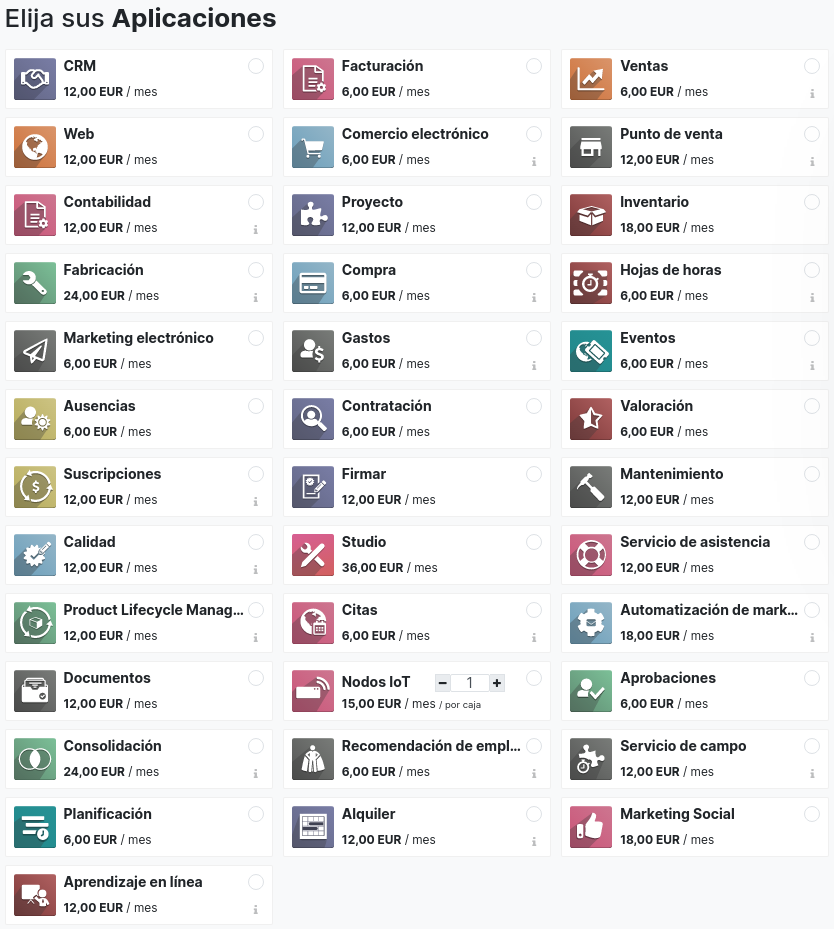
\includegraphics[scale=0.4]{archivos/odooModules.png}
\caption{Compra de módulos de Odoo}
\label{fig:odooModules_compra}
\end{figure}
\clearpage
\begin{figure}[h]
\centering
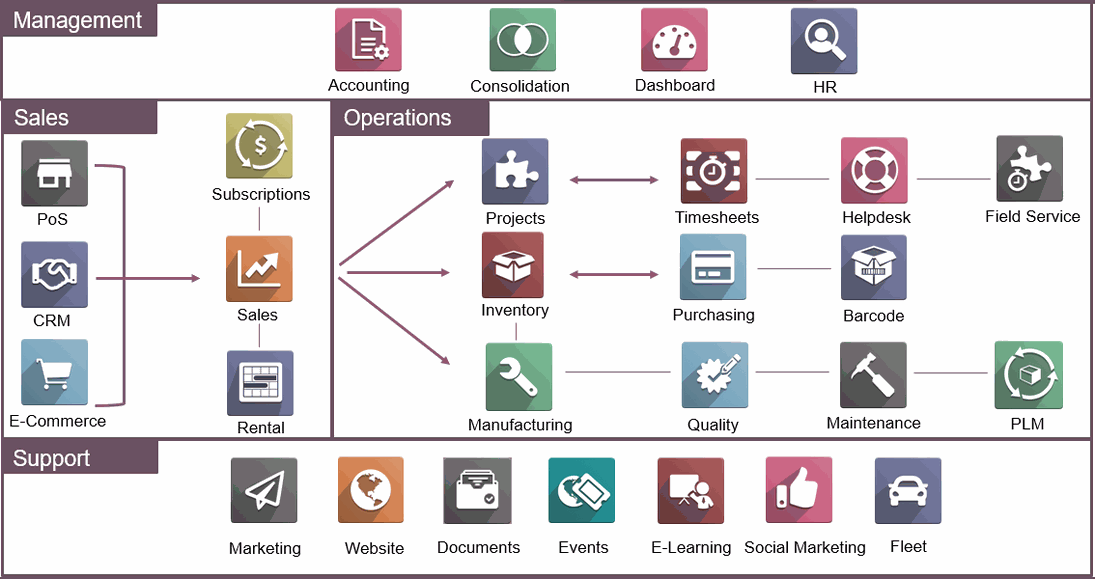
\includegraphics[scale=0.38]{archivos/odooModules2.png}
\caption{Comunicación entre módulos de Odoo}
\label{fig:odooModules_comunicacion}
\end{figure}
\par Podríamos listar las siguientes ventajas:
\begin{itemize}
    \item Bajo coste
    \item Open source
    \item Capacidad de operar en la nube
    \item Inyección de módulo hechos a mano
\end{itemize}
Y las siguientes desventajas:
\begin{itemize}
    \item Tiene coste
    \item Necesita mantenimiento informático avanzado
    \item Curva de aprendizaje y estudio de módulos para la adopción
\end{itemize}
%\vspace{0.5em}
\par A pesar de tener ventajas en la instalación y puesta en marcha frente a otras soluciones como \citep{oracleERP} o \citep{sapERP} y a pesar de ser open source con una comunidad amplia de desarrolladores y con miles de aplicaciones, sigue siendo demasiado complejo para lo que necesitamos. La propia plataforma recomienda contactar con un distribuidor para que ayude al negocio a implantar la solución dado que hacen falta conocimientos informáticos extensos. Recordamos que pretendemos una solución simple de usar y poner en marcha.
%\vspace{0.5em}
\par Por lo que terminamos por descartar las soluciones ERP que el mercado pone a nuestra disposición. Las necesidades del economato social son muy concretas y decidimos que hacer ad hoc una solución verdaderamente libre nos resuelve el problema que tenemos. Además, nos permite escalar y mantener la aplicación de forma libre si la solución saltase a otros economatos sociales.
% --------------------------------------------------------------
% --------------------------------------------------------------
% --------------------------------------------------------------
\clearpage
\subsection{Decidiendo arquitectura}
Dadas las premisas de arquitectura, para este proyecto optamos por estudiar las siguientes posibilidades:
\begin{itemize}
    \item Raspberry pi y Do It Yourself (DiY)
    \item Computación elástica bajo demanda
    \item Serverless
\end{itemize}
% --------------------------------------------------------------
% --------------------------------------------------------------
% --------------------------------------------------------------
\subsubsection{Raspberry pi (DIY)}
\begin{figure}[h]
\centering
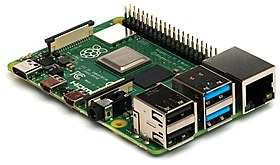
\includegraphics[scale=0.5]{archivos/RPi_4.jpg}
\caption{Raspberry Pi 4 Modelo B}
\label{fig:rpi4}
\end{figure}
\vspace{1em}
\par La Raspberry Pi fue nuestra primera idea, debido a su condición de software de código abierto, bajo coste de adquisición, reducido espacio y poco consumo.
%\vspace{1em}
\par La Raspberry Pi es una serie de ordenadores de placa reducida y bajo coste desarrollado en Reino Unido. Su objetivo principal ha sido siempre poner a disposición de todo el mundo el poder de la informática con un ordenador reducido en espacio y coste. Cuando se creó, se pretendía promocionar la enseñanza informática en las escuelas, pero terminó siendo mucho más popular de lo que se esperaba. Como se muestra en la figura \ref{fig:rpi4}, no trae ningún tipo de periférico ni carcasa. Sin embargo, hay packs de todo tipo que pretenden facilitar la adopción del hardware.
\begin{figure}[h]
\centering
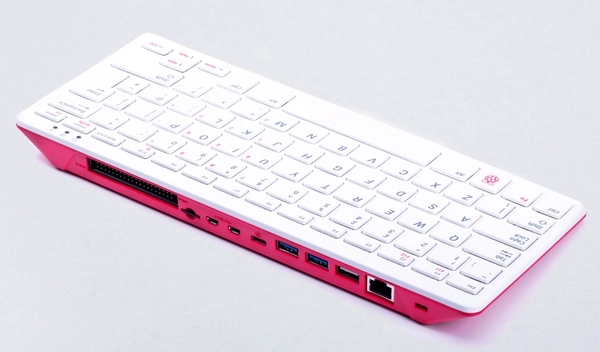
\includegraphics[scale=0.4]{archivos/rpi4keyboard.png}
\caption{Raspberry Pi integrada en el interior de un teclado}
\label{fig:rpi4keyboard}
\end{figure}
\begin{figure}[h]
\centering
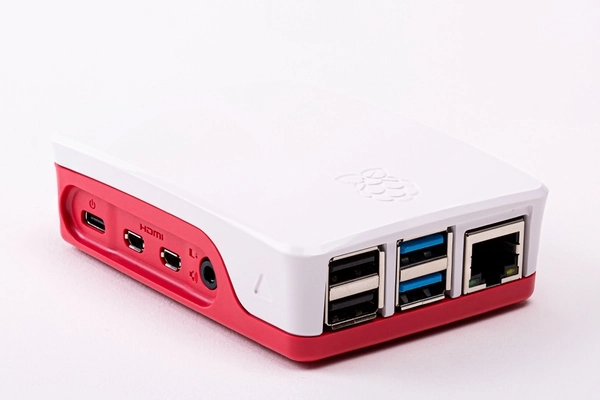
\includegraphics[scale=0.4]{archivos/rpi4case.png}
\caption{Raspberry Pi protegida con funda}
\label{fig:rpi4case}
\end{figure}
%\vspace{1em}
\par En cuanto a la distribución del hardware, la Raspberry Pi Foundation no indica expresamente que el hardware sea libre o con derechos de marca. Sin embargo, sí explican en su web oficial que cualquiera puede convertirse en revendedor o redistribuidor de las tarjetas Raspberry Pi, dando a entender que es un producto con propiedad registrada pero que permite el uso libre tanto a nivel educativo como particular.
%\vspace{1em}
\par Su software sí es código abierto. Su sistema operativo se basa en Debian y se hace llamar Raspberry Pi OS. El procesador es ARM, por lo que la paquetería debianita tiene que pasar un proceso de adaptación y recompilación para poder usarse en la Pi OS.
%\vspace{1em}
\par Todas estas características fueron las que nos incitó a considerarla como una buena solución a lo que se no estaba planteando. Pero el conocimiento de sistemas informáticos iba a ser una carga muy elevada en caso de avería, mantenimiento o escalabilidad. Además, una última situación nos hizo deshacernos de las Pis como solución hardware, la disponibilidad del software.
%\vspace{1em}
\par Una de nuestras premisas era tener la posibilidad de implantar el sistema en otros posibles economatos sociales, los cuales podrían encontrarse en diferentes localidades. Haber resuelto el host de la aplicación web en una raspberry pi, podría habernos planteado problemas de arquitectura y distribución en etapas futuras del proyecto.
%nos habría planteado problemas de arquitectura mucho más elevados más adelante.
%Una de nuestras premisas era tener en cuenta la capacidad de salto a otros economatos sociales, tanto de la zona, como de la ciudad; 
\begin{itemize}
    \item ¿Dónde deberá localizarse el servidor una vez haya más de una sede haciendo uso?
    \item ¿Deberíamos distribuir su ejecución para abordar situaciones en las que el nodo principal se quede sin luz?
    %por si el nodo principal se queda sin luz?
\end{itemize}
En seguida caímos en que si bien es una problemática resoluble, teníamos soluciones al alcance de la mano y por muy bajo coste: Los servicios de computación en la nube bajo demanda.
% --------------------------------------------------------------
% --------------------------------------------------------------
% --------------------------------------------------------------
\clearpage
\subsubsection{Computación elástica bajo demanda (Cloud)}
Dado que la arquitectura hardware mantenida por nosotros no iba a ser viable a la larga, pusimos la vista en la computación elástica.
%\vspace{1em}
\par Los servicios Cloud nacen para dar una recurso muy simple de explicar y no tan fácil de proveer, capacidad infinita de procesamiento. Un servicio cloud no es simplemente un software que corre en el ordenador de otro en lugar del propio, es la escalabilidad (casi) sin límites y bajo demanda, lo que le da potencia como idea. Hoy en día hay múltiples proveedores de servicios cloud, siendo AWS, Azure y Digital Ocean los más conocidos.
\begin{table}[h]
\centering

\includegraphics[scale=0.2]{archivos/aws.png}

\includegraphics[scale=0.2]{archivos/azure.png}

\includegraphics[scale=0.08]{archivos/digitalocean.png}
\caption{Logos de Aws, Azure y Digital Ocean}
\end{table}
%\vspace{1em}
\par Dada la experiencia laboral y personal como arquitecto \emph{cloud} en servicios AWS, valoramos con mayor criterio y peso el desarrollo de una solución basada en la nube. Esta opción presenta ventajas en coste y funciones que la hacen más apropiada para los objetivos del proyecto.
%Dado que yo tengo experiencia laboral y personal como arquitecto cloud en servicios aws y me estoy preparando el examen oficial, decidimos sin pensárnoslo mucho en estudiar nuestra solución como nativa cloud haciendo uso de los servicios Aws. 
Si bien Aws tiene capas gratuitas, éstas son temporales en caso de la computación y son circulares en caso de la transmisión de datos. Dado nuestro cliente y nuestro estudio de casos de uso, sabíamos que podríamos usar las capas gratuitas de transferencia de datos sin problema. Sin embargo, el hosting podría presentar alguna dificultad, pero valorando las ventajas por encima de los posibles problemas estimamos conveniente continuar en esta dirección.
%sí podría suponer una traba. A pesar de ello, proseguimos.
%\vspace{1em}
\par En concreto, con AWS, usaríamos una de las máquinas de computación elástica más pequeña de las que disponemos para montar nuestro servidor web, haciendo uso de imágenes dockerizadas y distribuídas por el propio registro de imágenes de Aws. En todo momento hemos querido mantener el estándar y el open source, esto facilitaría la recepción de voluntarios informáticos. Las máquinas que AWS provee (llamado \citep{ec2AWS}), es descrito como `Capacidad informática segura y de tamaño ajustable que admite prácticamente cualquier carga de trabajo`.
%\vspace{1em}
\par La parte buena de usar esta opción es la capacidad de usar sus servicios bajo demanda. Podemos hacer crecer y disminuir máquinas conforme necesitemos, balancear la carga entre varios nodos e incluso aumentar nuestro porcentaje de disponibilidad usando la Route 53. Esta última función mencionada, nos permite que en caso de que una región dejara de estar disponible, automáticamente el trafico sea redirigido a la región más cercana. Además, para evitar configuraciones y mantenimiento, habríamos usado una base de datos \emph{adhoc} RDS. Teniéndolo todo centralizado en una misma red podemos minimizar la espera por latencia y proteger el acceso y DDOS de nuestra máquina usando el servicio de ApiGateway. El \emph{frontend} puede ser desatendido y almacenado en un S3, con lo que podríamos obtener un sistema distribuido y cacheado por el servicio de CloudFront.
%El frontend puede ser desatendido, almacenado en un S3 de bajo coste, distribuido y cacheado por el servicio de CloudFront.
\begin{figure}[h]
\centering
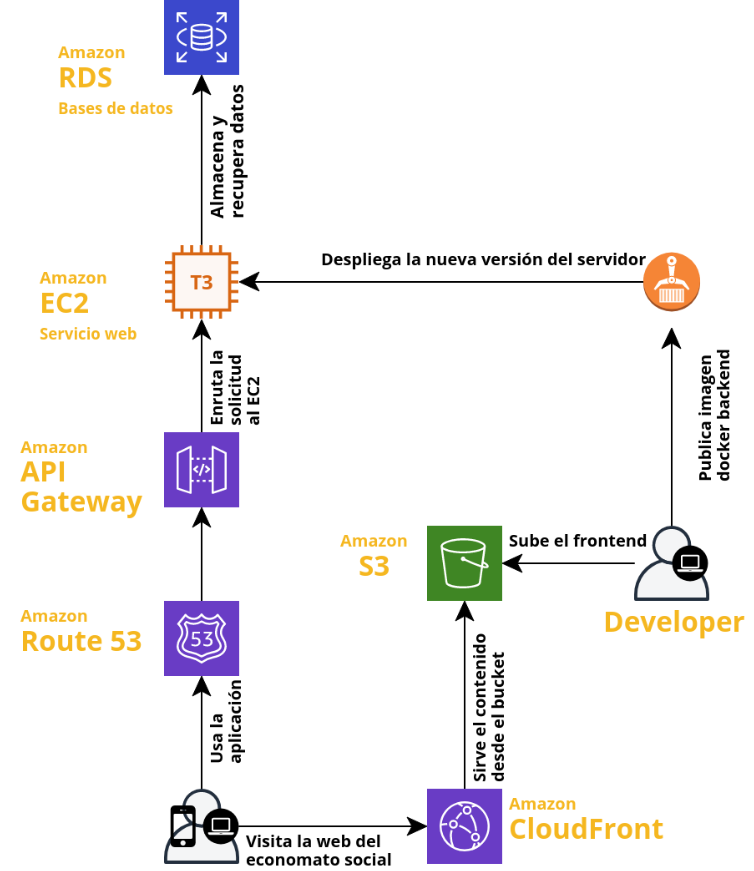
\includegraphics[scale=0.5]{archivos/arquitecturaAws.png}
\caption{Arquitectura simplificada}
\end{figure}
\clearpage
\begin{figure}[h]
\centering
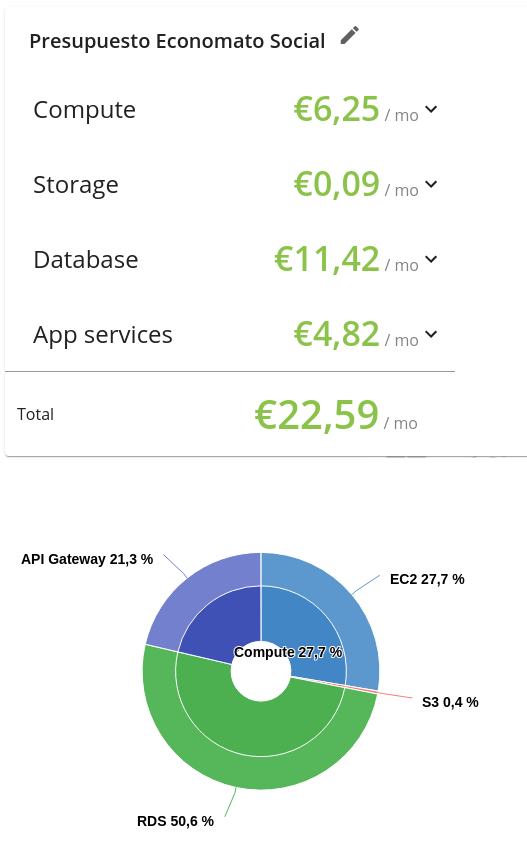
\includegraphics[scale=0.6]{archivos/budgetAws.png}
\caption{Presupuesto simplificado}
\end{figure}
\clearpage
%\vspace{1em}
\par Los puntos que hemos evaluado hacen de la arquitectura un proyecto ideal, ya que presenta una estructura sencilla de manejar para alguien con formación en la materia. Sin embargo, 
%Todo esto hace de la arquitectura un proyecto ideal, una estructura sencilla de manejar para alguien con conocimientos, pero aunque hubiésemos podido aceptar el presupuesto, 
nos volvimos a topar con la misma problemática que en el caso de la Raspberry Pi. ¿Qué ocurriría si una máquina deja de estar accesible? ¿Y si hay un problema en la configuración de red o de acceso por grupos de seguridad? ¿Y si alguien toca sin querer algo que no debe en un despliegue? Nuestro objetivo de no ceder el mantenimiento a la posibilidad de tener siempre conocimientos informáticos disponibles en el voluntariado, era más fuerte que intentar idear una arquitectura digna de proyectos modernos.
%\vspace{1em}
\par Sólo nos quedaba una carta que jugar, una forma de explotar el cloud que ya había usado en proyectos anteriores, y que podría ser lo que nos permitiese centrar el conocimiento informático voluntario en el desarrollo y mantenimiento de la aplicación; permitiéndonos ignorar la disponibilidad del servicio y configuración de las máquinas: el Serverless.
% --------------------------------------------------------------
% --------------------------------------------------------------
% --------------------------------------------------------------
\clearpage
\subsubsection{Serverless (Cloud)}
Como ya hemos ido hablando, el sector privado tiende cada vez más hacia los servicios en la nube, sobretodo el sector comercial, debido a la capacidad de contratar y configurar soluciones a medida de las necesidades de cada uno. Dentro de la oferta de servicios cloud existe el uno llamado Serverless Computing, una de las prácticas más recientes, y comúnmente conocido como FaaS (Function as a Service).
%\vspace{1em}
\par El primer concepto que nos atrajo para adoptar esta solución es la propia descripción del Serverless Computing o Arquitectura Serverless. Éste viene a ser un modelo que permite a los usuarios crear y ejecutar aplicaciones o procesos sin entrar en contacto con el servidor subyacente. Esta funcionalidad es justo lo que queremos, un entorno en la nube en el que es el propio proveedor el que se ocupa del suministro, gestión y escalado del servicio. Esto además tiene un punto fuerte para nuestra intención de adopción futura, podemos centrar toda nuestra atención y esfuerzo en el desarrollo y en la ejecución del software, ahorrando tareas y conocimientos al equipo implicado.
%\vspace{1em}
\par Normalmente, los proveedores de Serverless no sólo son responsables de que los recursos del servidor estén siempre disponibles, si no también lo son de garantizar la disponibilidad del servicio, es decir, seguridad anticaída. Normalmente este tipo de servicios tienen un modelo de pago por uso, el cual abordaremos después.
\subsubsection{¿Cómo funciona?}
En una infraestructura serverless, la gestión del hardware por parte del proveedor es esencial. El único desafío con el que tienen que lidiar los usuarios es integrar su software o su lógica, incluidas las funciones adecuadas, en el espacio alquilado en la nube. El acceso a estas funciones se puede realizar de dos maneras:
\begin{itemize}
    \item de forma asíncrona, a través de eventos
    \item de forma síncrona, según el modelo Cliente-Servidor clásico
\end{itemize}
%\vspace{1em}
\par La forma de uso asíncrona ofrece la ventaja de evitar acoplamiento entre las funciones y mantener la demanda de recursos en un nivel bajo durante la ejecución. Un ejemplo de función asíncrona sería que al cargar una imagen se cree también un icono en miniatura. Son funciones atómicas, que aportan mucho control en el código, mayor simplicidad y reducción de gastos, dado que sólo se paga cuando se usa. Además, los problemas de optimización también son más fáciles de acotar, y se puede decidir añadir recursos, en vez de optimizar una función que tenga un rendimiento deficiente.% pero no necesariamente a todo el sistema.
%los problemas de optimización también son más fáciles de acotar, y se puede decidir  recursos a optimizar una función que funcione deficientemente pero no necesariamente a todo el sistema.
%\vspace{1em}
\par El uso que nosotros vamos a darle al Serverless es la función síncrona, vamos a usar el servicio para poder mantener levantado un servidor web sin tener que estar pendientes de mantener el sistema, actualizarlo o configurarlo. En concreto, vamos a usar la solución que provee Heroku, un proveedor de servicios Serverless con una generosa capa gratuita que a éste trabajo le vendrá de perlas. La única limitación que pueda importarnos, de las que tiene Heroku en su capa gratuita, es que los servicios mueren tras 5 minutos sin uso, haciendo que la siguiente petición tarde un poco más. Esto encaja a la perfección con nuestras necesidades pues, a priori, se le va a dar uso al sistema un par de días a la semana.
%\vspace{1em}
\par A diferencia de una infrastructura de plataforma como servicio, el proveedor Serverless no facilita para ello un entorno de trabajo duradero para todo el tiempo de trabajo, si no que aporta de manera puntual y en tiempo real aquellos recursos que se requieren durante el tiempo de ejecución de la llamada a la función. A pesar de llamarse Serverless, obviamente se ejecuta en servidores detrás del telón, aunque el usuario nunca lo perciba.
\subsubsection{Vista general de ventajas y desventajas}
Las infraestructuras convencionales en la nube permiten al usuario administrar y eliminar el hardware que se requiere, pero a menudo, esto requiere grandes esfuerzos a nivel de administración y micro-gestión. Lo que pretende el Serverless es minimizar esto al máximo.
%\vspace{1em}
\par Podríamos considerar las siguientes ventajas y desventajas
\begin{itemize}
    \item Ventajas
    \begin{itemize}
        \item Escalamiento y administración de los recursos necesarios por parte del proveedor
        \item Suministro ágil de los recursos en tiempo real, en función del consumo en cada momento
        \item Cobro únicamente por uso al milisegundo
        \item Gran tolerancia a errores gracias a la infraestructura flexible de hardaware
    \end{itemize}
    \item Desventajas
    \begin{itemize}
        \item Acceso restringido a los sistemas e incapacidad de configuración de éstos
        \item Grandes proyectos basados en funciones asíncronas pueden suponer un gran esfuerzo de implementación
        \item Gran dependencia del proveedor, posibles dificultades de migración
        \item Procesos de monitorización y depuración de errores más complejos
    \end{itemize}
\end{itemize}
\subsubsection{Cuándo se usa el principio \emph{Serverless}}
El serverless computing ha sido concebido principalmente para el intercambio efímero de datos de aplicaciones web y de negocios en la nube, aunque acabó abarcando servicios más complejos y con una vida de ejecución más larga pero basándose en las mismas premisas: escalabilidad elástica en tiempo real adecuándose al uso, sin que el usuario tenga que hacerse cargo de configuraciones de sistemas y redes.
%\vspace{1em}
\par Los escenarios más comunes del \emph{Serverless} son los siguientes:
\begin{itemize}
    \item Proxy API: muchas aplicaciones comerciales antiguas cuenta con interfaces complejas y lentas. Mediante el serverless se puede crear una capa de abstracción alternativa para poder acceder a estas aplicaciones mediante una API REST mucho más simple
    \item Serverless Backend: el \emph{serverless computing} también se usa cada vez más para construir y soportar todo el \emph{backend} de una aplicación en la nube. \emph{Backend as a Service}.
    \item Procesamiento de datos no estructurados: hoy en día, es imposible imaginar un entorno de negocios sin \emph{big data}. En este contexto, el \emph{serverless} se muestra como un gran aliado para procesar este tipo de información.
    \item Ejecución de tareas según horario: una gran cantidad de demanda de este tipo de funciones en un horario definido, un disparador que ejecuta alguna automatización aislada como backups de bases de datos, reorganización de datos, etc.
    \item Aplicación de asistentes y chat bots: Normalmente este tipo de aplicaciones son sin estado y se conectan con servicios de modelos inteligentes más complejos. Estas interfaces en \emph{serverless} están en auge.
\end{itemize}
% --------------------------------------------------------------
% --------------------------------------------------------------
% --------------------------------------------------------------
\subsubsection{Ejemplos de uso con heroku}
\begin{figure}[h]
\centering
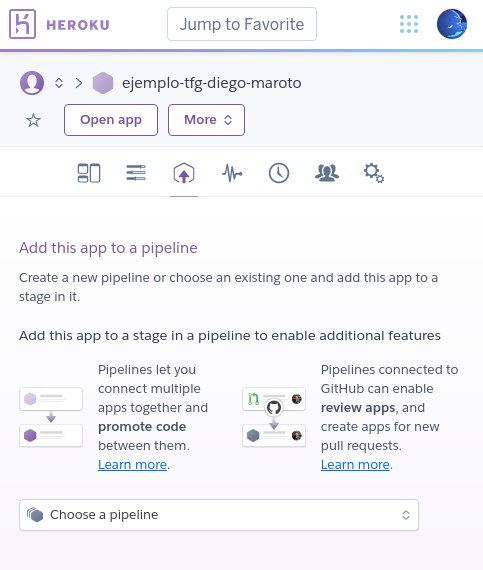
\includegraphics[scale=0.5]{archivos/heroku01.png}
\caption{Configurando proyecto en Heroku}
\end{figure}

\begin{figure}[h]
\centering

\includegraphics[scale=0.5]{archivos/heroku02.png}
\caption{CI/CD en Heroku}
\end{figure}

\begin{figure}[h]
\centering
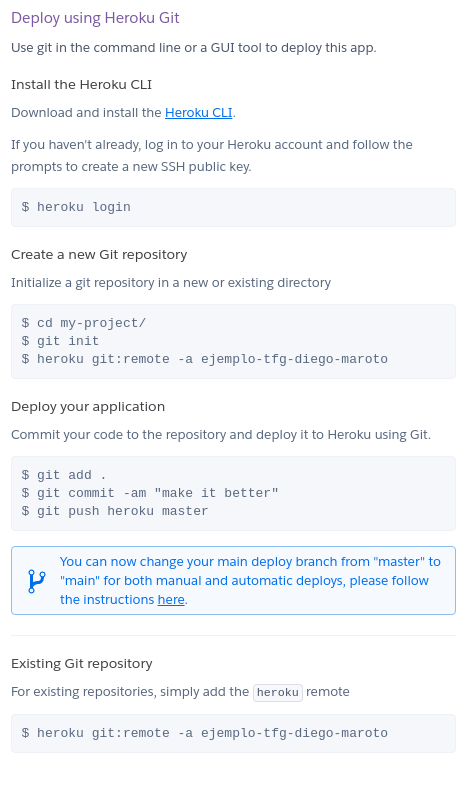
\includegraphics[scale=0.5]{archivos/heroku03.png}
\caption{Ejemplo de uso de Heroku por línea de comandos}
\end{figure}
\clearpage
% --------------------------------------------------------------
% --------------------------------------------------------------
% --------------------------------------------------------------
\clearpage
\subsection{Stack FrontEnd/BackEend}
Una de nuestras principales preocupaciones, como se ha mencionado en apartados anteriores, es la escalabilidad del proyecto en cuanto a la facilidad de colaboración técnica por parte de los voluntarios. A partir de esta premisa, estuvimos estudiando qué lenguajes de programación podrían encajar en esta dinámica.
%\vspace{1em}
\par En el mundo del desarrollo, la plataforma más usada es Stack Overflow; en esencia es un foro tecnológico donde usuarios escriben sus dudas y otros usuarios intentan resolverlas. Stack Overflow hace una encuesta todos los años para extraer datos demográficos, económicos y tecnológicos sobre la comunidad tecnológica mundial. Decidimos basarnos en la encuesta de 2020 \citep{techSurveyStackOverflow} para valorar el \emph{stack} a usar.
%\vspace{1em}
\par Como se aprecia en la encuesta, javascript es el más usado tanto profesional como amateur. Además, encaja en nuestra idea inicial, en la que consideramos usar el mismo lenguaje para \emph{frontend} y \emph{backend}. Dado que va a ser un proyecto dilatado en el tiempo, un lenguaje de tipado estático sería una buena forma de agilizar la curva de aprendizaje del proyecto y recortar la barrera de entrada a los posibles desarrolladores voluntarios; así pues, dado que Typescript está en el top 10 y podemos considerarlo javascript, optamos por usarlo.
%\vspace{1em}
\par Una vez decidido el lenguaje, queda la decisión de si usar frameworks o no. No usarlos puede ser potente en un inicio, pues permite la flexibilidad de montar el sistema como se quiera y definir unas pautas. Estas pautas preferiríamos que pudiesen ponerse en tela de juicio lo menos posible, así que optaremos por \emph{frameworks}. De esta manera, la forma de hacer las cosas será siempre la misma independientemente de quién trabaje en el proyecto.
%\vspace{1em}
\par En javascript es muy común el stack MEAN (Mongo, Express, Angular y Nodejs), y para facilitar el desarrollo de backend y frontend, usaremos para el backend Nodejs con Express y el framework Nestjs; un framework disponible en typescript cuya estructura MVC es muy parecida a Angular, de esta forma, un desarrollador frontend podrá pivotar al backend y viceversa con muy poco problema.
%\vspace{1em}
\par Para la persistencia de datos se había propuesto MongoDB desde un inicio, y éste encaja con Javascript a la perfección. Los documentos de ambos se anotan en JSON, lo que permite una integración intuitiva y sencilla. Además, MongoDB tiene capa gratuita en su servicio cloud Compass y es justo lo que queremos. 
%\vspace{1em}
\par Teniendo en cuenta los puntos mencionados a lo largo de este apartado, quedan definidas las herramientas que se utilizarán.
%Y de esta forma queda decidido, se usará 
Typescript con Nestjs para el backend, Typescript con Angular para el frontend y MongoDB para la persistencia de datos. 
\clearpage
	% Plantilla: Se muestran listas
%%%%%%%%%%%%%%%%%%%%%%%%%%%%%%%%%%%%%%%%%%%%%%%%%%%%%%%%%%%%%%%%%%%%%%%%
% Plantilla TFG/TFM
% Escuela Politécnica Superior de la Universidad de Alicante
% Realizado por: Jose Manuel Requena Plens
% Contacto: info@jmrplens.com / Telegram:@jmrplens
%%%%%%%%%%%%%%%%%%%%%%%%%%%%%%%%%%%%%%%%%%%%%%%%%%%%%%%%%%%%%%%%%%%%%%%%

\chapter{Objetivos (Con ejemplos de tablas)}
\label{objetivos}

\section{Tablas}
Ahora veremos otra estructura más: las tablas.


Aquí va una tabla\footnote{En http://www.tablesgenerator.com/ se puede encontrar un generador On-Line de tablas para \LaTeX} para que se vea cómo insertar una tabla simple dentro del documento.

\begin{lstlisting}[style=Latex-color]
\begin{table}[h]
	\centering
	\begin{tabular}{lllll}
		&columna A&columna B&columna C\\
		\hline
		fila 1&fila 1, columna A & fila 1, columna B & fila 1, columna C\\
		fila 2&fila 2, columna A & fila 2, columna B & fila 2, columna C\\
		fila 3&fila 3, columna A & fila 3, columna B & fila 3, columna C\\ \hline
	\end{tabular}
	\caption{Ejemplo de tabla.}
	\label{tabladeejemplo}
\end{table}
\end{lstlisting}

\begin{table}[h]
	\centering
	\begin{tabular}{lllll}
		&columna A&columna B&columna C\\
		\hline
		fila 1&fila 1, columna A & fila 1, columna B & fila 1, columna C\\
		fila 2&fila 2, columna A & fila 2, columna B & fila 2, columna C\\
		fila 3&fila 3, columna A & fila 3, columna B & fila 3, columna C\\ \hline
	\end{tabular}
	\caption{Ejemplo de tabla.}
	\label{tabladeejemplo}
\end{table}

\LaTeX~usa un sistema de parámetros para ``decorar'' las tablas. Puedes consultar estos parámetros en la tabla \ref{tabla_parametros} de la página \pageref{tabla_parametros}. La tabla se ubicará donde, a juicio de \LaTeX, menos moleste por lo que puede no aparecer necesariamente donde se ha insertado en el texto original. 

Existe la posibilidad de forzar que las tablas, figuras u otros objetos aparezcan en la zona del texto que se desea aunque en ocasiones puede dejar grandes espacios en blanco. El comando a utilizar es:
\begin{lstlisting}[style=Latex-color]
\FloatBarrier	
\end{lstlisting}
Que introducido justo después de una tabla, figura, etc (despues del comando \textbackslash end\{...\}) fuerza la aparición en el texto, empujando el contenido.

\begin{table}[ht]
\centering
\begin{tabular}{|c|L{0.8\textwidth}|}
\hline
Parámetro & \multicolumn{1}{c|}{Significado} \\ \hline
\texttt{h} & Situa el elemento flotante \emph{preferentemente}
(es decir, si es posible) en la situación exacta donde se incluye este \\
\texttt{t} & Sitúa el elemento en la parte de arriba de la página \\
\texttt{b} & Sitúa el elemento en la parte de abajo de la página \\
\texttt{p} & Sitúa el elemento en una página aparte dedicada sólo a
elementos flotantes; en el caso del formato \texttt{article},
ésta se sitúa al final del documento, mientras que para al book es
colocada al final de cada capítulo \\ \hline
\end{tabular}
\caption{Parámetros optativos de los entornos flotantes}
\label{tabla_parametros}
\end{table}
\FloatBarrier

También es posible elegir el ancho de cada columna y la orientación del texto en cada una.
Por ejemplo:

\begin{lstlisting}[style=Latex-color]
\begin{table}[ht]
	\centering
	\begin{tabular}{|C{2cm}|C{2cm}|C{2cm}|C{2cm}|} % 4 columnas de 2cm - texto centrado y con bordes
		\hline
		\multicolumn{4}{|c|}{\textbf{\begin{tabular}[c]{@{}c@{}}FUENTE: TRÁFICO RODADO\\ HORARIO: TARDE\end{tabular}}} \\ \hline
		\textbf{dB(A)} & \textbf{Población expuesta tarde} & \textbf{\%} & \textbf{\scriptsize{CENTENAS}} \\ \hline
		\textbf{\textgreater70} & 0 & 0,000 & 0 \\ \hline
		\textbf{65 - 70} & 348,9 & 9,792 & 3 \\ \hline
		\textbf{60 - 65} & 1594,7 & 44,757 & 16 \\ \hline
		\textbf{55 - 60} & 322,1 & 9,040 & 3 \\ \hline
		\textbf{50 - 55} & 0 & 0,000 & 0 \\ \hline
		\textbf{\textgreater50} & 1297,3 & 36,410 & 13 \\ \hline
		\textbf{TOTAL} & 3563 & 100 & 35 \\ \hline
	\end{tabular}
	\label{my-label}
\end{table}	
\end{lstlisting}

\LaTeX~genera esto:
\begin{table}[ht]
	\centering
	\begin{tabular}{|C{2cm}|C{2cm}|C{2cm}|C{2cm}|}
		\hline
		\multicolumn{4}{|c|}{\textbf{\begin{tabular}[c]{@{}c@{}}FUENTE: TRÁFICO RODADO\\ HORARIO: TARDE\end{tabular}}} \\ \hline
		\textbf{dB(A)} & \textbf{Población expuesta tarde} & \textbf{\%} & \textbf{\scriptsize{CENTENAS}} \\ \hline
		\textbf{\textgreater70} & 0 & 0,000 & 0 \\ \hline
		\textbf{65 - 70} & 348,9 & 9,792 & 3 \\ \hline
		\textbf{60 - 65} & 1594,7 & 44,757 & 16 \\ \hline
		\textbf{55 - 60} & 322,1 & 9,040 & 3 \\ \hline
		\textbf{50 - 55} & 0 & 0,000 & 0 \\ \hline
		\textbf{\textgreater50} & 1297,3 & 36,410 & 13 \\ \hline
		\textbf{TOTAL} & 3563 & 100 & 35 \\ \hline
	\end{tabular}
	\label{my-label}
\end{table}	

Donde C\{2cm\} indica que la columna tiene el texto centrado y un ancho de 2 cm. Tambien se puede utilizar L\{\} o R\{\} para poner el texto a la izquierda o derecha y definir un ancho concreto.

Páginas como \url{https://www.tablesgenerator.com/} ayudan a realizar tablas fácilmente, es lo más recomendado, ahorra mucho tiempo de trabajo y luego si falta algún detalle se puede retocar en el documento.

El formato estándar de las columnas es c, l o r, así lo genera la web mencionada antes, pero una vez generada puedes cambiar ese formato por el definido anteriormente para ajustar el ancho de las columnas, o mantenerlo así si el resultado ya es el deseado.

\par Para conocer más sobre las tablas puedes leer manuales como este: \url{https://latexlive.files.wordpress.com/2009/04/tablas.pdf} que contiene muchos ejemplos y explicaciones.


\section{Otros diseños de tablas}

% EJEMPLO 1
\begin{table}[ht]
	\centering
	{\scalefont{0.9}
	\begin{tabular}{@{}lcc@{}}
	\toprule
	Modelo			& 	15LEX1600Nd	&	15P1000Fe V2	 	\\ \midrule
	fs ($Hz$)		& 	41          & 	45           	\\
	Re ($ohm$)		& 5.5         	& 5.2         	 	\\
	Le ($\mu H$)	& 1600        	& 1500         		\\
	Bl ($N/A$)		& 25.7        	& 27.4         		\\
	M\textsubscript{MS} ($g$)		& 175	& 157		\\
	C\textsubscript{MS} ($\mu m/N$)	& 84		& 78			\\
	R\textsubscript{MS} ($kg/s$)		& 6.8 	& 7.6   	 	\\
	d ($cm$)		& 33.5			& 33           		\\
	Vas ($dm^3$)   	& 91          	& 80.7         		\\
	$Q_\text{TS}$  	& 0.36        	& 0.30         		\\
	$Q_\text{MS}$  	& 6.6         	& 5.9          		\\
	$Q_\text{ES}$  	& 0.38        	& 0.31         		\\
	Sens (dB @ 2.83V/1m) & 96      	& 98           		\\
	$\eta$          & 1.7\%       	& 2.4\%        		\\
	Sd ($cm^2$)   	& 880         	& 855          		\\ \bottomrule
	\end{tabular}
	}
	\caption{Parámetros de los altavoces elegidos de la marca Beyma\textsuperscript{\tiny\textregistered}.}
	\label{tablaparametros}
\end{table}

% EJEMPLO 2
\begin{table}[ht]
\centering
\begin{tabular}{l|l|c|c|c|c||c|c|c|c} %l:left c:center r:right |:table lines
\cmidrule[1pt]{3-10}                  % 1pt is the thickness 3-10 is column number
\multicolumn{2}{c|}{}&\multicolumn{4}{c||}{140PU}&\multicolumn{4}{c}{50PU} \\\cmidrule{3-10}
\multicolumn{2}{c|}{}&\multicolumn{2}{c|}{Phase II}&\multicolumn{2}{c||}{Phase I}&\multicolumn{2}{c|}{Phase II}&\multicolumn{2}{c}{Phase I}\\\midrule
\multicolumn{2}{c|}{\# BJet}&$ \geq 4 $ & 2 or 3 &$ \geq 4 $ & 2 or 3&$ \geq 4 $ & 2 or 3 &$ \geq 4 $ & 2 or 3 \\\midrule
\multicolumn{2}{c|}{\# Bkg} & 123 & 76 & 12 & 7 & 84 & 35 & 7 & 3 \\\midrule\midrule
\multirow{4}{3mm}{\begin{sideways}\parbox{15mm}{Asimov}\end{sideways}}
& NM1 & 13 & 6 & 9 & 3 & 15 & 9 & 11 & 4 \\
& NM2 & 6 & 2 & 4 & 1 & 7 & 3 & 5 & 1 \\
& NM3 & 3 & 1 & 2 & 0 & 4 & 1 & 2 & 0 \\
& STC & 6 & 3 & 4 & 1 & 7 & 5 & 5 & 2 \\\midrule
\end{tabular}
\caption{Ejemplo 2}
\end{table}








		% Plantilla: Se muestran tablas
%%%%%%%%%%%%%%%%%%%%%%%%%%%%%%%%%%%%%%%%%%%%%%%%%%%%%%%%%%%%%%%%%%%%%%%%
% Plantilla TFG/TFM
% Escuela Politécnica Superior de la Universidad de Alicante
% Realizado por: Jose Manuel Requena Plens
% Contacto: info@jmrplens.com / Telegram:@jmrplens
%%%%%%%%%%%%%%%%%%%%%%%%%%%%%%%%%%%%%%%%%%%%%%%%%%%%%%%%%%%%%%%%%%%%%%%%

\chapter{Metodología}
\label{metodologia}
En este apartado se van a describir las herramientas necesarias para el correcto desarrollo del proyecto. Éstas herramientas están comprendidas en lo que se puede llamar ingeniería del software, disciplina que comprende análisis del problema, estudio de la solución, el diseño del proyecto, el desarrollo del software, las pruebas que faciliten la integración continua y la adopción del sistema. Éste proyecto se ha llevado a cabo mediante etapas como las detallas a continuación:
\section{Requisitos mínimos}
Los requisitos mínimos que se deben cumplir para poder desarrollar el proyecto, probarlo y ponerlo en marcha son los siguientes:
\begin{itemize}
    \item Pc, smartphone o tablet de cualquier sistema operativo que posea un navegador moderno
    \item Si Pc, lector de código de barras independiente por usb o webcam
    \item Si smartphone o tablet, cámara integrada para poder leer códigos de barras
    \item Conexión estable a internet
\end{itemize}
\section{Fases del desarrollo}
Aquí se van a nombrar y explicar de forma introductoria las fases de desarrollo que se han seguido para llevar a cabo el proyecto:
\begin{itemize}
    \item Análisis de requisitos: es la primera etapa en la que se identificarán los conceptos importantes sobre el proyecto, tales como las necesidades del proyecto, las funcionalidades requeridas y los requisitos para su buen funcionamiento
    \item Diseño del proyecto: en esta etapa se redactan los casos de uso y se realizan los mockups para una primera impresión visual de la aplicación
    \item Desarrollo del software: en esta etapa se realiza la aplicación usando las etapas anteriores como guía
    \item Pruebas: en esta etapa, que va muy ligada al desarrollo del software, se preparan pruebas automatizadas que permitan cerciorarse de que las funcionalidades desarrolladas efectivamente funcionan, y lo siguen haciendo tras refactorizaciones o nuevos desarrollos en la aplicación.
\end{itemize}
\section{Metodología ágil utilizada}
En este proyecto se ha seguido la metodología ágil denominada SCRUM. Ésta se define como un proceso de gestión que reduce la complejidad en el desarrollo de productos para satisfacer las necesidades de los clientes.
\vspace{1em}
\par En este proyecto en particular, se ha desarrollado el software mediante sprints, sprints review y milestones, que se detallan a continuación:
\vspace{1em}
\par Sprint: Etapa de 3 semanas en las que se desarrollan los objetivos establecidos para el mismo
\vspace{1em}
\par Sprint review: Reunión en la que se realiza una revisión de lo desarrollado, bloqueos, problemas y soluciones, además de una retrospectiva y planificación del siguiente.
\vspace{1em}
\par Milestone: Conjunto de objetivos de desarrollo que marcan metas en el progreso. Se han usado junto a fechas, para poder estimar y considerar el alcance en función del tiempo disponible.

Gracias a la utilización de metodologías ágiles es posible obtener grandes beneficios como indica la empresa \citep{braventAgile} en un artículo:
\begin{itemize}
    \item Satisfacción del cliente a través de la entrega temprana y continua del software de valor.
    \item Proximidad del cliente y constante iteración con él, es parte del equipo y está presente en la toma de decisiones.
    \item Gestión regular de las expectativas del cliente y basada en resultados tangibles.
    \item Resultados anticipados (time to market).
    \item Flexibilidad y adaptación respecto a las necesidades del cliente, cambios en el mercado, etc.
    \item Gestión sistemática del Retorno de la Inversión (ROI).
    \item Capacidad para abordar los requisitos cambiantes, incluso si llegan tarde en el proceso de desarrollo.
    \item Equipo implicado y motivado ya que pueden usar su creatividad para resolver problemas y pueden decidir organizar su trabajo.
    \item Auto-superación: de forma periódica se evalúa el producto que se está desarrollando
    \item Priorizar los requerimientos de acuerdo a su valor.
    \item Se proporciona la mínima funcionalidad, de forma que solo se desarrolla lo necesario. Evita
escribir código innecesario.
    \item Calidad del producto obtenido. El software que funciona es la principal medida del
progreso.
    \item Pruebas continuas durante todo el desarrollo.
    \item Mejora la productividad y el control del tiempo requerido para realizar el proyecto.
    \item Permite dividir el trabajo en módulos minimizando los fallos y el coste.
    \item Si surge cualquier error, se sabe rápido, disminuyendo riesgos.
    \item Permite solucionar rápidamente los problemas que impiden que los equipos progresen.
\end{itemize}
\section{Herramientas hardware}
Este apartado trata de los dispositivos de hardware necesarios para el buen desarrollo del proyecto, a excepción del ordenador utilizado para realizar el proyecto, del cual se asume que es obligatorio pero no exclusivo.
\vspace{1em}
\par Dado que una de las necesidades del proyecto es leer códigos de barras, podemos hacerlo de dos formas en función de qué dispositivos tengamos a mano:
\begin{itemize}
    \item Lector manual de código de barras por usb, al usar Pc
    \begin{itemize}
        \item Es la forma más cómoda de leer un código de barras cuando alguien trae una donación al banco de alimentos. Es la forma más fiable, teniendo el dispositivo a mano, sin importar el tamaño del producto, el tamaño del código de barras ni si es transparente o con poco contraste de colores.
    \end{itemize}
    \item Webcam al usar Pc
    \begin{itemize}
        \item Es un poco más tedioso que el anterior, se debe coger el producto y sostenerlo delante de la webcam, que en función de la calidad de ésta no enfoque bien automáticamente. Sin contar que la calidad y contrastes de la impresión del código de barras es un factor que puede hacerlo ilegible frente a una cámara.
    \end{itemize}
    \item Cámara trasera del dispositivo móvil
    \begin{itemize}
        \item Es un poco más tedioso que el hardware adhoc, normalmente los voluntarios no estarán usando el móvil, deben hacer login expresamente para esto e ir a la edición del producto para añadir el EAN. Sin contar, como en la anterior, que la calidad y contrastes de la impresión del código de barras es un factor que puede hacerlo ilegible frente a una cámara.
    \end{itemize}
\end{itemize}
\section{Herramientas software}
En este apartado se va a realizar una descripción del propósito de cada una de las herramientas de software utilizadas y que han sido necesarias para la realización del proyecto.
\subsection{Documentación}
En este apartado se define el software necesario para crear la documentación y memoria, y distribuirla.
\begin{itemize}
    \item Dropbox: Gestor de archivos en la nube, permite documentos simples y colaborativos. Los primeros bocetos de las ideas a desarrollar fueron en esta plataforma.
    \item Overleaf: Gestor de documentos \LaTeX~ en la nube. La memoria se ha creado completamente en \LaTeX~ y online
    \item Github: Control de versiones en la nube, las versiones de la memoria se han ido publicando en el repositorio que contiene el proyecto.
\end{itemize}
\subsection{Planificación y cumplimiento de las etapas}
En este apartado se va a definir el software necesario para poder realizar una planificación temporal del proyecto, definiendo etapas y marcas temporales y una estructuración de tareas.
\begin{itemize}
    \item Github: Panel de proyecto. Github contiene un panel en los repositorios que permite crear y manejar proyectos, al estilo de un tablero canvan. Las tareas se pueden mover de forma automática siendo disparadas por commits o pull requests.
    \item Github: Issues. Github permite listar y crear tareas, dándole etiquetas y relacionándolas con proyectos y milestones para acomodar su gestión.
    \item Github: Milestones. Github permite crear milestones con fecha de inicio y fin. Las milestones pueden estar relacionadas con proyectos y contener tantas issues como se crea conveniente en la planificación. 
\end{itemize}
\subsection{Desarrollo}
En este apartado se va a comentar el software que se ha utilizado para la realización del backend y el frontend dentro del proyecto.
\begin{itemize}
    \item Git: Control de versiones que permite conectar con gestores remotos, en este caso Github.
    \item Heroku-cli: Control de Continuous Delivery integrado con Git, permite la entrega continua y el despliegue automático completamente integrado con el uso de las ramas del proyecto.
    \item Docker: Se ha usado docker para virtualizar MongoDB en local y así desarrollar y lanzar las pruebas automáticas contra la máquina local y no afectar a los datos de producción en compass.
    \item Jest: Librería de testing para javascript que facilita muchísimo el uso de mocks, stubs y espiarlos.
    \item Yarn: Gestor de paquetería para javascript, facilita el manejo de dependencias del proyecto.
    \item WebStorm: IDE de JetBrains, contiene todo lo necesario para desarrollar javascript, nodejs y typescript. Trae integración con git para facilitar el uso del control de versiones, comparación de ramas, secciones de código, code blame y resolución de conflictos; además integra gestión de baterías de testing con Jest.
\end{itemize}	% Plantilla: Se muestran figuras
%%%%%%%%%%%%%%%%%%%%%%%%%%%%%%%%%%%%%%%%%%%%%%%%%%%%%%%%%%%%%%%%%%%%%%%%
% Plantilla TFG/TFM
% Escuela Politécnica Superior de la Universidad de Alicante
% Realizado por: Jose Manuel Requena Plens
% Contacto: info@jmrplens.com / Telegram:@jmrplens
%%%%%%%%%%%%%%%%%%%%%%%%%%%%%%%%%%%%%%%%%%%%%%%%%%%%%%%%%%%%%%%%%%%%%%%%

\chapter{Desarrollo}
\label{desarrollo}
Este apartado va a ser el que contenga los detalles sobre la implementación de la aplicación, tanto frontend como backend, mostrando código, capturas de la misma y acceso a dos vídeos de las funcionalidades de una forma resumida.
\section{Funciones}
Una de las primeras cosas que se hizo antes de empezar el desarrollo, fue una tormenta de ideas para decidir las funcionalidades y el alcance de éstas en el proyecto; estableciendo de esta manera un producto mínimo viable que entregar.
\vspace{1em}
\par Las funcionalidades que se decidió entregar como mínimo fuero:
\begin{itemize}
    \item Gestión de usuarios: Capacidad de crear usuarios, activarlos y desactivarlos, cambiarles la contraseña y atomizar los roles y permisos.
    \item Gestión de almacenes: Capacidad de crear y editar almacenes, los almacenes son la entidad más alta de la aplicación, sólo comparten súper administradores entre sí.
    \item Leer EAN por hardware: Capacidad de leer los códigos de barras de los productos mediante un lector específico o la webcam.
    \item Recepción de pedidos: Capacidad de recibir pedidos de productos con limitaciones muy concretas configuradas en la creación del producto, limitar al máximo la capacidad humana de fallar en estas limitaciones.
    \item Recepción del pedido restricciones familiares: Las familias tienen restricciones de cuánto y cuántas veces pueden consumir productos del banco de alimentos. Capacidad automática de gestionar estas limitaciones, con la mínima interacción humana.
    \item Gestión de productos: Capacidad para añadir y editar productos. Éstos productos deben poder tener un EAN asociado y solicitar información pública de OpenFoodFacts para añadir información nutricional a su ficha. Hay bancos de alimentos que cuentan con personal sanitario al que puede resultarle útil tener esta información a mano.
    \item Facturación y caja: Capacidad de cobrar facturas y buscarlas por rango de fechas para consultas posteriores.
    \item Impresión de facturas: Capacidad de ver las facturas maquetadas para imprimirlas fácilmente.
    \item Expedición de pedidos: Capacidad de ver qué pedidos están pendientes de despachar para que almacén pueda prepararlos con antelación.
    \item Dashboard con gráficas: Capacidad de ver intuitivamente datos relevantes que faciliten al personal la previsión de trabajo.
\end{itemize}
\vspace{1em}
\par Además de ciertas solicitudes y cambios puntuales en la forma en la que la aplicación iba funcionando, que entraban dentro de la prevención de riesgos y las estimaciones; se solicitaron funcionalidades nuevas casi a última hora. Como la gestión temporal fue un éxito y se iba holgado en tiempo, se aceptaron las solicitudes y se implementaron.
\vspace{1em}
\par La nuevas funcionalidades fueron:
\begin{itemize}
    \item Anonimizar facturas: Capacidad de desvincular familias y facturas, además de la LOPD, Cáritas manda, y al no tener, en el banco de alimentos, muy clara la política de datos personales; se solicitó una funcionalidad capaz de anonimizar facturas de forma permanente, por si acaso.
    \item Productos de higiene especial: Capacidad de configurar ciertos productos como especiales, éstos productos podrían impactar o no en las limitaciones de la familia, pudiendo ser ésta (en el proceso de pedido) la que decida si quiere que éstos productos afectasen a los límites de las facturas de su expediente, o no.
\end{itemize}

\section{Pantallas}
Una vez definidas las funcionalidades que deberá atender la aplicación, se pasó a organizar las diferentes pantallas que tendrá. La gama de colores usadas se dejaron a discreción del tema por defecto de Angular Material, debido a la falta de conocimientos de diseño. El menú usa escalas de grises por decisión estética personal.
\vspace{1em}
\par Los colores permiten una clara diferenciación de qué implicaciones tendrán las acciones asociadas al uso de éstos botones. Listémoslos:
\begin{itemize}
    \item Color azul:
    \begin{itemize}
        \item Acciones que activan, aceptan o navegan a subsecciones o funcionalidades relacionadas.
        \item Combinaciones entre vacíos con iconos o textos azules, o rellenos azules con contenido blanco.
    \end{itemize}
    \item Color rojo:
    \begin{itemize}
        \item Acciones que desactivan, cancelan, vacían datos o navegan a secciones anteriores.
        \item Combinaciones entre vacíos con iconos o textos rojos, o rellenos rojos con contenido blanco.
        \item Mensajes relacionados con errores o acciones que son irreversibles.
    \end{itemize}
    \item Color verde:
    \begin{itemize}
        \item Mensajes relacionados con acciones realizadas correctamente por el servidor.
    \end{itemize}
\end{itemize}
\begin{figure}[h]
\centering
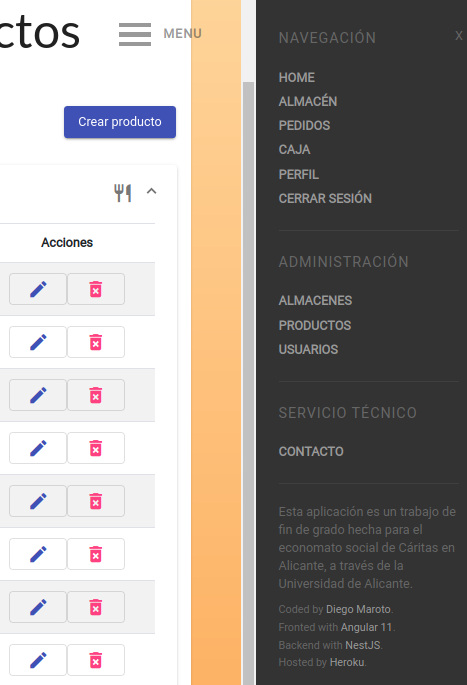
\includegraphics[scale=0.8]{archivos/decision_cromatica.png}
\caption{Ejemplo colores de la aplicación}
\label{fig:decision_cromatica}
\end{figure}
\clearpage

\subsection{Login}
\begin{figure}[h]
\centering
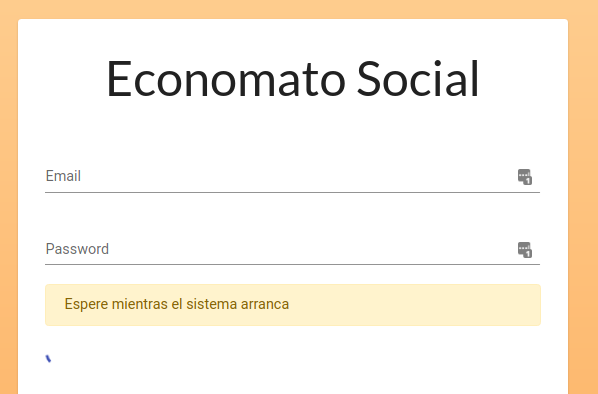
\includegraphics[scale=0.7]{archivos/login-esperando-backend.png}
\caption{Login esperando respuesta del backend}
\label{fig:login_esperando_backend}
\end{figure}
\vspace{1em}
\par En esta figura se muestra cómo el frontend, para evitar frustración del usuario, avisa de que el backend aún tienen que arrancar y debe esperar. Esto es dado por tener el frontend y el backend alojados de forma independiente y habiendo usando heroku como hosting.
\vspace{1em}
\par En heroku cuando la aplicación no recibe peticiones en 5 minutos, muere, esto hace que la siguiente petición tarde más en responder, dado que debe arrancar el sistema; Pudiendo tardar entre 20 segundos y un minuto. Esta pantalla es la que el primer voluntario que acceda a la aplicación verá cada día.
\clearpage
\begin{figure}[h]
\centering
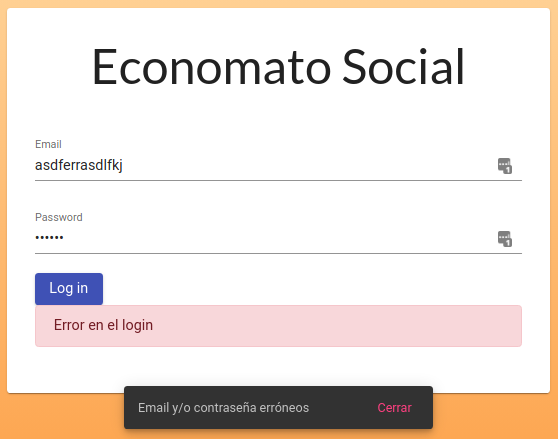
\includegraphics[scale=0.7]{archivos/login-credenciales-incorrectas.png}
\caption{Login error credenciales}
\label{fig:login_error_credenciales}
\end{figure}
\vspace{1em}
\par Este sería el comportamiento de un login incorrecto. Una posible mejora, que sería crítica en caso de ataque, sería añadir un captcha y/o un rate limiter a este tipo de vectores de ataque.
\vspace{1em}
\par Propuse añadir un rate limiter a este endpoint, dado que es el único que no requiere un jwt debidamente firmado y en vigor, pero como habían tareas más acuciantes pendientes y llegaron otras nuevas, se decidió dejar para una versión posterior.
\clearpage
\begin{figure}[h]
\centering
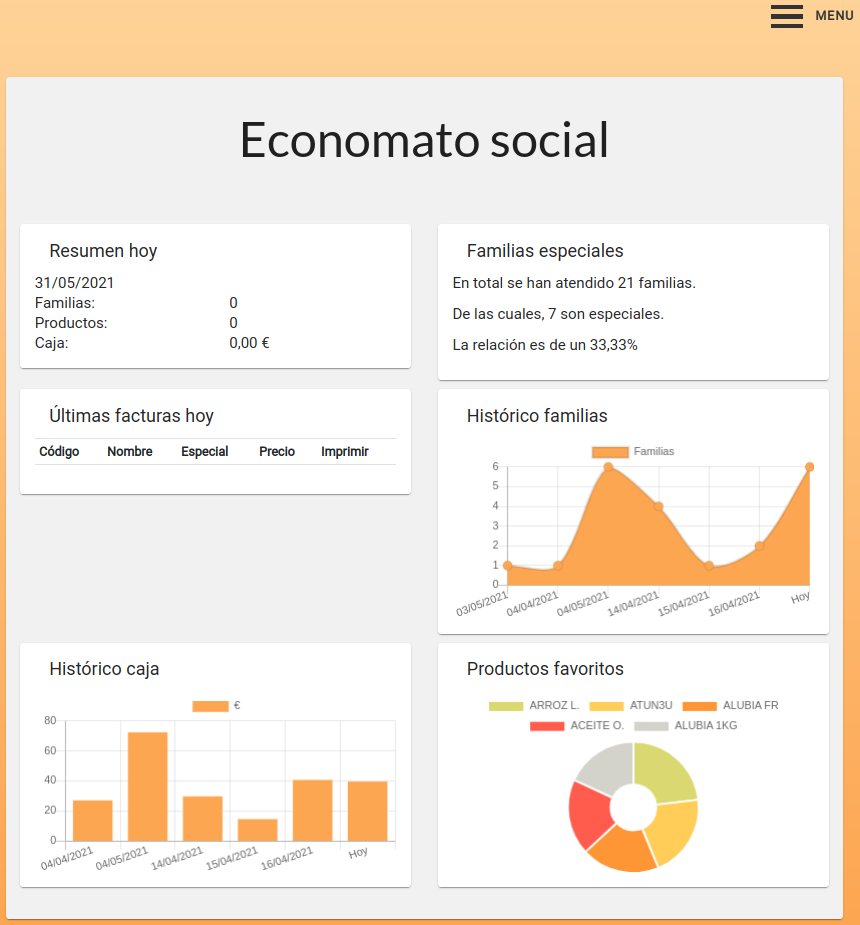
\includegraphics[scale=0.47]{archivos/dashboard.png}
\caption{Dashboard}
\label{fig:dashboard}
\end{figure}
\vspace{1em}
\par Tras un login correcto, se muestra el dashboard.
\clearpage
\subsection{Pedidos}
La sección de pedidos es un stepper, es decir, una única página que se mueve adelante y atrás de forma dinámica y a discreción del usuario y con alguna automatización. Esta sección es la que crea las facturas y para ello se obliga a que el voluntario pase por 3 subsecciones:
\begin{itemize}
    \item Búsqueda de la familia que está atendiendo, para que el sistema tenga en cuenta su histórico del mes en las restricciones de la compra
    \item La gestión de los productos que desea adquirir
    \item Resumen del pedido y generación de la factura
\end{itemize}
\vspace{1em}
\par Después de generar la factura, ésta se abre en una pestaña nueva; maquetada de forma limpia e independiente y lista para imprimir.
\begin{figure}[h]
\centering
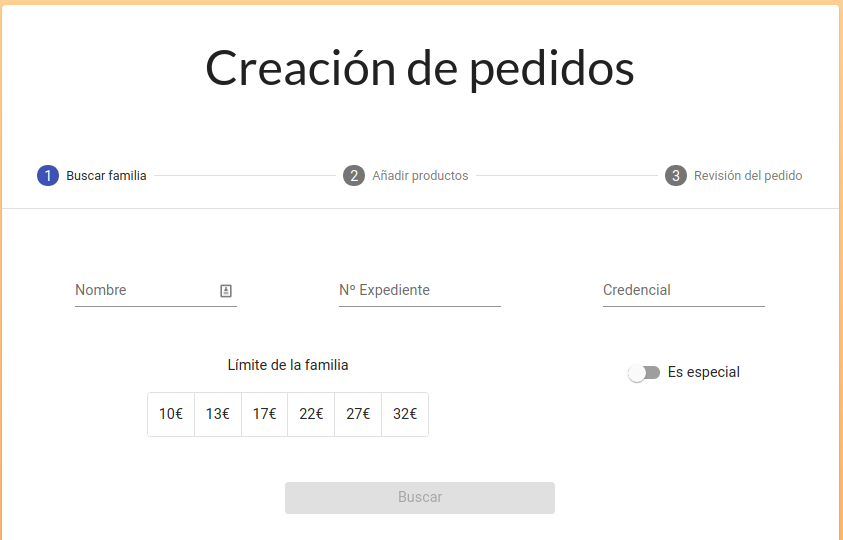
\includegraphics[scale=0.47]{archivos/pedidos-step1.png}
\caption{Pedidos: Step 1 - Búsqueda de familia}
\label{fig:pedidos_step1}
\end{figure}
\begin{figure}[h]
\centering
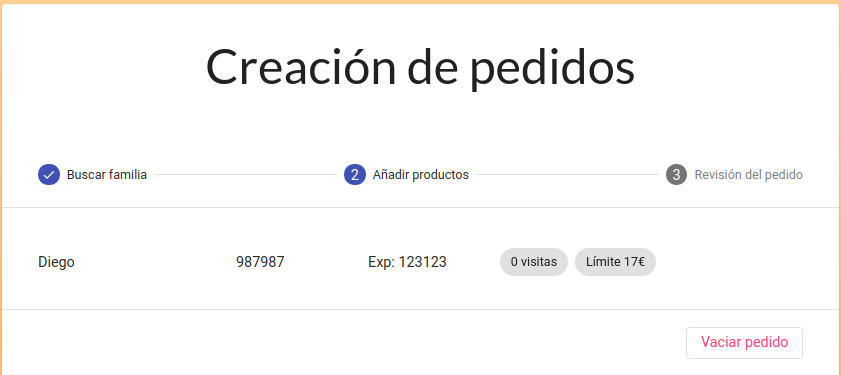
\includegraphics[scale=0.47]{archivos/pedidos-step2.png}
\caption{Pedidos: Step 2 - Resumen familia en gestión del pedido}
\label{fig:pedidos_step2_1}
\end{figure}
\begin{figure}[h]
\centering
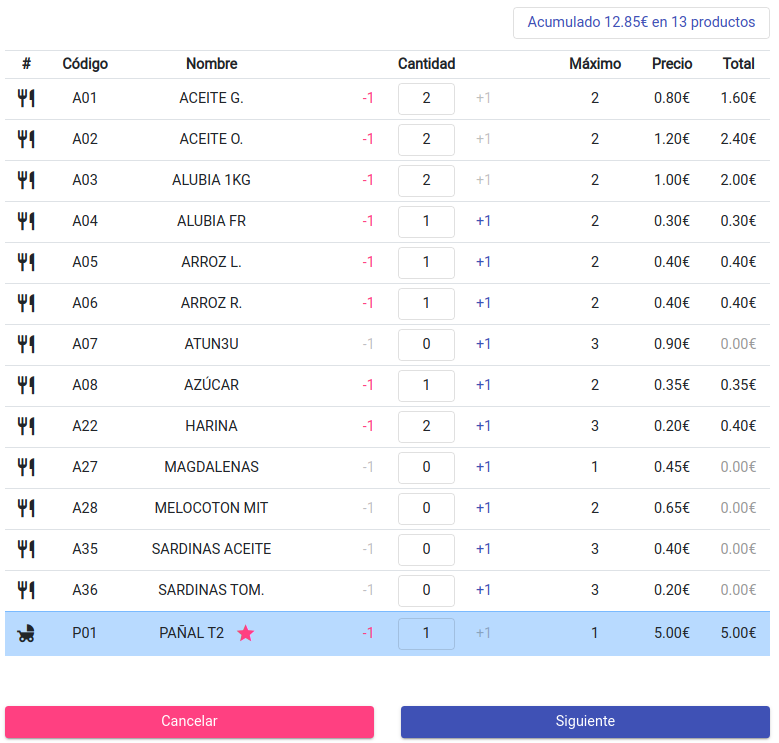
\includegraphics[scale=0.5]{archivos/pedidos-productos-resumen-botones.png}
\caption{Pedidos: Step 2 - Gestión del pedido}
\label{fig:pedidos_step2_2}
\end{figure}
\clearpage
\begin{figure}[h]
\centering
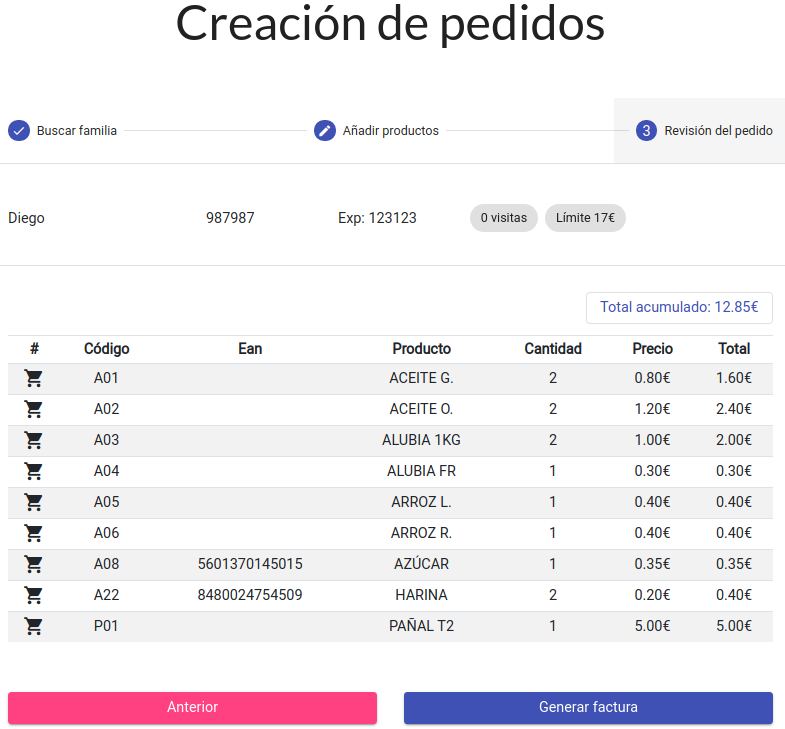
\includegraphics[scale=0.47]{archivos/pedidios-step3.png}
\caption{Pedidos: Step 3 - Resumen del pedido}
\label{fig:pedidos_step3}
\end{figure}
\clearpage
\begin{figure}[h]
\centering
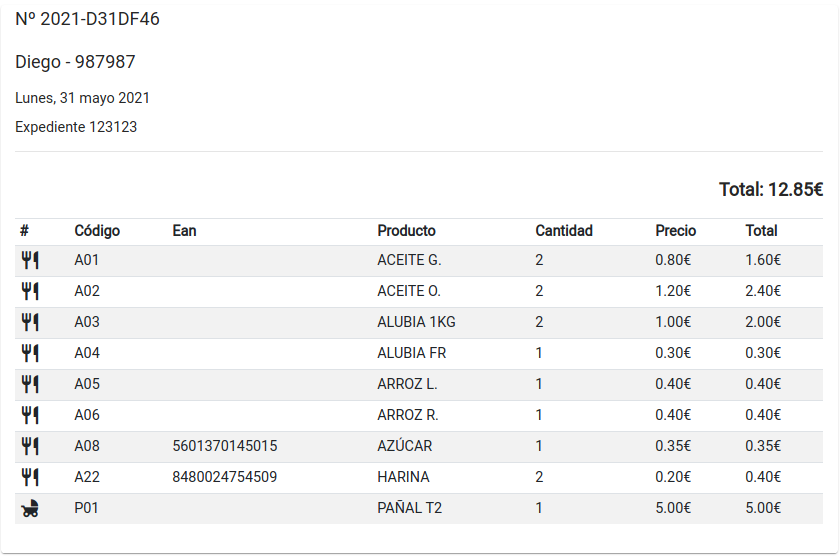
\includegraphics[scale=0.47]{archivos/maquetacion-factura.png}
\caption{Pedidos: Vista previa factura}
\label{fig:pedidos_invoice_preview}
\end{figure}
\clearpage
\begin{figure}[h]
\centering
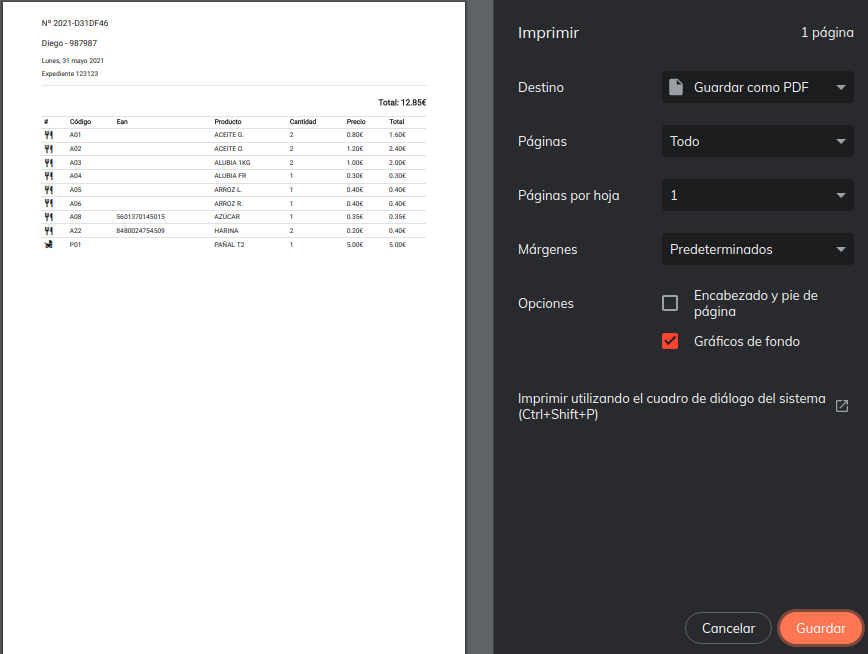
\includegraphics[scale=0.47]{archivos/imprimir-factura.png}
\caption{Pedidos: Imprimir factura}
\label{fig:pedidos_invoice_print}
\end{figure}
\clearpage
\subsection{Caja}
La sección de caja es un conjunto de acordeones que se complementan entre sí para mostrar las facturas abiertas, cobradas y cerradas (anuladas) y, por último, un resumen de caja.
\vspace{1em}
\par Las facturas que se muestra, por defecto son del día en curso, pero se puede cambiar el rango de fechas para consultar otras facturas. Además, en caso de que el usuario sea administrador, éste podrá anonimizar las facturas que se estén incluidas en el rango de fechas especificado.

\begin{figure}[h]
\centering
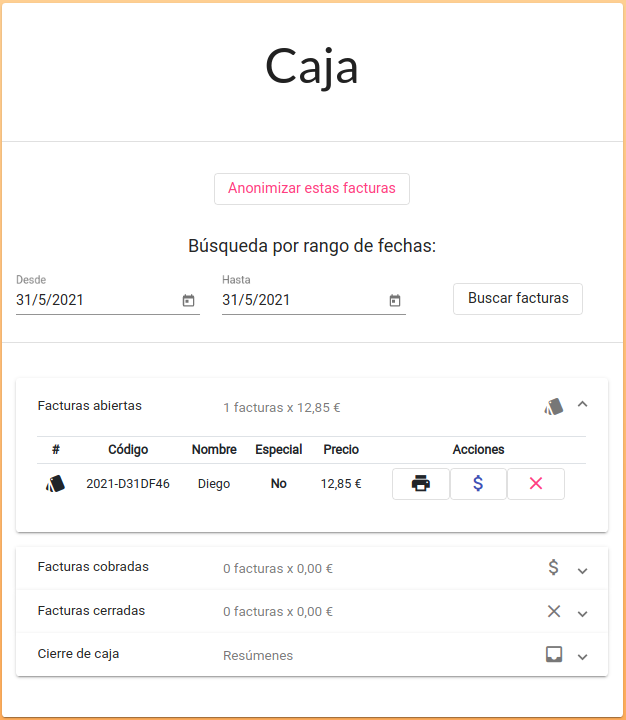
\includegraphics[scale=0.47]{archivos/caja.png}
\caption{Caja}
\label{fig:caja}
\end{figure}
\clearpage

\subsection{Almacén}
La sección de almacén es un conjunto de acordeones que se complementan entre sí para mostrar los pedidos sin despachar.
\vspace{1em}
\par Cuando se quiere despachar un pedido, aparecerá un listado de sus productos con la capacidad de marcarlos para saber si se ha preparado ya o no, esta funcionalidad se ha realizado a petición expresa de voluntarios de almacén del banco de alimentos al que se entregará el proyecto.

\begin{figure}[h]
\centering
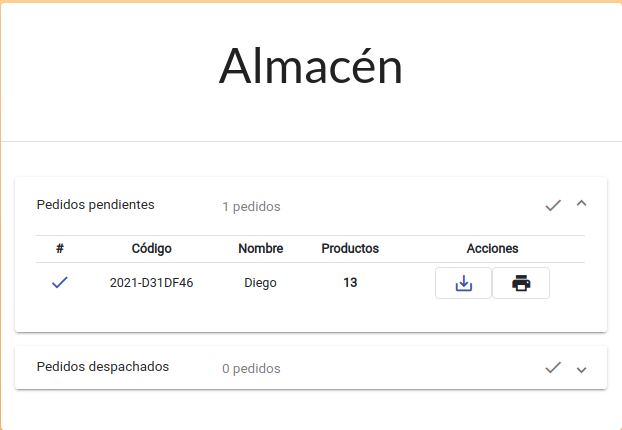
\includegraphics[scale=0.5]{archivos/almacen_1.png}
\caption{Almacén - Resumen de pedidos por despachar}
\label{fig:almacen_resumen}
\end{figure}

\begin{figure}[h]
\centering
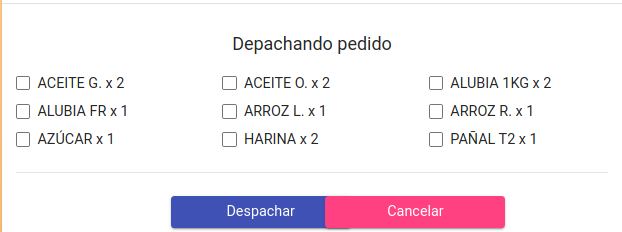
\includegraphics[scale=0.5]{archivos/almacen_2.png}
\caption{Almacén - Despachando un pedido}
\label{fig:almacen_despachando}
\end{figure}
\clearpage

\section{Implementación}
En este apartado se detallarán implementaciones que tengan relevancia en el desarrollo del proyecto, dándole un trasfondo y sentido a las pantallas que se acaban de mostrar.

\subsection{Base de datos}
Para la realización de este proyecto se ha decidido trabajar con una base de datos no relacional, en concreto con MongoDB que es una base de datos basada en documentos. Usar MongoDB como motor de base de datos ha venido especialmente bien al proyecto pues, además de usar JSON como esquema base de los documentos, hemos podido usar Compass y su capa gratuita de cluster en la nube.

\begin{lstlisting}[caption={Inyección proveedores ddbb},label=cod:ddbb-providers-injection]
export const databaseProviders = [
  {
    provide: 'MONGODB_CONNECTION',
    imports: [ConfigModule],
    inject: [ConfigService, Logger],
    useFactory: (
      configService: ConfigService<AppConfig>,
      logger: LoggerService,
    ): Promise<typeof mongoose> => {
      logger.log('CONNECTION MADE', 'ProvidersModule');
      return mongoose.connect(configService.get('mongoUrl'), {
        useNewUrlParser: true,
        useUnifiedTopology: true,
      });
    },
  },
];
\end{lstlisting}
\vspace{1em}
\par Dado que para el buen funcionamiento de la aplicación nos había solicitado atomizar los permisos que tiene cada usuario para acceder a los datos, se decidió hacer un mapa que incluye una relación entre el rol que se requiere y la lista de roles que podría tener el usuario para que el permiso fuese concedido. Por ejemplo, para realizar acciones de almacén, se debe tener cualquiera de los roles relacionados, que en esta caso son cualquiera de los 3 de administrador ó el propio de almacén. Este cruce se ideó con el pensamiento a futuro de que la aplicación pudiese crecer, complicarse los permisos y que hubiese algunos que colisionasen, por ejemplo, un permiso que fuese imprimir facturas y que éste fuese únicamente permitido a administradores, caja y pedidos; con esta implementación sólo habría que añadir un nuevo elemento al mapa con los permisos permitidos y toda la aplicación se vería afectada inmediatamente.
\clearpage
\begin{lstlisting}[caption={Gestión de roles para acceder a datos},label=cod:ddbb-roles]
export class Role {
  static permissionMap: RolePermissionMap;
  static initPermissionMap(): void {
    const map = new Map<RoleName, RoleName[]>();
    map.set(RoleName.SUPERADMIN, [RoleName.SUPERADMIN]);
    map.set(RoleName.ADMIN, [RoleName.SUPERADMIN, RoleName.ADMIN]);
    map.set(RoleName.ADMINLOCAL, [
      RoleName.SUPERADMIN,
      RoleName.ADMIN,
      RoleName.ADMINLOCAL,
    ]);
    map.set(RoleName.ALMACEN, [
      RoleName.SUPERADMIN,
      RoleName.ADMIN,
      RoleName.ADMINLOCAL,
      RoleName.ALMACEN,
    ]);
    map.set(RoleName.RECEPCION, [
      RoleName.SUPERADMIN,
      RoleName.ADMIN,
      RoleName.ADMINLOCAL,
      RoleName.RECEPCION,
    ]);
    map.set(RoleName.FAMILIAR, [
      RoleName.SUPERADMIN,
      RoleName.ADMIN,
      RoleName.ADMINLOCAL,
      RoleName.FAMILIAR,
    ]);
    map.set(RoleName.CAJA, [
      RoleName.SUPERADMIN,
      RoleName.ADMIN,
      RoleName.ADMINLOCAL,
      RoleName.CAJA,
    ]);
    Role.permissionMap = map;
  }
  static hasNeededRole(input: RoleName[], needed: RoleName): boolean {
    if (!Role.permissionMap) {
      Role.initPermissionMap();
    }
    const allowed = Role.permissionMap.get(needed);
    return allowed && input.some((role) => allowed.includes(role));
  }
}
\end{lstlisting}
\clearpage

\subsection{Esquemas y servicios}
\subsubsection{Login y registro}
\begin{lstlisting}[caption={User schema},label=cod:ddbb-user-schema]
export type UserDocument = User & Document;

export class UserComment {
  @Prop() author: string;
  @Prop() comment: string;
}

export class UserAction {
  @Prop() date: Date;
  @Prop() action: string;
}

@Schema()
export class User {
  @Prop() name: string;
  @Prop() email: string;
  @Prop() password: string;
  @Prop() active: boolean;
  @Prop() permissions: RoleName[];
  @Prop() warehouses: string[];
  @Prop() accessHistory: Date[];
  @Prop() actionsHistory: UserAction[];
  @Prop() comments: UserComment[];

  constructor(o: User) {
    Object.assign(this, o);
  }

  static fromUserDto(user: UserDto): User {
    return new User({
      name: user.name,
      email: user.email,
      active: user.active,
      permissions: user.permissions.map((p: RoleName) => p),
      warehouses: user.warehouses.map((w: string) => w),
      accessHistory: user.accessHistory.map((h: string) => new Date(h)),
      actionsHistory: user.actionsHistory.map((h: UserActionDto) => ({
        action: h.action,
        date: new Date(h.date),
      })),
      comments: user.comments.map((c: UserCommentDto) => ({
        author: c.author,
        comment: c.comment,
      })),
    });
  }
}

export const UserSchema = SchemaFactory.createForClass(User);
\end{lstlisting}

\vspace{1em}
\par El documento usuario contiene su propia contraseña, la cual está resumida con bcrypt y 10 rondas, veamos cómo se crea un usuario y cómo se hace login:
\vspace{1em}
\par 
\begin{lstlisting}[caption={Creación de un usuario},label=cod:service-user-creation]
@Injectable()
export class UserService {
  private hashRounds = 10;

  async createUser(input: UserDto): Promise<UserDto> {
    this.userValidations(input);
    const repeated: UserDocument = await this.userMongo.findOneBy(
      'email',
      input.email,
    );
    if (repeated)
      throw new ConflictException(`The email ${input.email} is in use`);
    input.password = hashSync(input.password, this.hashRounds);
    const user = User.fromUserDto(input);
    return UserService.userMapper(await this.userMongo.create(user));
  }
}
\end{lstlisting}
\vspace{1em}
\par 
\begin{lstlisting}[caption={Login de un usuario},label=cod:service-user-login]
@Injectable()
export class LoginService {
  private genericErrorMessage = 'Login error';

  async login(input: LoginDto): Promise<UserDto> {
    const user = (await this.userMongo.findBy('email', input.email))[0];
    if (!user) throw new ForbiddenException(this.genericErrorMessage);
    if (!compareSync(input.password, user.password))
      throw new ForbiddenException(this.genericErrorMessage);
    if (!user.active) {
      user.actionsHistory.push({
        date: new Date(),
        action: 'Attempt to login when inactive',
      });
      await user.save();
      throw new ForbiddenException(this.genericErrorMessage);
    }
    user.accessHistory.push(new Date());
    await user.save();
    return UserService.userMapper(user);
  }
}
\end{lstlisting}
\vspace{1em}
\par El mapeo de salida de un usuario limpia datos sensibles, en este caso es exclusivamente la contraseña.
\clearpage

\subsubsection{Productos}
El documento de productos contiene los datos necesarios para identificarlos correctamente, además de aquellos datos relacionados con OpenFoodFacts. Cada producto está relacionado con su almacén, por lo que almacenes con el mismo producto tendrán duplicidad de datos, algunos innecesarios, como los nutricionales. Una posible mejora sería sacar datos nutricionales a una colección distinta y relacionarlos por ean para evitar duplicidad, como ahora mismo sólo se tiene vista a usar un único almacén, ésta implementación se decidió dejar para versiones posteriores.
\vspace{1em}
\par 
\begin{lstlisting}[caption={Esquema de producto},label=cod:ddbb-product-schema]
export type ProductDocument = Product & Document;

export class ProductLimits {
  @Prop() price: number;
  @Prop() quantity: number;
}

@Schema()
export class Product {
  @Prop() ean: string;
  @Prop() name: string;
  @Prop() alias: string;
  @Prop() quantity: string; // amount or weight
  @Prop() categories: string;
  @Prop() ingredients: string;
  @Prop() allergens: string;
  @Prop() labels: string;
  @Prop() imageUrl: string;
  @Prop() limits: ProductLimits[];
  @Prop() pvp: number;
  @Prop() code: string; // Inner code for every warehouse
  @Prop() type: string;
  @Prop() chargeableOutBudget: boolean;
  @Prop() warehouse: string;

  constructor(o: Product) {
    Object.assign(this, o);
  }
}

export const ProductSchema = SchemaFactory.createForClass(Product);
\end{lstlisting}
\clearpage
\vspace{1em}
\par Veamos cómo se crea un producto y, en caso de tener EAN, se consulta con el api pública de OpenFoodFacts para recuperar los datos nutricionales de éste.
\begin{lstlisting}[caption={Product service: Añadir producto nuevo},label=cod:service-product-create-product]
@Injectable()
export class ProductService {
  private openFoodUrl =
    'https://world.openfoodfacts.org/api/v0/product/{{ean}}.json';
  async create(
    input: CreateProductResponseDto,
  ): Promise<ReadProductResponseDto> {
    let product = {} as Product;
    product.alias = input.alias;
    product.limits = input.limits;
    product.pvp = input.pvp;
    product.code = input.code;
    product.type = input.type;
    product.chargeableOutBudget = input.chargeableOutBudget;
    product.ean = input.ean;
    let openFoodResponse = {};
    if (product.ean)
        openFoodResponse = await this.readByEan(product.ean);
    product = {
      ...ProductService.fromOpenFoodToProduct(openFoodResponse),
      ...product,
    };
    return ReadProductResponseDto.fromProductDocument(
      await this.productsMongo.create(product),
    );
  }
  async readByEan(ean: string): Promise<any> {
    const response: AxiosResponse = await this.httpClient
      .get(this.openFoodUrl.replace('{{ean}}', ean), {
        headers: { 'User-Agent': this.config.get('openFoodUserAgent') },
      }).toPromise();
    if (!response.data.product)
      throw new InternalServerErrorException('Error requesting to openfood');
    return response.data.product;
  }
  private static fromOpenFoodToProduct(response: any): Product {
    return {
      name: response.product_name_es || response.product_name,
      ean: response.code,
      quantity: response.quantity,
      categories: response.categories,
      labels: response.labels,
      allergens: response.allergens,
      ingredients: response.ingredients_text_es || response.ingredients_text,
      imageUrl: response.image_front_url,
    } as Product;
  }
}
\end{lstlisting}
\clearpage

\subsubsection{Pedidos}
El documento de pedidos contiene los datos que hacen falta para dar completa funcionalidad a lo que se nos pidió que era necesario para procesar los pedidos de las familias.
\vspace{1em}
\par Una de las claves, es que aparecen varios identificadores de usuario, dado que es un sistema muy centrado en permitir quién puede hacer qué, es necesario almacenar quién ha hecho qué; en este caso, quién ha creado el pedido, quién lo ha cobrado y quién lo ha despachado, además de cuándo se han realizado estas acciones.
\vspace{1em}
\par Dado que la información sobre las familias está almacenada, mantenida y expedida por Cáritas, en este documento se relaciona el pedido con el documento identificativo de la familia y su expediente de Cáritas, no almacenamos datos de ningún tipo en ninguna otra colección, dado que no se sabía si tendríamos permiso, además, no resulta necesario para dar ninguno de los servicios propuestos. Esta forma de relacionar cada pedido con la familia origen, facilitó la búsqueda de qué familias han hecho visitas el mes en curso (por las restricciones) y, además, la anonimización de los pedidos, pues únicamente hay que vaciar esos campos en los pedidos del rango de fechas que se especifica en la llamada.
\vspace{1em}
\par Uno de los quebraderos de cabeza que se tuvo en el proyecto hasta llegar a este esquema final, fue que en principio se quería restringir los pedidos cuando las familias ya habían superado sus límites, pero en las reuniones de sprint en el economato llegamos a saber que habían problemas de colisión entre expedientes y documentos de identificación, que debían resolver personalmente llamando por teléfono a la sede de Cáritas. Por lo que acabamos haciendo el sistema flexible a las colisiones en este sentido y, si se revisan los vídeo-tutoriales adjuntos, se podrá apreciar que en caso de una colisión es el voluntario el que puede decidir manualmente si esta colisión afecta o no a los límites que impone el sistema.
\vspace{1em}
\par Además de lo anterior, dado que las órdenes es algo que se está consultando continuamente por diferentes secciones de la aplicación, se incluyó caché en la misma aplicación, de ésta forma salvo que la lista de pedidos del día corriente cambie, siempre que se consulten se devolverá el caché en lugar de acceder a base de datos. De ésta forma ahorramos ancho de banda y, si fuese una capa de pago, coste por procesamiento y transferencia de las consultas innecesarias.
\vspace{1em}
\par Estas peticiones tan repetitivas fue sacada a la luz por una necesidad que apareció conforme iba creciendo la aplicación, hay diferentes pantallas desde donde se está esperando que el listado de pedidos se actualice y, además, pueden ser diferentes personas/dispositivos las que estén a espensas de estos cambios. Así, pues, se hizo uso de la tecnología de websockets para poder comunicar en tiempo real cambios en los pedidos, ya sea una adición nueva, un cobro, una cancelación o haberlo despachado. Si se revisan los vídeo-tutoriales adjuntos se podrá apreciar cómo un usuario recibe en tiempo real los cambios ejecutados por otro en otro navegador.
\clearpage
Veamos el esquema de los pedidos:
\begin{lstlisting}[caption={Esquema de pedido},label=cod:ddbb-order-schema]
export type OrderDocument = Order & Document;

export class ProductResume {
  @Prop() id: string;
  @Prop() ean: string;
  @Prop() code: string;
  @Prop() name: string;
  @Prop() amount: number;
  @Prop() pvp: number;
}

@Schema({ strict: false })
export class Order {
  @Prop({ index: true }) code: string; // Code for easy human identification
  @Prop() headquarter: string; // foreign key headquarter collection
  @Prop() familyName: string;
  @Prop({ index: true }) expedient: string;
  @Prop({ index: true }) credential: string;
  @Prop() special: boolean;
  @Prop() products: ProductResume[]; // list of products
  @Prop() pvp: number;
  @Prop() type: string;
  @Prop() chargeableOutBudgetSelected: boolean;
  @Prop() createdAt: Date;
  @Prop() updatedAt: Date;
  @Prop() paid: boolean;
  @Prop() deleted: boolean;
  @Prop() origin: string; // USER ID
  @Prop() resolver: string; // USER ID
  @Prop() resolvedAt: Date;
  @Prop() dispatcher: string; // USER ID
  @Prop() dispatched: boolean;
  @Prop() dispatchedAt: Date;
}

export const OrderSchema = SchemaFactory.createForClass(Order);
\end{lstlisting}
\clearpage
\vspace{1em}
\par La creación de pedidos es una de las implementaciones que hace uso de los websockets, pues hay secciones de la aplicación que deben actualizarse en tiempo real cuando aparecen nuevos datos. Veamos cómo se ha resuelto esto:
\begin{lstlisting}[caption={Invoice service: Crear nuevo pedido},label=cod:service-invoice-create-order]
@Injectable()
export class InvoiceService {
  async create(input: Order, jwt: JWToken): Promise<any> {
    input.createdAt = new Date();
    input.updatedAt = new Date();
    input.code = `${new Date().getFullYear().toString()}-${uid(7).toUpperCase()}`;
    input.paid = false;
    input.deleted = false;
    input.origin = jwt.id;
    const order: OrderDocument = await this.mongo.create(input);
    this.broadcastInvoiceResolved(order.id, ResolveInvoiceAction.CREATED);
    await this.saveUserAction(jwt,`Invoice ${order.id} created by ${order.id}`,);
    await this.refreshCache();
    return order.toObject();
  }
  private broadcastInvoiceResolved(
    invoiceId: string,
    action: ResolveInvoiceAction,
  ): void {
    this.wsService.broadcastInvoice({ invoiceId, action });
  }
}
\end{lstlisting}
\begin{lstlisting}[caption={Websocket service: Difusión de mensajes},label=cod:service-websocket-broadcast]
@Injectable()
@WebSocketGateway()
export class WebsocketsService
  implements OnGatewayConnection, OnGatewayDisconnect {
  private wsClients: any[] = [];
  broadcastInvoice(message: InvoiceMessage): void {
    const data: WsInvoiceMessage = { event: WsTopics.INVOICES, data: message };
    this.broadcast(data, { id: null } as Socket);
  }
  broadcast(message: WsMessage | string, sender: Socket): void {
    const payload: WsMessage = { event: WsTopics.UNKNOWN, data: '' };
    if (typeof message === 'string') payload.data = message;
    else {
      payload.event = message.event;
      payload.data = message.data;
    }
    for (const c of this.wsClients) {
      if (c.id === sender.id) return;
      c.send(JSON.stringify(payload));
    }
  }
}
\end{lstlisting}
\clearpage

\subsubsection{Caja}
La gestión de caja hace uso del documento de pedidos, editando lo que necesita para dar funcionalidad a lo solicitado.
\vspace{1em}
\par Recordemos que la caja debe permitir dos acciones, cobrar pedidos o cerrarlos por erróneos. Ésto afectará al listado de pedidos del día corriente, por lo que debe actualizar la caché y, además, difundir el mensaje por websocket para que todos los clientes sepan que ha habido un cambio.
\vspace{1em}
\par Ésta implementación es susceptible de mejora, ahora mismo cuando el servidor cambia un pedido, actualiza la caché y avisa por difusión a los clientes de que ha habido un cambio, esto provoca que inmediatamente haya un aluvión de solicitudes para recuperar la lista de pedidos actualizada. Dado que está cacheada, el servidor tan cual recibe la solicitud despacha los datos directamente de la ram, sin pasar por base de datos, pero aún así, es ineficiente; sobretodo si hay muchos clientes conectados. La mejora podría consistir en difundir el nuevo estado del pedido con su identificador, de ésta forma, los clientes pueden actualizar ese pedido en concreto en sus datos locales sin más. Dado que todo lo relacionado con esta funcionalidad no era una necesidad y se hizo como mejora, se decidió que este último punto se delegase a versiones futuras, ya que impactaría en la forma en la que se difunden los mensajes y en la que los clientes deciden qué hacer con éstos.
\clearpage
Veamos la sección de código en la que se cambia el estado de un pedido de pendiente a cobrado/cerrado:
\vspace{1em}
\par 
\begin{lstlisting}[caption={Invoice service: Resolver pedido},label=cod:service-invoice-resolve-order]
export enum ResolveInvoiceAction {
  CLOSE,
  PAY,
  CREATED,
}
@Injectable()
export class InvoiceService {
  async resolveInvoice(
    id: string,
    action: ResolveInvoiceAction,
    jwt: JWToken,
  ): Promise<void> {
    const order: OrderDocument = await this.mongo.findById(id);
    if (!order) throw new NotFoundException(`Invoice with id ${id} not found`);
    if (order.paid || order.deleted) {
      throw new PreconditionFailedException('This invoice is already resolved');
    }
    switch (action) {
      case ResolveInvoiceAction.CLOSE:
        order.deleted = true;
        break;
      case ResolveInvoiceAction.PAY:
        order.paid = true;
        break;
      default:
        throw new InternalServerErrorException('Action against invoice not implemented');
    }
    this.broadcastInvoiceResolved(id, action);
    order.updatedAt = new Date();
    order.resolvedAt = new Date();
    order.resolver = jwt.id;
    await order.save();
    await this.saveUserAction(
      jwt,
      `Invoice ${order.id} updated by ${jwt.id} with action ${action}`,
    );
    await this.refreshCache();
  }
}
\end{lstlisting}
\clearpage

\subsubsection{Almacén}
La gestión de almacén también hace uso del documento de pedidos, editando lo que necesita para dar funcionalidad a lo solicitado.
\vspace{1em}
\par De una forma similar a la caja, el almacén tiene una funcionalidad muy concreta, ésta es despachar pedidos y nada más. Como bien se estuvo comentando antes, esto cambia el listado de órdenes del día y refrescará caché además de difundir el mensaje por websocket.
\vspace{1em}
\par 
\begin{lstlisting}[caption={Invoice service: Despachar pedido},label=cod:service-invoice-dispatch-order]
@Injectable()
export class InvoiceService {
  async dispatchOrder(id: string, jwt: JWToken): Promise<OrderDocument> {
    const order: OrderDocument = await this.mongo.findById(id);
    if (!order) throw new NotFoundException(`Invoice with id ${id} not found`);
    if (order.dispatched)
      throw new PreconditionFailedException('This order has been dispached already');
    order.dispatched = true;
    order.dispatcher = jwt.id;
    order.dispatchedAt = new Date();
    order.updatedAt = new Date();
    await order.save();
    await this.saveUserAction(jwt, `Order ${order.id} dispatched by ${jwt.id}`);
    this.deleteCache();
    return order;
  }
}
\end{lstlisting}
\clearpage

\subsubsection{Roles y controladores}
Por último, se procede a explicar cómo se han implementado la salvaguarda de roles en Nestjs, y dónde y cómo afecta a la aplicación.
\vspace{1em}
\par Como ya se ha comentado, uno de los requisitos indispensables es la gestión de roles de forma atómica, con solape o sin él, para manejar los permisos de los usuarios lo más estrictamente posible. De esta forma, se optó por un patrón de seguridad que se inició en los sistemas linux y se puso muy de moda en la gestión de usuarios en los servicios de infraestructura cloud. Éste es el del permiso más restrictivo por defecto, es decir, no se tendrá acceso a no ser que explícitamente se diga lo contrario.
\vspace{1em}
\par Para poder simular este patrón en el proyecto, hicimos 2 implementaciones haciendo uso del patrón Guard de Nestjs, éste viene a ser un servicio que se ejecuta antes de cualquier solicitud y que decide si se tiene acceso o no a ese recurso. Para este proyecto hay 2 guards, haciendo su magia respectivamente, en función de:
\begin{itemize}
    \item Token Bearer con un Json Web Token
    \item Roles permitidos en la ruta
\end{itemize}
\vspace{1em}
\par Su uso en Nestjs sería el siguiente:
\begin{lstlisting}[caption={User Controller: Guards en el controlador de usuario},label=cod:controller-user-guards]
@Controller('user')
@UseGuards(JwtGuard, RolesGuard)
export class UserController {
  constructor(private service: UserService) {}
  
  @Get('/:id')
  @Roles(RoleName.OWNER, RoleName.ADMINLOCAL)
  async readUserById(@Param('id') id: string): Promise<UserDto> {
    const result: UserDto = await this.service.readUserById(id);
    return result;
  }
}
\end{lstlisting}
\vspace{1em}
\par Mediante estos decoradores damos lógica automáticamente a esta clase, se convierte en un controlador de la ruta '/user' para el servidor web en Express, hace uso a nivel de controlador de los 2 guards y, en la ruta '/:id', escribe expresamente qué roles son necesarios para acceder a esa ruta.
\clearpage
El orden de los guards es importante, primero se debe manejar el jwt ya que ahí está incluído el identificador del usuario y, entre otros datos, su lista de permisos.
\begin{lstlisting}[caption={Guard JWT: Verificación de un json web token e inyección de datos en la request},label=cod:guard-jwt]
@Injectable()
export class JwtGuard implements CanActivate {
  constructor(private configService: ConfigService<AppConfig>) {}
  canActivate(context: ExecutionContext): Promise<boolean> {
    const req: Request = context.switchToHttp().getRequest();
    const bearer: string = req.header('Authorization');
    let token: JWToken;
    try {
      const regex = /^bearer (.+)$/i;
      const g = regex.exec(bearer);
      token = jwt.verify(g[1], this.configService.get('jwtSecret'));
    } catch (err) {
      throw new UnauthorizedException('Bad bearer token');
    }
    req['jwt'] = token;
    return true;
  }
}
\end{lstlisting}
\vspace{1em}
\par Este guard por defecto siempre devuelve true, ya que el único caso en el que debería impedir pasar es cuando el jwt no se puede verificar (no coincide el secreto de la firma o ha caducado), caso en el que se lanza una excepción más intuitiva. Dado que los datos extraídos del jwt deber ser accesibles más adelante, es común en Express pasar información entre middlewares inyectándolos directamente en la request, tal y como se hace en la línea 15 del código \ref{cod:guard-jwt}.
\vspace{1em}
\par Una vez verificada la identidad del usuario, se procede a revisar su rol, pasando por la implementación del guard de roles:
\begin{lstlisting}[caption={Guard Roles: Verificación de roles necesarios para el acceso},label=cod:guard-roles]
@Injectable()
export class RolesGuard implements CanActivate {
  constructor(private reflector: Reflector) {}
  canActivate(context: ExecutionContext): boolean {
    const roles = this.reflector.get<RoleName[]>('roles', context.getHandler());
    if (!roles) throw new InternalServerErrorException('Roles needed in route');
    const req: Request = context.switchToHttp().getRequest();
    const token: JWToken = req['jwt'];
    if (roles.includes(RoleName.OWNER)) {
      if (roles.length === 1) return req.params.id === token.id;
      if (req.params.id === token.id) return true;
    }
    return roles
      .filter((role) => role !== RoleName.OWNER)
      .some((role) => Role.hasNeededRole(token.roles, role));
  }
}
\end{lstlisting}
\clearpage
Esta implementación nos indica lo siguiente del guard de roles:
\begin{itemize}
    \item Es completamente obligatorio que la ruta que está siendo solicitada tenga el decorador de roles asignado.
    \begin{itemize}
        \item Línea 6 del código \ref{cod:guard-roles}
    \end{itemize}
    \item Si la ruta tiene un rol y es exclusivamente OWNER, no es cuestión de rol si no de ser dueño de los datos, si no se da el caso se corta el acceso.
    \begin{itemize}
        \item Línea 10 a 13 del código \ref{cod:guard-roles}
    \end{itemize}
    \item Por último, se verifica que de los roles que tiene el usuario, haya al menos uno compatible con las necesidades de la ruta.
    \begin{itemize}
        \item Línea 14 a 16 del código \ref{cod:guard-roles}
    \end{itemize}
\end{itemize}
\vspace{1em}
\par De esta forma tenemos las rutas protegidas, primero, obligando a que haya que acreditarse siempre; y segundo, obligando a que el desarrollador explícitamente indique qué permisos se deben complacer en las rutas que expone en la aplicación.
\vspace{1em}
\par A esta implementación le hace falta una mejora, ésta consistiría en asegurarse de poder hacer caducar los tokens, ahora mismo estos caducan a las 8 horas de su creación, para facilitar el trabajo de los voluntarios y no tener que estar logueando durante la jornada. El problema de ésto es que no se le puede retirar el acceso a alguien sin ir a su dispositivo a cerrar la sesión, habría que esperar a que le caduque el token.
\vspace{1em}
\par Veamos cómo se crean los tokens en el login de los usuarios:
\vspace{1em}
\par
\begin{lstlisting}[caption={Jwt service: Creación de token},label=cod:service-jwt-create]
createJwt(user: UserDto): string {
  const secret = this.configService.get('jwtSecret');
  const payload: Partial<JWToken> = {
    id: user.id,
    exp: moment().add(8, 'h').toDate().getTime(),
    roles: user.permissions,
    warehouses: user.warehouses,
  };
  return jwt.sign(payload, secret);
}
\end{lstlisting}
\clearpage

\section{Conclusiones, patrones y revisión del código}
Para terminar esta subsección, se procede a un pequeño análisis del código desarrollado, patrones utilizados y el framework elegido para mejorar la productividad.
\vspace{1em}
\par El uso del framework Nestjs ha permitido usar diferentes patrones de forma intuitiva y sin apenas codificar.
\begin{itemize}
    \item Patrón MVC clásico, con la salvedad de que la vista es mapeo e impresión de datos en json.
    \item Inyección de dependencias, Nestjs permite una configuración de módulos muy intuitiva que permite inyectar dependencias en el constructor de las clases con muy poca configuración, de esta forma la inicialización de las clases de las que depende la lógica de negocio es completamente agnóstica a la misma lógica de negocio.
    \item Patrón singleton, los servicios injectables en Nestjs que se importan desde módulos independientes tienen la peculiaridad de que sólo se instancian una vez por módulo, ahorrando memoria y errores de implementación en caso de querer hacerlo manualmente.
    \item Patrón factory, Nestjs usa una factory por defecto para crear el model de Mongodb a partir de una clase decorada como esquema. Además, en el proyecto se ha usado el patrón factory para construir los dto de salida a partir de un documento de Mongodb.
\end{itemize}
\vspace{1em}
\par Nestjs tiene muchos más beneficios, como el enrutado automático del servidor web o la configuración automática del servidor de documentación basado en swagger.
\vspace{1em}
\par Para el frontend se ha usado Angular 11, del cual se ha expuesto menos código ya que es muy similar al backend. Ésta fue una de las razones de usar la combinación Nestjs y Angular, ambos son MVC con módulos configurables e inyectables y usan una sintaxis muy similar, de ésta forma ser conocedor de uno de los dos framework hace el acercamiento al otro mucho más sencillo y con muy poca curva de aprendizaje.
\vspace{1em}
\par Para ahorrar esfuerzo y tiempo en diseño se han usado paquetes de Angular que traen animaciones y maquetaciones, Angular Material. Y para la estructuración y el responsive se ha usado Bootstrap 4, éste no es de Angular pero hay integraciones libres de la comunidad que integran a la perfección las dependencias de Bootstrap con las de Angular para hacer funcionar sin problema este framework.
\clearpage
Más allá de los frameworks, en el desarrollo del backend se ha hecho especial hincapié en desarrollar teniendo en mente los principios SOLID \citep{SOLID}:
\begin{itemize}
    \item S: Responsabilidad única.
    \begin{itemize}
        \item División del proyecto en módulos y servicios independientes, intentando siempre que cada clase y/o función se haga cargo exclusivamente de lo que le concierne.
    \end{itemize}
    \item O: Principio abierto/cerrado.
    \begin{itemize}
        \item Cuando se ha tenido que añadir o cambiar lógica, se ha intentado siempre minimizar el impacto que esto tiene sobre las funcionalidad actuales. Las factories han servido de ayuda, ya que aíslan funcionalidades concretas de forma estática e independiente de clases relacionadas. 
    \end{itemize}
    \item L: Sustitución de Liskov.
    \begin{itemize}
        \item Cuando hay herencia, las clases hijas deben servir para lo mismo que para los padres. En este proyecto se ha usado herencia de una clase abstracta para dar funcionalidad genérica a servicios de la capa de datos, las funcionalidad no cambian entre servicios, sólo las colecciones a las que hacen referencia.
    \end{itemize}
    \item I: Segregación de interfaces.
    \begin{itemize}
        \item Se ha intentado hacer prevalecer la alta cohesión frente al acoplamiento, la modularización de Nestjs ha ayudado en este menester.
    \end{itemize}
    \item D: Inversión de dependencias
    \begin{itemize}
        \item Principalmente en la capa de acceso a datos, se ha implementado de forma que los detalles dependen de las abstracciones y no al revés.
    \end{itemize}
\end{itemize}
\vspace{1em}
\par Para finalizar, se ha pretendido mantener el código todo lo seco posible: DRY (Don't Repeat Yourself), haciendo uso de herencias, funciones y extrayendo a módulos inyectables las codificaciones que se han detectado como generalizaciones.

\section{Resultado final}
Para finalizar este capítulo sabe señalar que hay mucho más código y muchos más detalles en la aplicacíon de lo que se puede expresar en un documento. Por lo que se va a aprovechar este cierre para incluir enlaces directamente a los servicios desplegados en producción, vídeo-tutoriales que se han entregado junto al proyecto al economato social y el enlace al proyecto en el repositorio remoto Github.
\begin{itemize}
    \item \href{https://economato-social-api.herokuapp.com}{Enlace al Backend} \citep{BACKEND}
    \item \href{ttps://economato-social.herokuapp.com}{Enlace al Frontend} \citep{FRONTEND}
    \item \href{https://github.com/DiegoMGar/TFG}{Enlace al Repositorio público en Github}  \citep{REPOSITORIO}
    \item \href{https://drive.google.com/drive/folders/1pv-6iishQkM29StiSHUyY74lWEVx0t6q}{Enlace a los Vídeo-tutoriales} \citep{VIDEOTUTORIALES}
\end{itemize}
		% Plantilla: Se muestran listados
%%%%%%%%%%%%%%%%%%%%%%%%%%%%%%%%%%%%%%%%%%%%%%%%%%%%%%%%%%%%%%%%%%%%%%%%
% Plantilla TFG/TFM
% Escuela Politécnica Superior de la Universidad de Alicante
% Realizado por: Jose Manuel Requena Plens
% Contacto: info@jmrplens.com / Telegram:@jmrplens
%%%%%%%%%%%%%%%%%%%%%%%%%%%%%%%%%%%%%%%%%%%%%%%%%%%%%%%%%%%%%%%%%%%%%%%%

\chapter{Resultados (Con ejemplos de gráficos)}
\label{resultados}

\section{Diagramas}
Gracias al paquete \textit{Tikz} se pueden incluir multitud de medios gráficos, diagramas, capas sobre imágenes, etc.
Existen múltiples formas de realizarlo, para ello es recomendable consultar la guía de iniciación disponible aquí: \url{http://cremeronline.com/LaTeX/minimaltikz.pdf} y también el manual completo disponible aquí: \url{http://osl.ugr.es/CTAN/graphics/pgf/base/doc/pgfmanual.pdf}.
\\
\par A continuación se muestran algunos ejemplos. Revisa el archivo .tex para ver cómo se utilizan.
\\
\par Imagen a la que se le ha añadido cuadros y texto desde latex:
\begin{figure}[ht]
\centering	
\resizebox{0.6\textwidth}{!}{%
\begin{tikzpicture}[x=39, y=47]%X,Y -> Corrección de coordenadas, según tamaño y posición de la imagen
    \node[anchor=south west,inner sep=0] (image) at (0,0) {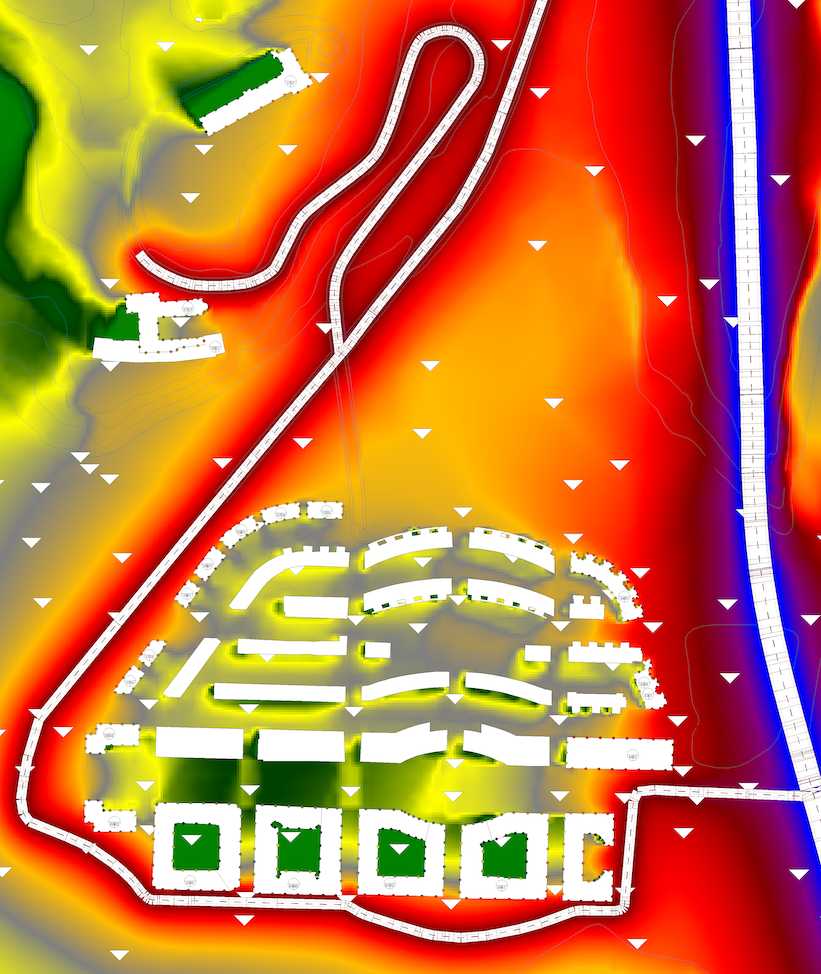
\includegraphics[width=0.9\textwidth]{archivos/mapadia}};
    % Imprimir coordenadas
    \begin{scope}[x={(image.south east)},y={(image.north west)}]
        \draw[help lines,xstep=.1,ystep=.1] (0,0) grid (1,1);
        \foreach \x in {0,1,...,9} { \node [anchor=north] at (\x/10,0) {\x}; }
        \foreach \y in {0,1,...,9} { \node [anchor=east] at (0,\y/10) {\y}; }
    \end{scope}
    % Residencias 1
    \draw[Caja1] (6.8,2) rectangle (8.3,4.5);
    \node[Texto2] at (6.8,2) {\textbf{Residencias 1}};
    % Residencias 2
    \draw[Caja1] (1,0.6) rectangle (7.6,1.8);
    \node[Texto2] at (1,0.6) {\textbf{Residencias 2}};
    % Residencias 3
    \draw[Caja1,rotate around={-45:(2.6,3.6)}] (2.6,3.6) ellipse (1cm and 3.1cm);
    \node[Texto2] at (1.2,2.1) {\textbf{Residencias 3}};
    % Hospital
    \draw[Caja1] (1,6) rectangle (3,7);
    \node[Texto2] at (1,6) {\textbf{Hospital}};
    % Colegio
    \draw[Caja1] (2.3,8.5) rectangle (3.9,9.5);
    \node[Texto2] at (2.3,8.5) {\textbf{Colegio}};
    % Numeros de edificios
    \node[Texto3,font=\tiny] at (7.5,4) {\textbf{1}};
    \node[Texto3,font=\tiny] at (7.9,2.9) {\textbf{2}};
    \node[Texto3,font=\tiny] at (7.7,2.3) {\textbf{3}};
    \node[Texto3,font=\tiny] at (7.2,1.2) {\textbf{4}};
    \node[Texto3,font=\tiny] at (6.2,1.2) {\textbf{5}};
    \node[Texto3,font=\tiny] at (4.9,1.2) {\textbf{6}};
    \node[Texto3,font=\tiny] at (3.6,1.2) {\textbf{7}};
    \node[Texto3,font=\tiny] at (2.4,1.2) {\textbf{8}};
    \node[Texto3,font=\tiny] at (1.5,1.7) {\textbf{9}};
    \node[Texto3,font=\tiny] at (1.5,2.5) {\textbf{10}};
    \node[Texto3,font=\tiny] at (1.5,3) {\textbf{11}};
    \node[Texto3,font=\tiny] at (1.8,3.4) {\textbf{12}};
    \node[Texto3,font=\tiny] at (2.2,3.8) {\textbf{13}};
    \node[Texto3,font=\tiny] at (2.5,4.2) {\textbf{14}};
    \node[Texto3,font=\tiny] at (3,4.5) {\textbf{15}};
    \node[Texto3,font=\tiny] at (3.4,4.8) {\textbf{16}};
    \node[Texto3,font=\tiny] at (4,4.8) {\textbf{17}};
    % Nombres de carreteras
    \node[Texto3] at (9.2,7) {\textbf{A-7}};
    \node[Texto3] at (9,1.8) {\textbf{N-1}};
    \node[Texto3] at (4,8) {\textbf{N-2}};
\end{tikzpicture}
}
\end{figure}

En muchas ocasiones es necesario realizar un diagrama de bloques, más abajo se muestra un ejemplo de ello. En la red hay multitud de ejemplos que pueden ser fácilmente modificables para un fin concreto, como por ejemplo en esta web: \url{http://www.texample.net/tikz/examples/tag/block-diagrams/}.
\begin{figure}[ht]
\centering 
\begin{tikzpicture}[node distance=2cm, auto]
	% Cuadros
	\node (pc) [rectvioleta,text width=3cm] {Ordenador{\\}\small{Software: ARTA} \par};
	\node (sound) [rectamarillo, below of=pc, text width=4cm] {Tarjeta de sonido {\\}Tascam US-144MKII \par};
	\node (nexus) [rectverde, right of=sound,xshift=6cm, text width=8cm] { Amplificador/Adaptador de impedancia{\\}DIY\par };
	\node (acel) [rectnaranja, below of=nexus,text width=3cm,xshift=0cm]{\small Acelerómetro {\\}Brüel {\&} Kjær TYPE 4514B-002 \par};
	\node (micro) [rectnaranja, below of=sound,text width=3cm,xshift=0cm]{\small Micrófono {\\}Behringer ECM8000 \par};
	\node (excit) [rectnaranja, below of=acel,text width=3cm,xshift=2cm]{\small Excitador \par};
	\node(barra) [romborosa, below of=acel,xshift=-3.1cm]{\small Barra \par};
	% Flechas
	\draw[arrow] (pc) -- (sound);
	\draw[arrow] (sound) -- (pc);
	\draw[arrow] (nexus) -- (sound);
	\draw[arrow] (excit) -- (barra.east);
	\draw[arrow] (micro) -- (sound);
	\draw[arrow] (barra.west) -- (0,-6)-- (micro.south);
	\draw[arrow] (barra.west) -- (3.4,-4)--(acel.west);
 	\draw[arrow] (acel) -- (nexus);	
\end{tikzpicture}
\caption{Diagrama realizado en latex con Tikz.}
\label{fig:blockcv}
\end{figure}



\section{Gráficas}

Existen múltiples formas de generar gráficas para latex. Hay disponibles herramientas como GeoGebra que dispone de la utilidad para exportar los gráficos en formato Tkiz. También funciones para Matlab que genera las gráficas que muestra habitualmente pero en código para Tkiz.

\subsection{Línea}
La forma más simple, aunque no sencilla cuando abarca muchos datos es la siguiente:

\begin{lstlisting}[style=Latex-color]
\begin{figure}[ht]
\centering
	\begin{tikzpicture}
  		\begin{axis}
  			[ymin=0,ymax=5, % Límites del eje y
  			xmin=0,xmax=6,  % Límites del eje x
  			ylabel= eje Y, 	% Nombre del eje y
    		xlabel= eje X]  % Nombre del eje x
    		\addplot+[smooth] coordinates % Une los puntos curva suavizada
      		{(0,0) (1,2) (2,3 (4,3))}; % Puntos de la gráfica
  		\end{axis}
	\end{tikzpicture}
\caption{Gráfica sencilla.}
\end{figure}
\end{lstlisting}

El resultado es el siguiente:
\\
\begin{figure}[ht]
\centering
	\begin{tikzpicture}
  		\begin{axis}
  			[ymin=0,ymax=5, 
  			xmin=0,xmax=6,
  			ylabel= eje Y,
    		xlabel= eje X]
    		\addplot+[smooth] coordinates
      		{(0,0) (1,2) (2,3) (4,3)};
  		\end{axis}
	\end{tikzpicture}
\caption{Gráfica sencilla.}
\end{figure}
\FloatBarrier

Otro ejemplo, en este caso las lineas están calculadas directamente en LaTex y después cada una tiene una anotación (el código se encuentra en el archivo archivos/ejemplos/perjudicialesopticacentro.tex):

\begin{figure}[H]
	\centering%
    \input{archivos/ejemplos/perjudicialesopticacentro}%
    \caption{OP/S003}%
\end{figure}%

\subsection{Barras}
Otro ejemplo es la gráfica de barras:
\begin{lstlisting}[style=Latex-color]
\begin{figure}[ht]
\centering
\begin{tikzpicture}
	\begin{axis}[
	    ybar=12pt,
	    ymin=0,ymax=150,
	    xtick=data,
	    enlarge x limits={abs=2cm},
	    symbolic x coords={rubio, moreno},
	    bar width = 20pt,
	    ylabel= número,
	    xlabel= color de pelo,
	        ytick align=outside,
	        ytick pos=left,
	        major x tick style = transparent,
	        legend style={at={(0.04,0.96)},anchor=north west, font=\footnotesize, legend cell align=left,},
	        ]
	    \addplot[ybar,fill=blue, area legend] coordinates {
	        (rubio,20)
	        (moreno,100)};
	    \addplot[ybar,fill=purple, area legend] coordinates {
	        (rubio,110)
	        (moreno,105)};
	 \legend{Chicos, Chicas}
	\end{axis}
\end{tikzpicture}
\caption{Gráfica barras.}
\end{figure}
\end{lstlisting}

El resultado es el siguiente:

\begin{figure}[ht]
\centering
\begin{tikzpicture}
	\begin{axis}[
	    ybar=12pt,
	    ymin=0,ymax=150,
	    xtick=data,
	    enlarge x limits={abs=2cm},
	    symbolic x coords={rubio, moreno},
	    bar width = 20pt,
	    ylabel= número,
	    xlabel= color de pelo,
	        ytick align=outside,
	        ytick pos=left,
	        major x tick style = transparent,
	        legend style={at={(0.04,0.96)},anchor=north west, font=\footnotesize, legend cell align=left,},
	        ]
	    \addplot[ybar,fill=blue, area legend] coordinates {
	        (rubio,20)
	        (moreno,100)};
	    \addplot[ybar,fill=purple, area legend] coordinates {
	        (rubio,110)
	        (moreno,105)};
	 \legend{Chicos, Chicas}
	\end{axis}
\end{tikzpicture}
\caption{Gráfica barras.}
\end{figure}
\FloatBarrier

\subsection{Polar}
Un ejemplo de gráfica polar semicircular (ver archivo archivos/ejemplos/polarnorm.tex):

\begin{figure}[H]
    	\centering%
         {\scalefont{0.8}%
    \input{archivos/ejemplos/polarnorm}%
    }
    \caption{Directividad normalizada del altavoz (0 dBV en el eje).}\label{norma}
\end{figure}


\section{Importados de MATLAB}
\label{impmatlab}
Gracias a la herramienta \textit{matlab2tikz} (\url{https://es.mathworks.com/matlabcentral/fileexchange/22022-matlab2tikz-matlab2tikz}) se pueden exportar las gráficas de cualquier tipo de Matlab a latex.
Después de incluir los archivos de \textit{matlab2tikz} se debe escribir una llamada después de crear la figura tal que:

\begin{lstlisting}[style=Matlab-color,caption={Ejemplo de llamada a matlab2tikz}]
fig = plot(x,y);
matlab2tikz('figurehandle',fig,'NombreArchivo.tex','height','5cm','width','13.5cm','strict',true,'showHiddenStrings',true,'showInfo',false)
\end{lstlisting}

Y para utilizar el archivo generado por la función en este documento:
\begin{lstlisting}[style=Latex-color]
\begin{figure}[ht]
	\centering
	{\scalefont{0.8}\input{archivos/ejemplos/ParedFina} }
	\caption{Ejemplo de gráfica obtenida con matlab2tikz.}
\end{figure}
\end{lstlisting}

\begin{figure}[ht]
	\centering
	{\scalefont{0.8}\input{archivos/ejemplos/ParedFina} }
	\caption{Ejemplo de gráfica obtenida con matlab2tikz.}
\end{figure}
\FloatBarrier
Ejemplo de una gráfica 3D generada en Matlab y exportada por \textit{matlab2tikz}:
\begin{figure}[ht]
		\centering
		{\scalefont{0.8}\input{archivos/ejemplos/2D-3314hz} }
		\caption{Amplitud de la aceleración en el modo número 8.}
\end{figure}
\FloatBarrier

\section{Ejemplo avanzado}

El potencial del paquete \textit{Tikz} es muy alto, se pueden realizar muchísimas cosas. En la red se facilitan muchos ejemplos para poder ver el funcionamiento y aprender. Existen hilos donde la gente publica sus mejores diseños de \textit{Tikz} como en \url{https://tex.stackexchange.com/questions/158668/nice-scientific-pictures-show-off} o páginas donde facilitan muchas plantillas como \url{http://www.texample.net/tikz/examples/all/}.
\par Un ejemplo de lo que se puede llegar a conseguir es el siguiente:
% Vector Styles
\tikzset{
  load/.style   = {ultra thick,-latex},
  stress/.style = {-latex},
  dim/.style    = {latex-latex},
  axis/.style   = {-latex,black!55},
}

% Drawing View
\tikzset{dimetric2/.style={
  x={(0.935cm,-0.118cm)},
  y={(0.354cm, 0.312cm)},
  z={(0.000cm, 0.943cm)},
}}
\begin{figure}[ht]
\centering
  \begin{tikzpicture}
    \node (origin) at (0,0) {}; % shift relative baseline
    \coordinate (O) at (2,3);
    \draw[fill=gray!10] (O) circle (1);
    \draw[fill=white] (O) circle (0.75) node[below,yshift=-1.125cm] {Corte trasversal};
    \draw[dim] (O) ++(-0.75,0) -- ++(1.5,0) node[midway,above] {$d_i$};
    \draw[dim] (O) ++(-1,1.25) -- ++(2,0) node[midway,above] {$d_o$}; 
    \foreach \x in {-1,1} {
      \draw (O) ++(\x,0.25) -- ++(0,1.25);
    }
  \end{tikzpicture}
  \begin{tikzpicture}[dimetric2]
        \coordinate (O) at (0,0,0);
        \draw[axis] (O) -- ++(6,0,0) node[right] {$x$};
        \draw[axis] (O) -- ++(0,6,0) node[above right] {$y$};
        \draw[axis] (O) -- ++(0,0,6) node[above] {$z$};
        \draw[fill=gray!50] (0,0,-0.5) circle (0.5); 
        \fill[fill=gray!50] (-0.46,-0.2,-0.5) -- (0.46,0.2,-0.5) -- (0.46,0.2,0) -- (-0.46,-0.2,0) -- cycle;
        \draw[fill=gray!20] (O) circle (0.5);
    \draw (0.46,0.2,-0.5) -- ++(0,0,0.5) node[below right,pos=0.0] {Soporte fijo};
    \draw (-0.46,-0.2,-0.5) -- ++(0,0,0.5);
    \draw[fill=gray!10] (O) circle (0.2);
    \fill[fill=gray!10] (-0.175,-0.1,0) -- (0.175,0.1,0) -- ++(0,0,4) -- (-0.175,-0.1,4) -- cycle;
    \draw (-0.175,-0.1,0) -- ++(0,0,4);
    \draw (0.175,0.1,0) -- ++(0,0,4) node[right,midway] {Poste de acero};
    \draw (4,0,3.95) -- ++(0,0,-1);
    \foreach \z in {0.5,0.75,...,5} {
      \draw[-latex] (-2*\z/5-0.2,0,\z) -- (-0.2,0,\z);
    }
    \draw[load] (0,0,4) -- ++(0,0,-1.25) node[right,xshift=0.1cm] {$F_{z1}$};
    \draw[fill=gray!20] (-0.25,-0.25,5) -- (4,-0.25,5) -- (4,+0.25,5) -- (-0.25,+0.25,5) -- cycle; 
    \draw[fill=gray!50] (+4.00,-0.25,4) -- (4,+0.25,4) -- (4,+0.25,5) -- (+4.00,-0.25,5) -- cycle; 
    \draw[fill=gray!10] (-0.25,-0.25,4) -- (4,-0.25,4) -- (4,-0.25,5) -- (-0.25,-0.25,5) -- cycle; 
    \draw (4.05,0,4) -- ++(1,0,0);
    \draw (4.05,0,5) -- ++(1,0,0);
    \draw[dim] (4.5,0,0) -- ++(0,0,4) node[midway,right] {$h_1$};
    \draw[dim] (4.5,0,4) -- ++(0,0,1) node[midway,right] {$h_2$};
    \draw[dim] (0,0,3.4) -- ++(4,0,0) node[midway,below] {$b_2$};
    \coordinate (P) at (2,-0.25,4.5);
    \draw (P) -- ++(0,0,0.25);
    \draw (P) -- ++(0.25,0,0);
    \draw[dim] (2.125,-0.25,4.5) -- ++(0,0,-0.5) node[midway,right] {$z_1$};
    \draw[dim] (2,-0.25,4.625) -- ++(-2,0,0) node[midway,below] {$x_1$};
    \draw[load] (2,-2.45,4.5) -- ++(0,2.2,0) node[pos=0.0,right,xshift=0.08cm] {$F_{y1}$};
    \draw[axis,dashed,-] (O) -- (0,0,5);
    \draw (0,0,5.5) -- ++(4,0,0) node[midway,above] {$w_{z}$};
    \foreach \x in {0,0.25,...,4} {
      \draw[-latex] (\x,0,5.5) -- ++(0,0,-0.5);
    }
    \draw (-0.2,0,0) -- ++(-2,0,5) node[above,xshift=0.5cm] {$w_{x}=\frac{z}{h_1+h_2} w_0$};
  \end{tikzpicture}
\caption{Señal realizada con Tikz, sin imágenes.}
\label{senyal}
\end{figure}
\FloatBarrier
		% Plantilla: Se muestran gráficas
%%%%%%%%%%%%%%%%%%%%%%%%%%%%%%%%%%%%%%%%%%%%%%%%%%%%%%%%%%%%%%%%%%%%%%%%
% Plantilla TFG/TFM
% Escuela Politécnica Superior de la Universidad de Alicante
% Realizado por: Jose Manuel Requena Plens
% Contacto: info@jmrplens.com / Telegram:@jmrplens
%%%%%%%%%%%%%%%%%%%%%%%%%%%%%%%%%%%%%%%%%%%%%%%%%%%%%%%%%%%%%%%%%%%%%%%%

\chapter{Conclusiones}
\label{conclusiones}
Una vez finalizado el proyecto, no está de mas recapitular y revisar el trabajo realizado. Es una buena forma de revisar si se han logrado cumplir los objetivos que se marcaron en un inicio.
\section{Revisión de los objetivos marcados}
Los objetivos que se pretendían conseguir son los siguientes:
\begin{itemize}
    \item Investigar y analizar soluciones hardware lowcost
    \begin{itemize}
        \item Se ha realizado un estudio de diferentes tipos de sistemas a tener en cuenta, pasando desde el self-hosting con una raspberry pi a terminar decidiendo usar servicios serverless cloud en heroku.
    \end{itemize}
    \item Investigar y analizar el estado de los bancos de alimentos en el mundo y su relación con la tecnología
    \begin{itemize}
        \item Se han investigado proyectos y necesidades, quedando patente las potenciales implicaciones positivas que tendría adoptar en mayor medida la tecnología en el campo social
    \end{itemize}
    \item Estudiar el mercado para decidir el stack tecnológico en el que desarrollar la aplicación
    \begin{itemize}
        \item Se ha realizado un estudio centrado en encuestas de StackOverflow, líder en el de la comunidad online tecnológica, para decidir lenguajes a utilizar.
    \end{itemize}
    \item Estudiar alternativas de software en el mercado
    \begin{itemize}
        \item Se ha investigado si la solución que se pretende con este proyecto podría ser solventada por uno de los CRM que ya existen en el mercado, si bien hay mucha comunidad tecnológica a penas hay proyectos libres adhoc para este tipo de necesidades.
    \end{itemize}
    \item Diseñar la aplicación web conforme a los requisitos recogidos del economato social
    \begin{itemize}
        \item Se estudiaron y documentaron los requisitos fundamentales que la aplicación debería cubrir y no sólo se han cumplido en su totalidad si no que se han implementado mejoras a lo largo del proyecto y, cuando ya se había finalizado el desarrollo, se aceptaron dos nuevas implementaciones y se llevaron a cabo en tiempo y forma.
    \end{itemize}
    \item Uso de metodología ágil con entrega continua
    \begin{itemize}
        \item Se ha adoptado con éxito una metodología ágil basada en sprints de 3 semanas, con reuniones en vivo con el economato para recoger feedback y requisitos; habiendo construido así una solución totalmente a medida.
    \end{itemize}
    \item Entregar la aplicación web en su versión acabada
    \begin{itemize}
        \item Se ha entregado la aplicación finalizada y usable desplegada en un host gratuito, además de guía de uso y vídeo tutoriales para facilitar la adopción de los voluntarios del economato social.
    \end{itemize}
\end{itemize}
\section{Conclusiones}
Para concluir esta memoria, cabe destacar que ha sido un auténtico placer desarrollar una aplicación de estas características debido al uso que se le pretende dar. Ha sido un desafío, personal y académico, tanto por el alcance del proyecto como por la situación de pandemia en la que nos encontramos. Haber sido parte de un proyecto como este hace mella en uno, saber que los conocimientos y habilidades pueden ser puestas en pos de los más necesitados y de que sólo hacen falta ganas y no grandes presupuestos para mejorar la calidad laboral de aquellos que se ponen en primera línea para ayudar a los más necesitados. Ha sido una experiencia enriquecedora y si puedo, seguiré colaborando y mejorando este proyecto a lo largo del tiempo hasta que, por la razón que sea, no me sea posible aportar nada más. Deseo que la adopción de la tecnología en el campo social no deje de crecer y que, efectivamente, algún día los bancos sociales tengan voluntarios o financiación suficiente como para que la tecnología deje de ser un muro tan insalvable como lo es hoy.
\vspace{1em}
\par Además de lo personal, profesionalmente ha sido un reto. He tenido que desempolvar conocimientos de la carrera, sacar las mejores herramientas y dar lo mejor de mí para llegar a buen puerto. No es mi primera experiencia como full-stack pero sí puedo decir sin miedo que es la primera vez que desarrollo yo sólo un proyecto de éste alcance y del que hay gente que espera tanto, me he visto necesitado de sacar a relucir patrones de diseño y conocimientos avanzados en tecnología y arquitectura cloud que he adquirido personal y profesionalmente en mis años de experiencia. Siento que ha sido una gran experiencia y que, aunque esté terminando de escribir la memoria de este proyecto, aún queda mucho por desarrollar y mejorar en la entrega que terminar aquí supone.
\vspace{1em}
\par Al principio no las tenía todas conmigo en la decisión de volcar los esfuerzos en desarrollar una solución cloud native, dado que la idea de usar el self-hosting tenía mucho peso inicial. Pero por suerte no hubo arrepentimientos, las automatizaciones hicieron su magia para facilitarme el trabajo en el CI/CD y las capas gratuitas de hosting y base de datos nos han permitido entregar un producto de calidad que funciona a coste cero y que, dada la naturaleza inicial de configuración y desarrollo, podríamos migrar a cualquier otro servicio cloud o proveedor de base de datos con muy poco esfuerzo; en caso de ser necesario.
\vspace{1em}
\par Para finalizar me gustaría comentar que aún hay mucho por recorrer en la tecnología centrada en el campo social y, con los retos que tenemos encima ahora mismo por la pandemia, seguro que hay muchísimas ideas que podemos llevar a cabo. Desarrollos y avances que no pueden hacer otra cosa que mejorar nuestra sociedad justo donde más falta hace, donde no hay recursos informáticos ni educación tecnológica.	% Plantilla: Se muestran matemáticas

%%%%
% CONTENIDO. BIBLIOGRAFÍA.
%%%%
\nocite{*} %incluye TODOS los documentos de la base de datos bibliográfica sean o no citados en el texto
\bibliography{bibliografia/bibliografia} % Archivo que contiene la bibliografía
\bibliographystyle{apacite}

%%%%
% CONTENIDO. LISTA DE ACRÓNIMOS. Comenta las líneas si no lo deseas incluir.
%%%%
% Incluye el listado de acrónimos utilizados en el trabajo. 
\printglossary[style=modsuper,type=\acronymtype,title={Lista de Acrónimos y Abreviaturas}]
% Añade el resto de acrónimos si así se desea. Si no elimina el comando siguiente
\glsaddallunused 

%%%%
% CONTENIDO. Anexos - Añade o elimina según tus necesidades
%%%%
\appendix % Inicio de los apéndices
%%%%%%%%%%%%%%%%%%%%%%%%%%%%%%%%%%%%%%%%%%%%%%%%%%%%%%%%%%%%%%%%%%%%%%%%
% Plantilla TFG/TFM
% Escuela Politécnica Superior de la Universidad de Alicante
% Realizado por: Jose Manuel Requena Plens
% Contacto: info@jmrplens.com / Telegram:@jmrplens
%%%%%%%%%%%%%%%%%%%%%%%%%%%%%%%%%%%%%%%%%%%%%%%%%%%%%%%%%%%%%%%%%%%%%%%%

\chapter{Anexo I}
Aquí vendría el anexo I 
%%%%%%%%%%%%%%%%%%%%%%%%%%%%%%%%%%%%%%%%%%%%%%%%%%%%%%%%%%%%%%%%%%%%%%%%
% Plantilla TFG/TFM
% Escuela Politécnica Superior de la Universidad de Alicante
% Realizado por: Jose Manuel Requena Plens
% Contacto: info@jmrplens.com / Telegram:@jmrplens
%%%%%%%%%%%%%%%%%%%%%%%%%%%%%%%%%%%%%%%%%%%%%%%%%%%%%%%%%%%%%%%%%%%%%%%%


% Ejemplo de páginas en horizontal y vertical

\chapter{Páginas horizontales}
Aquí se muestra cómo incluir páginas en horizontal.

Esta página está en vertical\\
\clearpage % Nueva página

\begin{landscape} % Inicia modo horizontal
	

Esta página está en horizontal\\
\clearpage % Nueva página

Esta página también está en horizontal\\

\end{landscape} % Finaliza modo horizontal
\clearpage % Nueva página


Esta página está de nuevo en vertical\\




%%%%%%%%%%%%%%%%%%%%%%%%%%%%%%%%%%%%%%%%%%%%%%%%%%%%%%%%%%%%%%%%%%%%%%%%
% Plantilla TFG/TFM
% Escuela Politécnica Superior de la Universidad de Alicante
% Realizado por: Jose Manuel Requena Plens
% Contacto: info@jmrplens.com / Telegram:@jmrplens
%%%%%%%%%%%%%%%%%%%%%%%%%%%%%%%%%%%%%%%%%%%%%%%%%%%%%%%%%%%%%%%%%%%%%%%%

% Ejemplo de inclusión de páginas de un PDF

\chapter{Importar PDF}

A continuación se muestra una página importada de un PDF externo. Observar los comentarios en el código de este anexo para más información. También puedes leer el manual con todas las opciones en \url{http://osl.ugr.es/CTAN/macros/latex/contrib/pdfpages/pdfpages.pdf}.

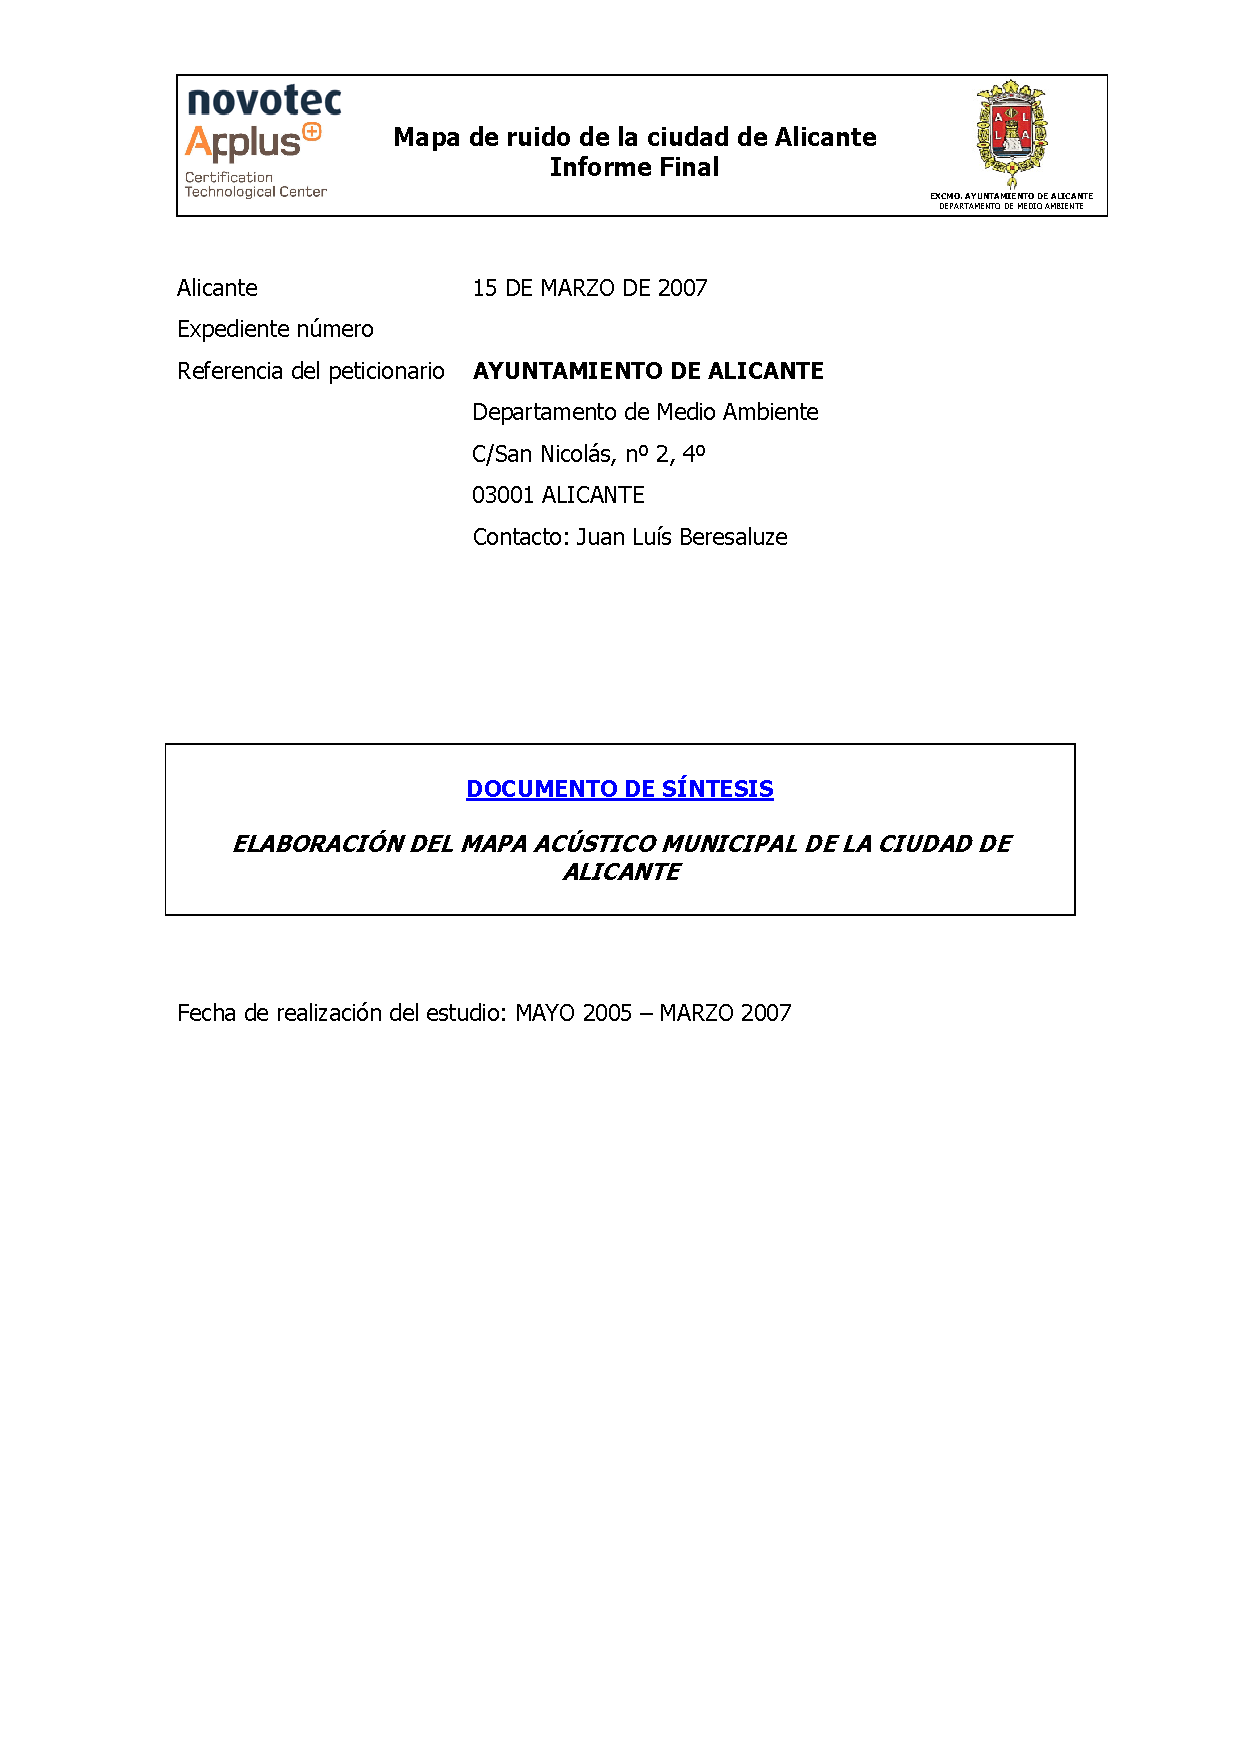
\includepdf[pages={1}]{archivos/ES_a_DF7_Agg_Alicante.pdf}

% Para incluir una página:
% [pages={0}] % Donde '0' es el número de la pagina del PDF que se quiere incluir

% Para incluir varias páginas consecutivas
% [pages={1-4}] % Con estos valores importa de la página 1 a la 4.

% Para incluir varias páginas salteadas
% [pages={1,4,7,10}] % Incluye las páginas 1,4,7 y 10

% Para incluir todo el documento PDF
% [pages=-]

% Si ademas de pages=... se incluye landscape, se importa en horizontal
% [pages{1},landscape]

\end{document}
